\documentclass{book}
\usepackage[a4paper,top=2.0cm,bottom=2.0cm,left=2.0cm,right=3.0cm]{geometry}

%\documentclass[pdftex,10pt,a4paper]{book}
%\usepackage[paperwidth=19cm,
%paperheight=26cm, outer=2cm, 
%top=1.5cm, bottom=1.5cm]{ geometry}

\usepackage[english,italian]{babel} %l'ultima lingua è quella che legge per i titoli
\usepackage[utf8]{inputenc}
\usepackage[T1]{fontenc,url}
\usepackage{titlesec}
\usepackage{easylist}
\usepackage{hanging}

\usepackage[pdftex,colorlinks]{hyperref}
\hypersetup{
	colorlinks=true,
	linkcolor=black,
	filecolor=magenta,
	urlcolor=cyan,
}
\usepackage{hypcap}
\usepackage{blindtext}
\usepackage{tipa}
\usepackage{epigraph}
\usepackage{enumerate}
\usepackage{longtable}
\usepackage{setspace}
\usepackage{verbatim}
\usepackage{graphicx}
\usepackage{amsmath}
\usepackage{pbox}
\usepackage{fancyhdr}
\usepackage{cancel}
\usepackage{tabularx}
\usepackage{booktabs}
\usepackage{multirow}
\usepackage{longtable}
\usepackage{tikz}
\usepackage{tikz-qtree}
\usepackage{subfig}
\usepackage{xcolor}
\usepackage{amssymb}
\usepackage{amsmath}
\usepackage{mathrsfs}
\usepackage{textcomp}
\usepackage{circuitikz}
\usepackage{pifont}
\usepackage{imakeidx}
\usepackage{verbatim}
\usepackage{dsfont}
\usepackage{listings}
\usepackage{color}
\usepackage{upgreek}
\usepackage{tasks}
\usepackage{exsheets}
\usepackage{pgfplots}
\usepackage{amsthm}
\usepackage{wasysym}


\usepackage{showframe}
\renewcommand\ShowFrameLinethickness{0.15pt}
%\renewcommand*\ShowFrameColor{\color{red}}

%\usepackage{showkeys} %serve per mostrare le etichette "tag" o target, va tolta per la versione definitiva;

\SetupExSheets[question]{type=exam}

\definecolor{mygreen}{rgb}{0,0.6,0}
\definecolor{mygray}{rgb}{0.5,0.5,0.5}
\definecolor{mymauve}{rgb}{0.58,0,0.82}

\lstset{ 
  backgroundcolor=\color{white},   % choose the background color; you must add \usepackage{color} or \usepackage{xcolor}; should come as last argument
  basicstyle=\footnotesize,        % the size of the fonts that are used for the code
  breakatwhitespace=false,         % sets if automatic breaks should only happen at whitespace
  breaklines=true,                 % sets automatic line breaking
  captionpos=b,                    % sets the caption-position to bottom
  commentstyle=\color{mygreen},    % comment style
  deletekeywords={...},            % if you want to delete keywords from the given language
  escapeinside={\%*}{*)},          % if you want to add LaTeX within your code
  extendedchars=true,              % lets you use non-ASCII characters; for 8-bits encodings only, does not work with UTF-8
  firstnumber=1000,                % start line enumeration with line 1000
  frame=single,	                   % adds a frame around the code
  keepspaces=true,                 % keeps spaces in text, useful for keeping indentation of code (possibly needs columns=flexible)
  keywordstyle=\color{blue},       % keyword style
  language=Octave,                 % the language of the code
  morekeywords={*,...},            % if you want to add more keywords to the set
  numbers=left,                    % where to put the line-numbers; possible values are (none, left, right)
  numbersep=5pt,                   % how far the line-numbers are from the code
  numberstyle=\tiny\color{mygray}, % the style that is used for the line-numbers
  rulecolor=\color{black},         % if not set, the frame-color may be changed on line-breaks within not-black text (e.g. comments (green here))
  showspaces=false,                % show spaces everywhere adding particular underscores; it overrides 'showstringspaces'
  showstringspaces=false,          % underline spaces within strings only
  showtabs=false,                  % show tabs within strings adding particular underscores
  stepnumber=2,                    % the step between two line-numbers. If it's 1, each line will be numbered
  stringstyle=\color{mymauve},     % string literal style
  tabsize=2,	                   % sets default tabsize to 2 spaces
  title=\lstname                   % show the filename of files included with \lstinputlisting; also try caption instead of title
}

% definizioni
\newtheorem{esercizio}{Esercizio}
\newtheorem{teorema}{Teorema}
\newtheorem{nota}{Nota}
\newtheorem{defi}{Definizione}
\newtheorem{esempio}{Esempio}
\newtheorem{svol}{Svolgimento}
\newtheorem{pro}{Proprietà}
\linespread{1.2} % l'interlinea

\frenchspacing

\newcommand{\abs}[1]{\lvert#1\rvert}

\usepackage{floatflt,epsfig}

\usepackage{multicol}
\newcommand\yellowbigsqcup[1][\displaystyle]{%
  \fboxrule0pt
  \ifx#1\textstyle\fboxsep-0.6pt\else\fboxsep-1.25pt\fi
  \mathrel{\fcolorbox{white}{yellow}{$#1\bigsqcup$}}}

\title{Appunti di Matematica}
\author{Nicola Ferru}
\date{}
\makeindex[columns=3, title=Alphabetical Index, intoc]

\begin{document}
%\maketitle
\begin{titlepage}
%	\tikz[remember picture,overlay] \node[opacity=0.50,inner sep=0pt, scale=0.8] at (current page.center){\includegraphics[width=\paperwidth,height=\paperheight]{./backround/backround.png}};
	\begin{center}
		
		% Upper part of the page
		
\includegraphics[scale=.45]{./title/logo_CA.jpg}
		\\
		\vspace{1cm}
		\textsc{\large Università degli Studi di Cagliari}
		\vspace{1.2cm}
		
		\textsc{\Large DIEE}
		\vspace{0.5cm}
		
		\textsc{\large Dipartimento di Ingegneria Elettrica, Elettronica e Informatica}
		\vspace{1.0cm}
		
		\textsc{\large Corso di Laurea {Triennale} in Ingegneria Elettrica}\hspace{0.8cm}
		
		% Title
		\vspace{0.8cm}
		
		\Huge \doublespacing \bfseries \begin{spacing}{1}{CHIMICA}\end{spacing}
		\hfill
		\normalsize \itshape \begin{spacing}{1}{}\end{spacing}
		\hfill
		\normalsize\itshape \begin{spacing}{1}{edited by}\end{spacing}
		\hfill
		\Large\itshape  \begin{spacing}{1}{NICOLA FERRU}\end{spacing}
		\vspace{0.5cm}
		%		% Author and supervisor
		%		\begin{flushleft} \large
			%			\emph{Relatore:} \\
			%			Ch.mo Prof. Nome \textsc{Cognome}
			%		\end{flushleft}
		%		\vfill
		%		\begin{flushright} \large
			%			\emph{Laureando:}\\
			%			Nome \textsc{Cognome}
			%			
			%			\textsc{Matricola N. 1234567}
			%		\end{flushright}
		
		\hfill
		\vfill
		\Large \bfseries \begin{spacing}{1}{Unofficial Version}\end{spacing}
		\vspace{0.5cm}
		% Bottom of the page
		%{\small 4 Ottobre 2018 -  \today{}}
		{\small 2021 -  2022}
	\end{center}
	\clearpage
	\thispagestyle{empty}
	\vspace*{\fill}%
	{\centering [This page is intentionally left blank]\par}%
	\vspace{\fill}
\end{titlepage}

\tableofcontents
%\listoftables
\listoffigures

\section{Premesse\dots}

In questo repository, inoltre,  sono disponibili le dimostrazioni grafiche realizzate
con \textit{Geogebra}; consiglio a tutte le persone che usufruiranno di questo lavoro, di dare un occhiata alle dimostrazioni grafiche e stare attenti,  in quanto nel tempo potranno  essere presenti delle modifiche, cosi da apportare miglioramenti al contenuto degli stessi appunti.  Solitamente il lavoro di revisione viene fatto tre/quattro volte alla settimana perché sono in piena fase di sviluppo.  Ricordo a tutti che essendo un progetto volontario ci potrebbero essere dei rallentamenti per cause di ordine superiore e quindi
potrebbero esserci meno modifiche del solito oppure essere presenti degli errori.  Chiedo pertanto  la cortesia a voi lettori di contattarmi per apportare eventuali correzioni .  Tengo a precisare che tutto il progetto è puramente open source, pertanto vengono resi disponibili i sorgenti dei file LaTex  insieme ai PDF compilati.

\begin{center}
	Cordiali saluti
\end{center}
\newpage

\section{Simboli}
\begin{multicols}{3}
	$\in$ Appartiene\\
	$\notin$ Non appartiene\\
	$\exists$ Esiste\\
	$\exists !$ Esiste unico\\
	$\subset$ Contenuto strettamente\\
	$\subseteq$ Contenuto\\
	$\supset$ Contenuto strettamente\\
	$\supseteq$ Contiene\\
	$\Rightarrow$ Implica\\
	$\Longleftrightarrow$ Se e solo se\\
	$\neq$ Diverso\\
	$\forall$ Per ogni\\
	$\ni :$ Tale che\\
	$\leq$ Minore o uguale\\
	$\geq$ Maggiore o uguale\\
	$\alpha$ alfa\\
	$\beta$ beta\\
	$\gamma$ gamma\\
	$\Gamma$ Gamma\\
	$\delta,\Delta$ delta\\
	$\epsilon$ epsilon\\
	$\sigma,\Sigma$ sigma\\
	$\rho$ rho
\end{multicols}

\chapter{Introduzione}
\label{chap:intro}
\section{Sommario}
Qui di seguito sono riportati i concetti fondamentali trattati all'interno del documento
\subsection{Informazione e segnali}
\label{sec:Informazioneesegnali}
L'informazione sussiste solo se il ricevente della trasmissione non conosce il
contenuto della suddetta.\\ Per esistere una trasmissione devono esserci:
\begin{enumerate}
  \item Comunicazione;
  \item Mezzo di trasmissione;
  \item Informazione.
\end{enumerate}

\subsection{Informazioni analogiche e digitali}
\label{sec:andiginfo}
Visto che è un argomento riccorrente all'interno del programma è giusto dare quanto
meno, una definizione anche se stringata, quindi:
\begin{defi}
  \label{def:andef}
  si dicono grandezze analogiche quelle che possono assumere tutti i valori
  intermedi all'interno di un dato intervallo; Si dicono grandezze digitali
  quelle che vengono espresse in modo numerico, senza possibilità di
  discriminare valori intermedi tra due cifre consecutive.
  Ulteriori approfondimenti presenti in (\ref{sec:sanalog})
  \footnote{\href{https://it.wikipedia.org/wiki/Analogico}{https://it.wikipedia.org/wiki/Analogico}}
\end{defi}
\begin{defi}
  \label{def:digdef}
  Con digitale o numerico, in informatica ed elettronica, ci si riferisce a tutto ciò che
  viene rappresentato con numeri o che opera manipolando numeri, contrapposto all'analogico. Ulteriori approfondimenti presenti in (\ref{sec:sdigital})
  \footnote{\href{https://it.wikipedia.org/wiki/Digitale_(informatica)}{https://it.wikipedia.org/wiki/Digitale\_(informatica)}}
\end{defi}
\begin{oss}
  \label{oss:strumMisura}
  Tipicamente quando si tratta di strumenti di misurazione entrambi i tipi di
  informazione entrano in gioco per poter funzionare. Ad esempio una sonda per
  un formo prende in ingresso in informazione analogica ``la temperature'' e poi
  la converte tramite l'apposito ADC a un informazione digitale per poterla
  campianare ed elaborare tarmite una centralina di gestione. 
\end{oss}
Oggi ormai utilizziamo il digitale perché effettivamente i calcolatori
elettronici gestiscono meglio una codifica rispetto a dei numeri reali. Per di
più costa meno produrre un dispositivo che gestisca segnali digitali rispetto
ad un dispositivo che gestisce mezzi analogici.
Ad esempio la differenza tra lo standard VHS e lo standard CD/DVD/Blue Ray, infatti,
il VHS era uno standard basato su un nastro magnetico, cosa che negli ultimi suoi anni
di vita si mescolò anche con il digitale ma uno dei limiti veri restava proprio il
supporto fisico, infatti, il nastro magnetico è molto fragile e incline ad avere
tantissimi problemi anche di prestazioni in utilizzi di archiviazione dati.
\subsection{Alcune osservazioni}
\begin{itemize}
\item Non tutte le informazioni costituiscono un vero e proprio contenuto
  inforamtivo
  \begin{enumerate}
  \item La notizia comunicata deve per noi essere eclatante;
  \item una persona noiosa non apporta informazione perché ripete
    continuamente gli stessi argomenti.
  \end{enumerate}
\item Problema di misurazione del contenuto informativo
  \begin{itemize}
  \item {\bf Claude E. Shannon} ({\tt 1916-2001}), fondatore della
    \textit{Teoria Matematica dell'Informazione}, è stato il primo
    ad introdurre la distinzione tra forma e significato nel
    processo comunicativo.
  \end{itemize}
\end{itemize}
\subsubsection{I risultati di Shannon}
\begin{itemize}
	\item Non è possibile definire la quantità di informazione associata ad un
		messaggio già ricevuto, ma piuttosto la quantità di informazione
		associata ad un papabile messaggio
		\begin{itemize}
			\item \textit{``information is that which reduces uncertainty''}
		\end{itemize}
	\item La quantità di informazione associata ad un massaggio è tanto più
		altra quanto più esso è inatteso
		\begin{itemize}
			\item il messaggio ``{\bf domani sorgerà il sole}'' ha un bassissimo
				contenuto informativo perché è assolutamente scontato e banale
			\item il messaggio ``{\bf Domani scoppierà la guerra}'' ha un alto
				contenuto informativo.
		\end{itemize}
\end{itemize}
\section{I segnali}
\begin{itemize}
	\item \textit{Grandezze fisiche variabili nel tempo a cui è associata
		un'informazione};
	\item \textit{L'informazione è associata ad una variazione ({\color{red}
		aleatorio} e non deterministica) della grandezza fisica};
	\item Aleatorio (dal latino ``alea'', gioco di dati) è sinonimo di non
		predicibile a priori (in contrapposizione con deterministico).
\end{itemize}
\subsection{Rappresentazione dell'informazione}
\label{sec:rappredellinfo}
\begin{itemize}
\item Associazione tra caratteristiche (di valore e temporali) dei segnali
  e le informazioni che essi rappresentano;
\item Le caratteristiche sono impresse dal dispositivo generatore del
  segnale;
\item Quali caratteristiche?
  \begin{itemize}
  \item valore, andamento temporale ed eventi del segnale (es.
    superare una soglia), etc.
  \end{itemize}
\end{itemize}
\subsection{Classificazione di segnali}
\label{sec:classsegn}
I segnali vengono classificati in base alla loro natura e alle loro caratteristiche.
Tipicamente per il campionamento avviene il seguente processo:
\begin{center}
  Grandezza fisica \textrightarrow{} trasduttore \textrightarrow{} segnale elettrico 
\end{center}
Quindi prendendo come base questa affermazione, possiamo dire che un segnale che sia
di natura elettrica, acustica o qualunque altra natura fisica, può essere campionato
da uno strumento che tramite il suo trasduttore converdirà in un istruzione
``tipicamente definita pacchetto di istruzioni o di informazioni'' che a sua volta
verrà convertito in un segnale elettrico che seguendo lo standard di comunicazione
del modello\footnote{una variazione della corrente elettrica o di tensione all'interno
  di un conduttore oppure in un punto di un circuito elettrico o elettronico.} di
rifimento potrà essere trasmesso o elaborato da un computer o da una centralina
dedicata a scopo di analisi oppure per inviarlo altrove. Ad esempio, se noi campioniamo
una chitarra elettrica sfruttando un pickup magnetico, il processo sarà il seguente:
\begin{center}
  Vibrazione della corda [\textit{pickup}] \textrightarrow{} scheda audio
  \textrightarrow{} segnale elettrico che il computer può leggere
\end{center}
Ed ecco come associare un caso di quotidiano all'argomento, infatti, la pratica qui
illustrata è un aspetto molto presente nella nostra vita, molti degli oggetti che
circondano la vita dell'individuo seguono questa logica.
\section{Spiegazione sui segnali}
\label{sec:spsegn}
\subsection{Segnali analogici}
\label{sec:sanalog}
\begin{itemize}
\item il valore dell'informazione rappresentata è una funzione continua
  della grandezza significativa;
\item rappresentazione attraverso un numero reale (\textit{con precisione
    teoricamente infinita})
\item generati da sensori o trasduttori che creano una corrispondenza tra
  la grandezza fisica che è oggetto di informazione (\textbf{esempio
    temperatura}) e il segnale (\textbf{esempio tensione elettrica})
\end{itemize}
\subsubsection{Esempi}
\begin{itemize}
	\item \textbf{Temperatura:} altezza in \texttt{mm} del mercurio nel
		termometro;
	\item \textbf{Acustico:} variazione di pressione ad un microfono;
	\item \textbf{Elettrico:} tensione ai capi di un conduttore.
\end{itemize}
\subsection{Segnali digitali}
\label{sec:sdigital}
\begin{itemize}
	\item rappresentazione come sequenza di numeri presi da un insieme di
		valori discreti, ovvero appartenenti a uno stesso insieme ben definito
		e circoscritto;
	\item rappresentazione ``{\bf a fasce}''
\end{itemize}
\begin{oss}
  L'attributo ``analogico'' o ``digitale'' non si riferisce a caratteristiche
  intrinseche del segnale ma a caratteristiche dell'informazione da esso rappresentato:
  {\color{red} I segnali digitali nascono come analogici}
\end{oss}
\subsection{Pregi e difetti}
\label{sec:pregiedifettideisegnali}

\subsubsection{Analogico}
\label{sec:analdifpreg}
\paragraph{Pregi}

\begin{tasks}(2)
	\task Sono più ``naturali'', le leggi della fisica classica operano
	tipicamente nel ``continuo'';
	\task Il rumore deforma ma non stravolge il segnale (errori proporzionali
	all'entità del disturbo ``{\bf in onde media la radio analogica la senti,
	anche se con un forte rumore bianco di fondo.}'')
\end{tasks}
\paragraph{Difetti}
\begin{tasks}(2)
	\task Dispositivi di elaborazione relativamente poco precisi, poco stabili
	nel tempo ``maggiormente predisposti ai guasti, alle intemperie e anche a
	potenziali variazioni atmosferiche'' e poco immuni alle perturbazioni;\\
	({\tt esempio}: il video registratore VHS ``M-matic'' o sony U-matic, sono
	apparecchi estremamente complessi, soprattutto gli ultimi per metà digitali
	con tante funzionalità e tasti programmabili per fasce orarie, perfetti per
	registrale le trasmissioni in modo autonomo.)
	\task Le elaborazioni su di essi sono poco flessibili e producono degrado.
\end{tasks}
\clearpage
\section{Il sistema numerico binario}
\label{sec:sistemanumbin}
\begin{defi}
  il sistema numeri Binario è un sistema di numerazione utilizzato per i calcolatori
  elettronici e sviluppato per soperire a lato prestazionale di calcolo per i
  suddetti\footnote{Un calcolatore elettronico riesce a processare più velocemente
    casi che possono avere poche possibilità, il binario per singola posizione può
    avere solo due possibilità 0 o 1}. Infatti, nel segnale digitale esite il seguente
  caso:
  \begin{itemize}
  \item 1 sta al Vero logico, in gergo ``TRUE'' oppure livello alto, in gergo ``HIGH''.
  \item 0 sta al Falso logico, in gero ``FALSE'' oppure livello basso, in gergo ``LOW''.
  \end{itemize}
  Il vantaggio di questo sistema è che con la logica positiva o negativa, risolve molti
  casi, tra cui il fatto che il singolo termine ``bit'' non sia segnato\footnote{Non è
    positivo o negativo, per avere il corrispettivo decimale con il segno si usa una
    codifica sacrificando un bit per attribuirgli la funzione di segno, se esso è pari a
    0 il numero, mentre, se il bit di segno è pari a 1 il numero è negativo.}, questo
  lo si vedrà nel dettaglio nei dettaglio in (\ref{<-->}) 
\end{defi}

\subsection{La rappresentazione}
\label{sec:rapbin}

La cosa comoda del sistema binario è il fattore di conversione, infatti, questa
codifica permette di rappresentare un qualunque numero decimale senza segno compreso
tra $0$ e $2^n-1$ tramite una sommatoria per posizione, come spressa nella seguente
formula:
\begin{equation}
  \label{eq:rappbin}
  (a_{n-1},\dots,a_1,a_0)_2\to \sum\limits^{n-1}_{i=0} a_i,b^i
\end{equation}
Dove $(a_{n-1})$ è la cifra più significativa e $a_0$ è quella meno significativa.
\begin{equation}
  \label{eq:esempiodiconversione}
  (10101110)_2\Leftrightarrow (174)_{10} \Leftrightarrow (AE)_{16}
\end{equation}

\subsection{Rappresentazione del modulo e del segno}
\label{sec:modesegnoinbin}
Il bit più significativo viene utilizzato per la rappresentazione del segno, mentre
il resto viene utilizzato per il modulo.
\begin{nota}
  questo sistema fa perdere un bit di rappresentazione quindi il valore rappresentato è
  pari al N-1, ad esempio su 8 bit che consentono di rappresentare fino al
  valore $(256)_{10}$ se andiamo ad applicare il bit segnato avremmo 7bit di
  rappresentaione per il modulo e 1bit per il segno cosa che porta la rappresentazione
  possibile al massimo a $(127)_{10}$ e $(-128)_{10}$
\end{nota}
Ma per essere più specifici meglio utilizzare una somma in forma tabellare per mostrare
l'esito dei segni in una somma tra due numeri $A$ e $B$:
\begin{equation}
  \label{eq:sommabin1}
  \begin{matrix}
    & \text{Segno di } B\\
    \text{Segno di } A &
                       \begin{array}{|ccc|}
                         &+&-\\
                         +& A+B & A-\abs{B}\\
                         - & B-\abs{A} & \abs{A}+\abs{B}
                       \end{array}
  \end{matrix}
\end{equation}

\subsection{Rappresentazione di complemento a 1}
\label{sec:rappcompa1}
Il bit più significativo rappresenta il segno, come nel caso di qui sopra
\begin{itemize}
\item stesso intervallo di valore rappresentabili con modulo e segno.
\end{itemize}
Un numero negativo si ottiene dal positivo cambiando tutti i bit:
\begin{itemize}
\item Il numero 6 in binario si scrivi 0110 prendeno un caso a 4 bit segnati ma
  se noi vediamo come si scrive il -6 il risultato è il seguente 1001 l'esatto inverso
  del numero positivo.
\end{itemize}
nelle operazione aritmetiche si utilizza l'eventuale riporto necessario a compensare
la mancanza di altri simboli al difuori dello 0 e del 1.
\begin{esempio}
  Prediamo una semplice somma come $22+3=25$, in questo caso per rappresentare
  l'operazione in colonna sono stati disposti 8 bit nonostante i numeri non sforino
  i 6.
  \begin{equation}
    \label{eq:compa1}
    \begin{array}{lccr}
      &&{\color{red}1100}&\\
       & 0001 & 0110 & (22)\\
      +& 0000 & 0011 & (3)\\\hline
       & 0001 & 1001 & (25)
    \end{array}
  \end{equation}
  I bit in rosso sono il riporto, infatti in questo caso è bastato solo un complemento a
  1 in cui il riporto non sfora dal numero di bit stimati, in gergo tecnico si tratta
  di un overflow, cosa che se avviene all'interno di un programma sul proprio computer
  può causare dei problemi, che siano di memoria perché satura la ram, potrebbe
  compromettere un altro processo se va a scrivere in un aria di memoria non adibito
  al suddetto processo oppure semplicemente se è un calcolo esso verrà tagliato e
  quindi barliamo di perdita di informazione.
\end{esempio}
\subsection{Rappresentazione di complemento a 2}
\label{sec:rappcompa2}
Il complemento a 2 è molto similare al complemento a 1 visto nel capitolo
(\ref{sec:rappcompa1}) con due sostaziali differenze -- La prima è un vantaggio,
infatti, in questo caso esiste un unica rappresentazione per lo zero, mentre,
la seconda è il fatto che si ignora l'overflow visto che i riporti molte volte
supereranno il valore rappresentabile.
\begin{esempio}
  Prendendo una semplice somma $31-5=26$, andiamo a fare il complemeto a due sfruttando
  in questo caso gli 8 bit pieni per il riporto, anche in questo caso le basi dei due
  addendi non superano i 6 bit ma per una questione di convenzione ``si usano basi
  multipli di 2, quindi il numero di bit devono essere 4, 8, 16, 32, 64, etc\dots''
  \begin{equation}
    \label{eq:compa2}
    \begin{array}{lccr}
      &{\color{red}1111}&{\color{red}1110}\\
      &0001&1111&(31)\\
      +&0000&1011&(-5)\\\hline
      &0001&1010&(26)
    \end{array}
  \end{equation}
  La differenza tra l'operazione (\ref{eq:compa1}) e la (\ref{eq:compa2}) sono poche
  ma significative, come si vede, i bit di riporto arrivano fino a sforare gli 8 bit
  nonostante ciò il risultato si ferma giustamente al quinto bit che im qiest caso
  è il più significativo e l'effetto del riporto sull'uno nella quarta posizione a
  partire da sinistra resta immutato proprio in virtù di quel principio.
\end{esempio} 
\subsection{Confronto}
\label{sec:controntotracomplementi}

\begin{table}[h!]
	\centering
	\begin{tabular}{|c|c|c|c|c|c|c|}
		\hline
		\multirow{2}{*}{Stringa}&\multicolumn{4}{c|}{rappresentazione}\\
		&senza segno&modulo e segno&complemento a 1&complemento a 2\\\hline
		000&0&0&0&0\\\hline
		001&1&1&1&1\\\hline
		010&2&2&2&2\\\hline
		011&3&3&3&3\\\hline
		100&4&0&-3&-4\\\hline
		101&5&-1&-2&-3\\\hline
		110&6&-2&-1&-2\\\hline
		111&7&-3&0&-1\\\hline
	\end{tabular}
	\caption {Confronto tra il modulo e segno, complemento 1 \& 2}
\end{table}

\section{Sistemi di comunicazione}
\label{sec:siscom}
Per poter rendere utile l'informazione è necessario per forza di cose che esistano degli
standard per poter comunicare, dei canali di comunicazione e dei sistemi dedicati alle
comunicazioni, ad esempio un libro consente di acquisire delle informazioni mediante
la scrittura che è codificata con dei caratteri in una determinata lingua oppure
un esempio ancora più immediato, prendiamo una comunicazione verbale tra due persone,
in quel caso il sistema di comunicazione è composto dai due individue, dall'aria che è
il canale di comunicazione e dalla lingua che è la codifica, se anche solo uno dei punti
non è soddisfatto la comunicazione non è efficace ``se i due individue parlano lingue
diverse non si va da nessuna parte'' non non avviene proprio ``in assenza d'aria non
si può parlare''
\subsection{Trasmissione e recezione}
\label{sec:trasmerec}
Il sistema di comunicazione per essere efficente prevede due elementi; la trasmissione
e la recezione che funzina nel guente modo:

\subsubsection{La trasmissione}
\label{sec:trasm}
Come visto in (\ref{sec:classsegn}) l'acquisizione di una informazione avviene
mediante un trasduttore che consente una conversione in un formato comprensibile
al calcolatore dopo che viene fatto questo processo di trasformazione tramite il
trasduttore sarà anche possibile diffonderlo tramite un canale di comunicazione.
\begin{center}
  Sorgente fisica \textrightarrow{} Trasduttore \textrightarrow{} TX \textrightarrow{}
  Al canale di comunicazione
\end{center}
Come chiaro dai passaggi, il TX ``dispositivo adito alla trasmissione'' è posto dopo
il trasduttore per motivi puremante essenziali, il messaggio per poter assere inviato
deve essere prima trasformato o per meglio dire tradotto in una codifica che sia chi
sta trasmettendo sia chi poi dovrà ricevere il suddetto messaggio devono conoscere,
altrimenti la comunicazione non riesce. Ovviamente il sengale nel canale di
comunicazione rispetterà criteri analogici e fisici per essere trasmesso, poi del
riportare l'istruzione alla forma leggibile ci penserà ricevitore.
\subsubsection{La recezione}
\label{sec:recezione}
Il processo di recezione è l'esatto opposto di quello di trasmissione, infatti,
presuppone che ci sia uno strumento in ascolto per catturare il segnale emesso,
infatti, il primo step nella catena di recezione è priprio il canale di comunicazione
\begin{center}
  Dal canale di communicazione \textrightarrow{} RX \textrightarrow{} Trasduttore
  \textrightarrow{} Utente finale
\end{center}
In questo caso il RX è il dispositivo in ascolto, poi ci sarà il trasduttore che
trasformera il segnale in un formato leggibile e poi l'utente finale che usufruira
dell'informazione acquisita.
\subsection{Classificazione di sistemi}
\label{sec:classidisistemi}
\begin{table}[ht]
  \centering
  \begin{tabular}{ll}
    \textbf{Punto-Punto} & \textbf{Multi-utente}\\\hline
    1 trasmettitore & 1 o più trasmettitore iniziali\\\hline
    1 o più ripetitori intermedi & 1 o più ripetitori\\\hline
    1 ricevitore & Il canale è una risorsa condivisa tra i diversi\\
                         & trasmettitori e/o ricevitori presenti nel sistema\\\hline
    Ad ogni tratto vengono associati uno o più & broadcast se coinvolge tutti gli utenti\\
    mezzi fisici di propagazione del segnale & come ricevitori.\\\hline
    Il canale è una risorsa dedicata al collegamento\\\hline
  \end{tabular}
  \caption{Classi di sistemi}
  \label{tab:classificazionedisistema}
\end{table}

\subsection{Rete di telecomunicazione}
\label{sec:retetele}

Quando si parla di reti di telecounicazioni si pensa sempre alla piattaforma tecnologica
su cui è basata, gli obbiettivi e le modalità di comunicazione.

\subsubsection{Obbiettivi}
\label{sec:obbiettivireti}
\begin{enumerate}
\item Effetuare comunicazione a distanza tra due o più utenti;
\item Trasferire informazione (servizio di telecomnicazioni) caratterizata diversi
  parametri (durata, qualità, etc.);
\item Gestire le sue parti componenti e i servizi supportati
\end{enumerate}
Ci sono diverse modalità (e dunque topologie) per realizzare tale trasferimento:
vantaggi/svantaggi.
\clearpage
\paragraph{Criteri di classificazione di reti}

La classificazione può essere basata sui seguenti criteri:
\begin{multicols}{2}
  \begin{enumerate}
  \item La gamma del servizi supportati;
  \item Grado di mobilità del terminale;
  \item l'Estensione fisica della rete;
  \item la posizione.
  \end{enumerate}
\end{multicols}

\subsection{Classificazione per servizi}
\label{sec:classperservizi}
Le reti vengono classificate anche per il criterio del servizio, infatti, esistono
reti dedicate, che svolgono solamente quel servizio e le reti integrata nei servizi
che consentono di svolgere più servizi con la stessa rete. Le differenze sono le
seguenti:
\begin{table}[ht]
  \centering
  \begin{tabular}{ll}
    Rete \textbf{Dedicata} ad un servizio & Reti \textbf{integrata nei servizi}\\\hline
    Fornitore di un singolo servizio & Fornitura di una vasta gamma di servizi\\\hline
    Possono essere utilizzate con alcune & Prestazioni complessive di qualità e di costo\\
    limitazioni anche per un insieme & decisamente migliori rispetto a quella ottenibile\\
    ristretto di altri servizi. & con le reti dedicate.\\\hline

    L'esempio: la rete telefonica fissa & L'esempio: Internet e le reti mobile della\\
    generazioni di reti mobili ({\it GSM}) & generazione 2G in poi.\\\hline
  \end{tabular}
  \caption{Classificazione per servizi}
  \label{tab:classperserv}
\end{table}
\begin{oss}
  Al giorno d'oggi è più diffusa la seconda categoria di rete perché costa meno e può
  svolgere più di un servizio e con il fatto che restano solo pochi sistemi anche la
  manutenzione costa meno e si possono investire i fondi per rendere tutto più stabile e
  tollerante ai guasti.
\end{oss}
\subsection{Classificazione per mobilità}
\label{sec:classificazionemobile}
\begin{table}[ht]
  \centering
  \begin{tabular}{ll}
    \texttt{Rete fissa} & \texttt{Rete mobile}\\\hline
    Gli utenti accedono alla rete da postazioni fisse, & gli utenti possono muoversi senza limitazioni\\
    oppure si muovono in un interno relativamente.  & al loro spostamenti (anche tramite veicoli) \\
    ristretto &\\\hline
    Il punto di accesso fisso, terminale può essere mobile & Gli utenti possono cambiare\\
                        & ``punto di accesso'' alla rete che gestisce ciò\\
                        &  rendendoli sempre raggiungibili (handever)\\\hline
    ad esempio terminali Wi-Fi che accedono ad Internet & ad esempio i cellulari\\\hline
  \end{tabular}
  \caption{Classificazione per mobilità}
  \label{tab:classipermobile}
\end{table}
\begin{nota}
  Le reti mobili hanno il vantaggio della portabilità del servizio ma hanno alcuni
  limiti, tra cui la copertura del proprio ISP (\underline{Internet Service Provider})
  e le prestazioni sono inferiori rispetto a quello cablato.
\end{nota}

\subsection{Classificazione per estensione}
\label{sec:classest}
Le reti di telecomunicazioni si suddividono anche per portata massima, questa
nomenclatura viene utilizzata per le reti internet e VoIP, partendo dalla più
piccola per portata la PAN alla più estesa la WAN. 
\begin{table}[ht]
  \centering
  \begin{tabular}{llll}
    PAN& LAN& MAN & WAN\\\hline
    Area personale & Area locale & Area relativamente estesa & Area molto estesa\\
    (circa 1m) & (max pochi km) & (Città, decina di km) & (nazione, centinaia di km)\\
    \hline
    Bluetooth & Ethernet, Wi-Fi & WiMAX & Internet, rete telefonica\\\hline
  \end{tabular}
  \caption{Classificazione per estensione}
  \label{tab:classest}
\end{table}

\subsection{Interconnessione di reti}
\label{sec:interdireti}
Uno dei fondamenti delle telecomunicazione è proprio l'interconnessione cioè la
possibilità di connettere più reti a sieme, infatti, esiste la possibilità di unire
più reti {\tt PAN} in una rete {\tt LAN}.
\begin{center}
  (PAN $\longleftrightarrow$ PAN $\longleftrightarrow$ PAN) LAN
\end{center}
Con questo sistema si ottengono reti di tipo omogeneo e si aggiungono opportuni
meccanismi e protocolli comini operanti sempre le varie reti componenti.

\subsection{Classificazione per posizione}
\label{sec:classperposiz}

Le reti di trasmissione interconnette tra di loro le reti di accesso permettendo le
comumicazioni tra terminali di utenti remoti collegati a differenti reti di accesso.
In riferimento alla rete più grossa di cui fa parte, viene anche chiamata
``Core Network''.
\begin{center}
  \Tree[.Rete\ di\ trasmissione rete\ di\ accesso rete\ di\ accesso rete\ di\ accesso ] 
\end{center}
Nel caso delle reti di accesso interconnette tra di loro i terminali presenti in un'area
limitata e questo con una rete di trasmissione.

\subsection{Soggetti implicati}
\label{sec:soggimp}

\begin{table}[ht]
  \centering
  \begin{tabular}{lll}
    \textbf{Gestore di rete}&\textbf{Fornitore del servizio}&\textbf{Cliente del servizio}\\\hline
    Network operator: attiva e mantiente & Service Provider: rende fruibile & Soggetto della \\
    operativa la piattaforma di rete per & il servizio al cliente secondo & comunicazione (sorgente e/o\\
    assicurare la fruizione dei servizio & modalità (e.g. costo, durata) & destinatario)
  \end{tabular}
  \caption{Soggetti implicati nella gestione del servizio di rete}
  \label{tab:sggimp}
\end{table}

\section{Rami e nodi}
\label{sec:ramienodi}
\begin{defi}
  La rete è un insieme di nodi e di rami quindi nel tempo
  sono nate diverse dopologie per sopperire alle esigenze. Al momento le topologie più
  diffuse sono:
  \begin{itemize}
  \item A maglia;
  \item A Stella o Grafo;
  \item Ad Nello.
  \end{itemize}
  Ne esistono anche delle altre ma non sono altrettanto diffuse. Alcune topologie
  non sono più utilizzate in quanto frutto dei primi esperimenti a riguardo ma non
  efficenti, altre non si sono diffuse per un puro andamento di mercato.
  Tra l'altro le topologie prima citate in un caso reale vengono mescelete per poter
  ottenere una maggiore tolleranza ai guasti. 
\end{defi}
\begin{figure}[ht]
  \centering
  \resizebox{10cm}{!}{\def\a{.4}
\def\b{.3}
\def\cr{.53}

\begin{tikzpicture}
% bus topograpy
\draw (2,-1) circle (\a cm);
\draw (2,-1) -- (2,0);
\draw (4,-1) circle (\a cm);
\draw (4,-1) -- (4,0);
\draw (1,1) circle (\a cm);
\draw (1,1) -- (1,0);
\draw (3,1) circle (\a cm);
\draw (3,1) -- (3,0);
\draw (5,1) circle (\a cm);
\draw (5,1) -- (5,0);
\draw (0,0) -- (6,0);

% star topograpy
\draw (10,0) -- (8.5,-1);
\draw (8.5,-1) circle(\b cm);

\draw (10,0) -- (11.5,-1);
\draw (11.5,-1) circle(\b cm);

% centro
\draw (10,0) circle(\cr cm);

\draw (10,0) -- (10,-1.7);
\draw (10,-1.7) circle(\b cm);

\draw (10,0) -- (9,1);
\draw (9,1) circle(\b cm);

\draw (10,0) -- (11,1);
\draw (11,1) circle(\b cm);

% Rete ad anallo

\draw (13.5,-1) circle(\b cm);
\draw (13.5,-1) -- (14.5,-1.7);
\draw (13.5,-1) -- (14,0.4);

\draw (15.5,-1) circle(\b cm);
\draw (14.5,-1.7) -- (15.5,-1);

\draw (14.5,-1.7) circle(\b cm);
\draw (15.5,-1) -- (15,0.4); 

\draw (14,0.4) circle(\b cm);

\draw (15,0.4) circle(\b cm);
\draw (14,0.4) --  (15,0.4);

% modello a maglia
\draw (17,-1) circle(\b cm);
\draw (19,-1) circle(\b cm);
\draw (17,-1) -- (19,-1);

\draw (17,-1) -- (18,-1.7);
\draw (18,-1.7) circle(\b cm);
\draw (18,-1.7) -- (19,-1);

\draw (18,-1.7) -- (17.4,0.4); 
\draw (17.4,0.4) circle(\b cm);
\draw (17,-1) -- (17.4,0.4);
\draw (17.4,0.4) -- (19,-1);

\draw (18.7,0.4) circle(\b cm);
\draw (18,-1.7) -- (18.7,0.4);
\draw (17,-1) -- (18.7,0.4);
\draw (17.4,0.4) -- (18.7,0.4);
\draw (19,-1) -- (18.7,0.4);
\end{tikzpicture}}
  \caption{Topologie a bus, a stella, ad anello e a maglie}
  \label{fig:topologiepiùutilizzate}
\end{figure}
\begin{oss}
  La topologia a bus era la prima topologia prevista per lo standard TCP/IP,
  infatti, funzionava tramite cavo coassiale cablato direttamente da una scheda
  di rete all'altra, questo sistema non sopravvisse a lungo per il semplice
  motivo che era poco efficente ma soprattutto il coassiale è un cavo semirigido
  e facilmente incline alla rottura, per non parlare dei connettori che hanno
  una tenuto non solida come gli attuali RJ45 e RJ14 per le linee telefoniche,
  come molti standard di questo tipo vengono dritti dal Bell Labs di AT\&T.
\end{oss}

\subsubsection{I significato}
\label{sec:significato}
\begin{defi}
  Il nodo è il mezzo di scambio tra due o più rami, o terminazione degli stessi,
  in questa categori fanno parte sia le terminazioni fisiche di rete che
  gli apparati di comunicazione.
\end{defi}
\begin{defi}
  Il ramo per definizione è il percorso diretto che l'informazione segue per essere
  trasferita tra due nodi, in questa categoria rientrano sia il mezzo trasmissivo che
  la giunzioni fisica/lagica tra due apparati di rete. 
\end{defi}

\subsubsection{Nodi intermedi e terminali}
\label{sec:nodiintermedi}
Il nodo intermedio (\texttt{nodo di commutazione o ralay})
\begin{itemize}
\item Il nodo di scambio, modulazione/demultiplazione;
\item A seconda dei casi viene chiamato Gateway, router, switch, digital cross
  connector, hub, repeater, etc.
\item Concetto simile a quello di parcheggio scambiatore.
\end{itemize}
Nodi terminali ({\it end system})
\begin{itemize}
\item I sorgente/destinazione della comunicazione;
\item Il mezzo attraverso cui un utente usufruisce di uno o più servizi di
  telecomunicazione;
\item Ia variazione di forma: TV, telefono fisso/mobile, PC, elettrodomestici
\end{itemize}
A seconda del livello di astrazione, un nodo può assumere una funzione o l'altra.

\subsection{Definizione di grafo}
\begin{defi}
  I grafi sono struttura matematiche discrete che rivestono interesse sia per la
  matematica che per un'ampia gamma di campi applicativi. In ambito matematico il loro
  studio, la teoria dei grafi, costituisce un'importante parte della combinatoria; i
  grafi inoltre sono utilizzati in aree come topologia, teoria degli automi, funzioni
  speciali, geometria dei poliedri, algebre di Lie. I grafi si incontrano in vari
  capitoli dell'informatica (ad esempio per schematizzare programmi, circuiti, reti di
  computer, mappe di siti). Essi inoltre sono alla base di modelli di sistemi e
  processi studiati nell'ingegneria, nella chimica, nella biologia molecolare, nella
  ricerca operativa, nella organizzazione aziendale, nella geografia (sistemi fluviali,
  reti stradali, trasporti), nella linguistica strutturale, nella storia
  ({\bf alberi genealogici, filologia dei testi})\footnote{\href{https://it.wikipedia.org/wiki/Grafo}{https://it.wikipedia.org/wiki/Grafo}}. 
\end{defi}
\label{sec:grafo}
\begin{figure}[ht]
  \centering
  \def\b{.3}
\def\cr{.53}
\begin{tikzpicture} 
%\draw (1.5,1.5) circle [radius=\cr];
\node at (1.5,4.5) {$N= ?$ $R=?$};
% centro a maglia
\draw (1.5,1) circle [radius=\b];
\draw (1,1.9) circle [radius=\b];
\draw (2,1.9) circle [radius=\b];
\draw (2,1.9) -- (1,1.9) -- (1.5,1) -- (2,1.9);
% end centro 

\draw (1.5,1) -- (0,0);
\draw (0,0) circle [radius=\b];

\draw (1.5,1) -- (1.5,0);
\draw (1.5,0) circle [radius=\b];

\draw (3,0) -- (1.5,1);
\draw (3,0) circle [radius=\b];

\draw (1,1.9) -- (0,3);
\draw (0,3) circle [radius=\b];

\draw (2,1.9) -- (3,3);
\draw (3,3) circle [radius=\b];

\draw (2,1.9) -- (2.5,3.7);
\draw (2.5,3.7) circle [radius=\b];
\end{tikzpicture}
  \caption{esempio di grafo}
  \label{fig:grafolesempio}
\end{figure}
\begin{itemize}
\item Per definire il Grafo si utilizza la formula:
  \begin{equation}
    \label{eq:grafodef}
    G=(V,A)
  \end{equation}
\item Insieme dei nodi (vertici)
  \begin{equation}
    \label{eq:insiemedeinodi}
    V\text{ con } N=\abs{V}
  \end{equation}
\item Insieme dei rami (archi)
  \begin{equation}
    \label{eq:insiemedeirami}
    A\text{ con } R=\abs{A}
  \end{equation}
\item Grafo orientato: si fa distinzione sul verso di percorrenza dei rami
\end{itemize}
\subsection{Topologie}
\label{sec:top}
Come descritto nel paragrafo esistono differenti topologie, nati per esigenze diverse e
anche in contesti diversi, con peculiarità relative alla costituzione fisica e logica
delle suddette e anche con formule matematiche adite a calcolare eventuali nodi massimi,
la portata della banda passante, etc.  

\subsection{Topologia Elementari}
\label{sec:topologieelementari}
Topologie lineari semplici
\begin{itemize}
\item Ciascun nodo è collegato a due nodi adiacenti con un solo ramo
\end{itemize}
Topologie lineari complesse (\texttt{a struttura gerarchica})
\begin{itemize}
\item Per ogni coppia di nodi esiste un solo percorso di collegamento
\item Ogni nodo è collegato con uno o più rami ai nodi di gerarchia inferiore
\end{itemize}
Topologie magliate
\begin{itemize}
\item Ogni nodo è connesso direttamente agli altri nodi, usando per ciascun
  collegamento un ramo dedicato
\end{itemize}
Topologie a bas
\begin{itemize}
\item Tutti i nodi condividono lo stesso unico collegamento
\end{itemize}

\subsubsection{Topologia a maglia completa}
\label{sec:topologiaamagliacompleta}
In questa topologia ogni nodo è collegato a tutti gli altri presenti, per questo motivo
ha un alta tolleranza ai guasti ma il grosso difetto è l'elevato numero di nodi e quindi
anche i conosti di mantenimento e di realizzazione.
\begin{figure}[ht]
  \centering
  \def\a{.4}
\def\b{.3}
\def\cr{.53}

\begin{tikzpicture} 
\draw (0,0) circle [radius=\a];
\draw (0,0) -- (2,0) -- (2.5,2) -- (1,3) -- (-0.5,2) -- (0,0) -- (1,3) -- (2,0) -- (-0.5,2) -- (2.5,2) -- (0,0);
\draw (2,0) circle [radius=\a];
\draw (2.5,2) circle [radius=\a];
\draw (-0.5,2) circle [radius=\a];
\draw (1,3) circle [radius=\a];
\end{tikzpicture}
  \caption{Esempio di topologia a maglia}
  \label{fig:topologiaamagliacompleta}
\end{figure}
\begin{oss}
  Per le sue caratteristiche questa topologia è utilizzata dagli ISP per i collegamenti
  stradali, infatti, per evitare che un'intera zona resti senza servizio solo perché
  un cavo si è rotto il metodo migliore risulta proprio il creare più di una strada
  per portare l'informazione, infatti, come precedentemente spiegato nei capitoli
  precedenti la topoligia davvero utilizzata in molti casi è ibrida.
\end{oss}
\begin{equation}
  \label{eq:magliacompleta}
  R=\sum\limits_{i=1}^N (N-i)=\sum\limits_{i=1}^N N - \sum\limits_{i=1}^N i = N^2-
  \frac{N(N+1)}{2} = \frac{N(N-1)}{2}
\end{equation}
\clearpage
\subsubsection{Topologia a stella}
\label{sec:topastellaegrafo}
La topologia a stella è una versione semplicifata di una topologia ad albero,
infatti, è una topologia a albero composto da un solo livello oltre alla radice.
Come tutte le topoligie ad albero soffre di un problema devastante, una bassissima
tolleranza ai guasti, se il centro del della rete si guasta o smette di funzionare
la rete non è più operativa, creando un disservizio ma questo modello ha anche pregi,
infatti, ha dei costi decisamente inferiori per l'allestimento e la manutenzione,
è facile da instradare e i nodi sono pochi.
\begin{figure}[ht]
  \centering
  \def\b{.3}
\def\cr{.53}
\begin{tikzpicture} 
\draw (1.5,1.5) circle [radius=\cr];
\draw (1.5,1.5) -- (0,0);
\draw (0,0) circle [radius=\b];
\draw (3,0) -- (1.5,1.5);
\draw (3,0) circle [radius=\b];
\draw (1.5,1.5) -- (0,3);
\draw (0,3) circle [radius=\b];
\draw (1.5,1.5) -- (3,3);
\draw (3,3) circle [radius=\b];

\draw (1.5,1.5) -- (1.5,3.7);
\draw (1.5,3.7) circle [radius=\b];
\end{tikzpicture}
  \caption{Esempio di topologia a stella}
  \label{fig:stellaesempio}
\end{figure}

\begin{oss}
  Questa topologia di rete è forse uno dei più diffusi, infatti, le reti domestiche sia
  ethernet sia Wi-fi funzionano proprio con un centro stella, il modem/router domestico
  svolge tante funzioni tra cui anche quello di switch e access point.
\end{oss}
In questo caso per calcolare $R$ basta calcolare il numero totale dei nodi-1, come
esposto dalla seguente formula
\begin{equation}
  \label{eq:stella}
  R=N-1
\end{equation}

\subsubsection{Topologia a maglia non completa}
\label{sec:topologiaamaglianoncompleta}
Questo risulta già un caso più generale e risulta un compromesso
tra una rete ad albero e una a maglia completa, i pregi sono una maggior
tolleranza ai guasti rispetto al modello ad albero, un numero a piacere di
rami. I difetti sono legati proprio alla topologia che risulta non regolare.
\begin{figure}[ht]
  \centering
  \def\a{.4}
\def\b{.3}
\def\cr{.53}

\begin{tikzpicture} 
\draw (0,0) circle [radius=\a];
\draw (0,0) -- (2,0) -- (2.5,2) -- (1,3) -- (-0.5,2) -- (2.5,2) -- (0,0);
\draw (2,0) circle [radius=\a];
\draw (2.5,2) circle [radius=\a];
\draw (-0.5,2) circle [radius=\a];
\draw (1,3) circle [radius=\a];
\draw (-2,1) circle [radius=\a];
\draw (-2,1) -- (-0.5,2);
\end{tikzpicture}
  \caption{Esempio di topologia a maglia non completa}
  \label{fig:topologiaamagliacompletanoncomp}
\end{figure}
\begin{oss}
  Questo è il modello più utilizzato dagli ISP perché risulta semplice sia in fase
  di manutenzione e anche il più vesatile avendo la possibilità di scegliere il numero
  di rami, quindi si può optare per mettere più nodi in percorsi in cui la banda
  passante è maggiore e meno dove non è necessario una tale tolleranza.
\end{oss}
In questo caso il valore $R$ risulta compreso tra la condizione dei sistemi ad albero e
quelli a maglia
\begin{equation}
  \label{eq:maglianoncompleta}
  N-1 < R < \frac{N(N-1)}{2}
\end{equation}
\clearpage
\subsubsection{Topologia ad anello}
\label{sec:topadan}
La rete ad anello non è molto diffusa, infatti, tipicamente viene utilizzata per
le reti locali e metropolitane, essa può essere unidirezionele ({\it quindi il giro che
  fa l'informazione è sempre lo stesso sia se il nodo è in prossimita o se più
  distante}) che bidirezionale e quindi prende il percorso più efficiente per instradare
l'informazione.
\begin{figure}[ht]
  \centering
  \def\a{.3}
\def\cr{.53}

\begin{tikzpicture}
\draw (0,0) circle [radius=\a];
\draw (0,0) -- (2,0) -- (2.5,2) -- (1,3) -- (-0.5,2) -- (0,0);
\draw (2,0) circle [radius=\a];
\draw (2.5,2) circle [radius=\a];
\draw (-0.5,2) circle [radius=\a];
\draw (1,3) circle [radius=\a];
\end{tikzpicture}
  \caption{Esempio di topologia ad anello}
  \label{fig:topologiaadanello}
\end{figure}
Questa topologia non è particolarmente tollerante ai quasti e basta la rottura di un
ramo per causare non poche rogne, soprattutto se il sistema è unidirezionale. In questo caso
la formula che tutela $R$ dipende esclusivamente dal numero di nodi.
\begin{equation}
  \label{eq:adanallo}
  R=N
\end{equation}

\subsection{Topologia a bus: unicast vs broadcast}
\label{sec:unicvsbroadcast}
\begin{figure}[ht]
  \centering
  \def\a{.3}

\begin{tikzpicture}
% unicast bus
\draw (0,0) circle [radius=\a];
\draw(1.5,0) circle [radius=\a];
\draw(3,0) circle [radius=\a];
\draw(4.5,0) circle [radius=\a];
\draw (0,0) -- (4.5,0);
\node at (2.2,-0.6) {Bus unicast $R=N-1$};

% brodcast bus
\draw (6,0) circle [radius=\a];
\draw (7.5,0) circle [radius=\a];
\draw (9,0) circle [radius=\a];
\draw (10.5,0) circle [radius=\a];
\draw (6,0) -- (6,1) -- (10.5,1) -- (10.5,0);
\draw (7.5,0) -- (7.5,1);
\draw (9,0) -- (9,1); 
\node at (8.2,-0.6) {Bus broadcast $R=1$};
\end{tikzpicture}
  \caption{Topologia a bus unicast e broadcast}
  \label{fig:topologiaadanello}
\end{figure}

\subsubsection{Unicast}
\label{sec:unicast}

\begin{itemize}
\item Connessione a bus attivo punto-punto;
\item I nodo connessi in modo ``lineare'';
\item Ogni nodo partecipa alla comunicazione tra le altre coppie di nodi;
\item Usata soprattutto in reti con cavo
\end{itemize}

\subsubsection{Broadcast}
\label{sec:broadcast}
\begin{itemize}
\item Il collegamento pra i nodi avviene tramite un unico mezzo di diffusivo (fisico o virtuale) tipo broadcast
\item Bus pasivo
\item La comununicazione avviene contemporaneamente da una a tutti
\item Usata pricipalmente in LAN e MAN (con e senza fili)
\end{itemize}

\subsection{Topologia generale di una rete}
\label{sec:topgenret}

In generale la topologia di una rete di telecomunicazione può essere una combinazione delle topologie precedenti
({\it tipologia mista})
\begin{itemize}
\item In alcuni casi una rete può essere anche rappresentata con una nuvola che interconnette i vari
  nodi terminali
\end{itemize}

\subsection{Sezione d'accesso}
\label{sec:sezioned'accesso}
La sezione d'accesso ha il ruolo di consentire l'accesso alla rete ai suoi utenti, viene realizzata attraverso
differenti mezzi e tecnologie
\begin{itemize}
\item Cablate (\textit{rame, fibra}) o senza fili
\item punto-punto o \textit{broadcast}
\end{itemize}
È la sede di risorse in alcuni casi dedicate ai singoli utenti/terminali -- Conprende l'interfaccia utente-rete.
\begin{itemize}
\item Tecnologie e processi utilizzati nel segmento terminale di un sistema di collegamento;
\item Ciò che permette il collegamento dell'utente con la rete;
\item Tratta di cavo che connette le centrali telefoniche agli utenti finali
\item \texttt{Essential farility:} elevati costi tecnologici
\item liberalizzazione e nuovi concerrenti
\end{itemize}

\subsection{Sezione interna}
\label{sec:sezint}
\begin{figure}[ht]
  \centering
  \def\a{.3}
\newcommand{\boundellipse}[3]% center, xdim, ydim
{(#1) ellipse (#2 and #3)
}


\begin{tikzpicture} 
	\draw (-2,2) -- (-2.5,0) -- (1,-1) -- (4,0.2) -- (4,2) -- (-2,2); 
	\draw (-2,2) -- (0,.5) -- (4,2);
	\draw (-2.5,0) -- (0,0.5) -- (4,0.2);
	\draw (-2.5,0) -- (-7,0);
	\draw (-2,2) -- (-1,3.97);
	\draw (1,-1) -- (0,-4);
	\draw (6,-2) -- (4,0.2) -- (7,0);
	\draw (4,2) -- (4.6,3);
	\node at (-1,4.5) {A};

	\draw[dashed] \boundellipse{0,0}{-7}{4};
	\draw[fill] (0,-4) circle [radius=\a];
	\draw[fill] (-1,3.97) circle [radius=\a];
	\draw[fill] (-7,0) circle [radius=\a];
	\draw[fill] (7,0) circle [radius=\a];
	\draw[fill] (4.6,3) circle [radius=\a];
	\draw[fill] (6,-2) circle [radius=\a];


	% centro a maglia
	\draw[color=blue,fill] (-2,2) circle [radius=\a];
	\draw[color=blue,fill] (-2.5,0) circle [radius=\a];
	\draw[color=blue,fill] (1,-1) circle [radius=\a];
	\draw[color=blue,fill] (0,0.5) circle [radius=\a];
	\draw[color=blue,fill] (4,0.2) circle [radius=\a];
	\draw[color=blue,fill] (4,2) circle [radius=\a];
	\node[color=white] at (1,-1) {T};

	\node at (-1,-5.3) {A: Nodi di accesso};
	\node at (-1,-6) {T: Nodi di transito};
\end{tikzpicture}
  \caption{Sezione interna}
  \label{fig:sezint}
\end{figure}

\begin{itemize}
\item Ha il ruolo di trasferire l'informazione tra nodi di accesso, se necessario, anche nodi di transito;
\item È sede di risorse condivise\footnote{di trasferimento e di elaborazione} con elevate prestazioni, in
  termini di velocità\footnote{trasmissiova ed elaborativa} e affidabile.
\end{itemize}
\subsection{Principali organismi}
\label{sec:princorg}

\begin{description}
\item[International Telecommunication Union (ITU):] Agenzia delle Nazioni Unite con il compito di armonizzare
  tutte le iniziative mondiali e regionali nel settore delle telecomunicazioni. Produce \texttt{raccomandazioni}
  con carattere volontario, ma di fatto linee guida fondamentali.
\item[International Standard Organization (ISO):] Ente delle Nazioni Unite creato con l'obiettivo di promuovere lo
  sviluppo della normativa internazionale per facilitare il commercio di beni e servizi nel mondo.
\item[Institute of Electrical and Electronics Engineers (IEEE):] Associazionee internazionale di scienziati
  professionisti con l'obbiettivo della promozione delle scienze tecnologiche, particolarmente attivo nella
  standardizzazione delle tecnologie per LAN e MAN.
\item[Internet Engineering Task Force (IETF):] È il gruppo preposto alla definizione degli standard nel mondo
  Internet. Chiunque può partecipare sottomettendo degli \textit{Internel-draft}. Vengono prodotte le cosiddetto
  \textit{Request For Comments} (RFC).
\item[Third Generation Parnership Project (3GPP):] 3GPP riunisce differenti organizzazioni e associazioni con
  l'obiettivo di produrre specifiche tecniche per la reti mobili di terza generazione.
\item[European Telecommunication Standards Institute (ETSI):] La preparazione degli standard è effettano
  da trattano argomenti specifici e che riferiscono ad una assemblea tecnica.
\end{description}
\section{Unità informative (UI)}
\label{sec:unitinfo}

Il mezzo attraverso il quale viene trasferita l'informazione, le UI possono essere:
\begin{itemize}
\item i singoli bit o byte (\textbf{1B=8b});
\item i blocchi/sequenze di bit o byte (di dimensione fissa o variabile);
\end{itemize}
\begin{nota}
  L'unità informativa può avere anche nomi alternativi: unità dati, pacchetti, messaggi, segmenti, trame, etc.
\end{nota}

\subsection{Tipi di informazione/traffico}
\label{sec:tipidiinformazione}
\begin{figure}[ht]
  \centering
  \resizebox{5in}{!}{\usetikzlibrary {arrows.meta} 

\begin{tikzpicture}
\node at (-2,1) {Informazione};
\draw (0,0) -- (4,0) -- (4,2)  -- (0,2)-- cycle;
\node at (2,1) {Utente};
\draw (4.5,0) -- (9.5,0) -- (9.5,2)  -- (4.5,2)-- cycle;
\node at (7,1) {segnalazione/controllo};
\draw (10,0) -- (14,0) -- (14,2)  -- (10,2)-- cycle;
\node at (12,1) {Gestione};

\node at (-2,-2) {Sotto-rete};
\draw (0,-3) -- (4,-3) -- (4,-1)  -- (0,-1)-- cycle;
\node at (2,-2) {Dati};
 \draw[-{Stealth[length=5mm]}]        (2,0)   -- (2,-1);
\draw (4.5,-3) -- (9.5,-3) -- (9.5,-1)  -- (4.5,-1)-- cycle;
\node at (7,-2) {segnalazione};
 \draw[-{Stealth[length=5mm]}]        (7,0)   -- (7,-1);

\draw (10,-3) -- (14,-3) -- (14,-1)  -- (10,-1)-- cycle;
\node at (12,-2) {Gestione};
 \draw[-{Stealth[length=5mm]}]        (12,0)   -- (12,-1);


\end{tikzpicture}}
  \caption{Tipi di informazione/traffico}
  \label{fig:traffic}
\end{figure}
\begin{oss}
  I diversi tipi di informazione possono in alternativa condividere la medesima infrastruttura di
  rete.
\end{oss}

\subsubsection{Informazione di utente}
\label{sec:infoutente}

\begin{itemize}
\item Obiettivo della comunicazione;
\item Differenti media (\textit{voce, dati, video});
\item Può essere inviata insieme a dell'extra-informazione aggiunta per scopi di controllo del trasferimento
  (\texttt{overhead});
\begin{esempio}
  Indirizzi, campi di controllo di errore, etc.
\end{esempio}
\item Coinvolge le funzionalità di trasporto della rete.
\end{itemize}

\subsection{Informazione di controllo}
\label{sec:infocont}
l'Informazione di controllo è di supporto affinché possa avvenire la comunicazione, permette di
\begin{itemize}
\item Inizializzare una comunicazione;
\item negoziarne le caratteristiche;
\item controllare il trasferimento dei dati di utente
\end{itemize}
Coinvolge le funzionalità di controllo.

\subsection{Informazione di gestione}
\label{sec:infodigest}

L'informazione di gestione in genere scambiata tra nodi di rete, ha lo scopo di consentire operazioni di
gestione delle risorse/apparati di rete -- \textbf{Operation Administration Management} (OAM)
\begin{itemize}
\item informazione per operazioni di esercizio;
\item informazioni per operazioni di amministrazione;
\item informazione per operazioni di manutenzione.
\end{itemize}

\subsubsection{Qualità del servizio}
\label{sec:qualserv}
Il \textit{Quality of Service} (QoS) sono un insieme di parametri usati per caratterizzare la qualità
del servizio offerto dalla rete ed esempio: perdita di pacchetti e ritardo. Strumenti o tecniche per ottenere una
qualità del servizo desiderata. Normalmente correlata:
\begin{itemize}
\item \texttt{negativamente} con il traffico offerto alla rete;
\item \texttt{positivamente} con le risorse impegnate. 
\end{itemize}

\subsubsection{Parametri di QoS}
\label{sec:prQoS}

\begin{itemize}
\item Consegna fuori ordine dei pacchetti;
\item Errore di trasmissione;
\item Ritardo subito;
\item Perdita di pacchetti;
\item \textit{Throughput}.
\end{itemize}

\subsection{Ritardo}
\label{sec:ridardo}

\begin{figure}[ht]
  \centering
  \resizebox{5in}{!}{\begin{tikzpicture}
\draw (0,0) -- (4,0) -- (4,2)  -- (0,2)-- cycle;
\node at (2,1) {elaborazione};
\node at (4.5,1) {+};
\draw (5,0) -- (9,0) -- (9,2)  -- (5,2)-- cycle;
\node at (7,1) {attraversamento};
\node at (9.5,1) {+};
\draw (10,0) -- (14,0) -- (14,2)  -- (10,2)-- cycle;
\node at (12,1) {trasmissione};
\node at (14.5,1) {+};
\draw (15,0) -- (19,0) -- (19,2)  -- (15,2)-- cycle;
\node at (17,1) {propagazione};

\end{tikzpicture}}
  \caption{Tipi di informazione/traffico}
  \label{fig:traffic}
\end{figure}
Il ritardo complessivo \textit{end-to-end} è la somma dei ritardi introdotti dai singoli nodi e rami.

\subsubsection{Ritardo di elaborazione}
\label{sec:ritelabo}
\begin{defi}
  Il tempo richiesto dal nodo di rete per esaminare la UI ({\it normalmente l'intestazione del pacchetto})
  e per determinare dove instradarla. 
\end{defi}
\begin{itemize}
\item Può includere eventualmente il termpo per elaborare la UI stessa
  \begin{itemize}
  \item controllare se sono presenti errori;
  \item modificare le informazioni di instradamento.
  \end{itemize}
\item Può essere dell'ordine dei microsecondi (\textbf{o inferiore});
\item Tipicamente noto per specifica. 
\end{itemize}

\subsubsection{Ritardo di attraversamento}
\label{sec:ritattra}

\begin{defi}
  Il tempo che la UI trascorre in un nodo di rete prima di iniziare ad essere trasmesso sul collegamento di
  uscita.
\end{defi}
\begin{itemize}
\item Diperde dal tipo di attraversamento realizzato all'interno nel nodo
\item Può dipendere dal grado di congestione del nodo (\textit{traffico totale in ingresso e/o uscita}).
\end{itemize}

\subsubsection{Ritardo di trasmissione}
\label{sec:rittrasm}

\begin{defi}
  Il tempo necessario per trasmettere completamente la UI
\end{defi}
Questo ritardo va ad influenzare i sequenti fattori:
\begin{itemize}
\item il tempo di trasfermimento della UI corrente;
\item il ritardo di coda subito dalle UI seguenti; 
\end{itemize}
Viene introdotto da ogni nodo che opera in modalità \textit{store\&forward}
\begin{figure}[!ht]
  \centering
  \begin{tikzpicture}
\node  at (0,0) {$t_{TX}=\frac{L_{UI}}{R}$};
\draw[<-]        (1,0.2)   -- (2,0.2);
\node  at (4.5,0.2) {lunghezza in bit della UI};
\draw[<-]        (1,-.2)   -- (2,-0.2);
\node  at (4.5,-0.3) {bit rate in bit/s in uscita};
\end{tikzpicture}
  \caption{Formula per il calcolo di $t_{TX}$}
  \label{fig:tTXfm}
\end{figure}

\subsubsection{Ritardo di propagazione}
\label{sec:Ritardodipropagazione}
\begin{defi}
  Tempo di propacazione in un mezzo fisico {\tt (rame, etere, fibra ottica, semi conduttori e conduttori di
    altra natura)}
\end{defi}
\begin{itemize}
\item Dipende dal mezzo di trasmissione;
\item È proporzionale alla lunghezza dello stesso mezzo ``{\it Un doppino di rame più è lungo più la sua
  resistenza andrà ad attenuare il segnale}''
\end{itemize}
\begin{figure}[!ht]
  \centering
  \begin{tikzpicture}
\node  at (0,0) {$t_{p}=\frac{L_m}{v}$};
\draw[<-]        (1,0.2)   -- (2,0.2);
\node  at (4.5,0.2) {lunghezza del mezzo (in $m$)};
\draw[<-]        (1,-.2)   -- (2,-0.2);
\node  at (5.1,-0.3) {velocità di propagazione (in $m/s$)};
\end{tikzpicture}
  \caption{Formula per il calcolo di $t_{p}$}
  \label{fig:tpfm}
\end{figure}
\begin{esempio}
  Prendendo una rete a bus composta da 3 nodi, con un $L_{UI}$, $R=100Mb/s$, $L_m=100m$, $v=200000km/s$, $T_B=3\mu s$, bisogna trovare il $T_{AC}=?$.
  \begin{figure}[!ht]
    \centering
    \def\a{.5}
\begin{tikzpicture}
\draw (0,0) -- (6,0);
\draw[blue,fill] (0,0) circle [radius=\a];
\node[color=white] at (0,0) {A};
\draw[blue,fill] (3,0) circle [radius=\a];
\node[color=white] at (3,0) {B};
\draw[blue,fill] (6,0) circle [radius=\a];
\node[color=white] at (6,0) {C};
\end{tikzpicture}
    \caption{Esempio di rete a bus per il calcolo del $t_{AC}$}
    \label{fig:tac}
  \end{figure}
  \paragraph{Soluzione}
  Partemdo dalla formula per ricavare $t_{AC}$ in cui AC sta per il tempo necessario per far percorrere
  all'informazione l'intera rete fino al nodo C partendo da A
  \begin{equation*}
    t_{AC}=2t_{TX}+2t_p+T_B
  \end{equation*}
  Come si denota dalla formula per svolgere l'esercizio è necessario in primo luogo trovare $t_{TX}$ visto che
  il valore di $t_B$ è già noto e risulta pari a $2\mu s$, quindi procediamo con il calcolo di $t_{TX}$.
  \begin{equation*}
    t_{TX}=\frac{L_{UI}}{R}=\frac{8\cdot 400}{100\cdot 10^6} = 32\mu s
  \end{equation*}
  Quindi adesso bisogna calcolare $t_p$ per completare la formula per ottenere $t_{AC}$
  \begin{equation*}
    t_p=\frac{L_m}{v} = \frac{100}{2\cdot 10^8}=0.5 \mu s
  \end{equation*}
  \clearpage
  A questo punto è possibile svolgere l'operazione e quindi concludere l'esercizio, nel seguente modo:
  \begin{equation*}
    t_{AC}=2t_{TX}+2t_p+T_B= 2\left(32\right) + 2\left(0.5\right)+3= 67\mu s
  \end{equation*}
  quindi l'informazione impiega $67\mu s$ a raggiungere la destinazione.
\end{esempio}

\section{Errori e perdite}
\label{sec:erreper}
Durante il trasferimento di una UI questa può subire delle perdite o arrivare errata per $x$ motivi

\subsubsection{Le cause?}

\begin{itemize}
\item Errori trasmissivi;
\item Congestione della rete ``sovraccarico di informazioni che rende impossibile o molto rallentata la
  comunicazione da un capo all'altro di un determinato nodo''
\item Errori di protocollo, ad esempio errori nei protocolli, bachi nei programmi utilizzati per trasmettere
  e ricevere l'informazione, etc.
\end{itemize}

\subsubsection{Come risolvere?}
\label{sec:riserrtr}
Tipicamente un errore o una perdita di informazione viene gestita tramite algoritmi di correzione e metodi di
ritrasmissione, modito per cui l'informazione nelle trasmissioni odierne viene suddivisa in più pacchetti per
permettere una ritrasmissione più contenuta e rapida in caso di problemi, alle volte invece, dentro l'header
del pacchetto sono presenti delle informazioni per andare a correggere eventuali errori tramite un meccanismo
automatico.
\begin{oss}
  Non tutti i metodi di trasmissione e  servizi prevedono questo meccanismo, infatti, in sistemi che devono essere
  ad alta prestazioni, in cui non è incluente la mancanza di un frame ad esempio, infatti, i sistemi
  di video streaming utilizzano sistemi senza controllo d'errore, perché al massimo ci sarebbe un istante
  di schermo nero o deformato nei casi peggiori, comunque un qualcosa di arginabile e insignificante per
  l'utente che adopera il servizio.
\end{oss}

\subsection{Indicatori di prestazione}
\label{sec:indprest}

\subsubsection{Integrità informativa}
\label{sec:intinfo}
\begin{itemize}
\item Corrispondenza tra informazione emessa e ricevuta (sequenze binarie)
\item Minimizzazione degli errori trasmissivi e delle perdite per congestione
\item Può essere valutato attraverso un tasso di errore residuo sul bit o sulle UI (numero medio di errori)
\end{itemize}
Per BER (Bit Error Rate) si intende il rapporto tra i non ricevuti correttamente e quelli trasmessi, essendo
in bit il numero è compreso tra 0 e 1, fornisce una misura della qualità dell'intero sistema di comunicazione
\begin{itemize}
\item BER = 0.5 significa che in media 1 bit ogni 2 è errato
\end{itemize}
Concetti analoghi: Frame Error rate (FER) o Packet Error Rate (PER)

\subsubsection{Trasparenza temporale}
\label{sec:trtemp}
\begin{itemize}
\item riguarda i ritardi di transito;
\item minimizzazione ad equalizzazione del ritardo trasmissivo ed elaborativo
\item valutato attraverso le statistiche dei ritardi (ritardo medio più variazione o \textit{jitter})
\end{itemize}

\subsubsection{Flessibilità di accesso}
\label{sec:fldiacc}

\begin{itemize}
\item riguarda l'efficienza di utilizzo delle risorse condivise
\item indipendenza dalle caratteristiche di emissione dei flussi
\item adattabilità del modo di trasferimento nel trattamento nel trattare flussi informativi
  aventi origine da sorgenti con capacità di emissione e con caratteristiche di attività tra loro anche molti
  diverse (grado di flessibilità)
\end{itemize}
\clearpage
\subsection{Esempio di perdita di integrità dell'informazione}
\label{sec:esPerInfo}
Un esempio semplicistico di potenziale perdita di informazione può esser fatto prendendo un contesto quotidiano
come una semplice chiamata telefonica, in questo caso prevende come sempre un mittente e un destinatario o anche
più di uno a seconda dei casi -- Il fatto è come sempre di mezzo c'è il mezzo di comunicazione che non è perfetto
e potenzialmente può avere dei problemi nella far arrivare l'informazione integralmente al destinatorio, 
\begin{figure}[ht!]
  \centering
  \usetikzlibrary{shapes.symbols,arrows,chains}
\usetikzlibrary[calc]
\begin{tikzpicture}
\node  at (1,0.5) {Ciao sono Matteo};
\draw[->] (-1,0) -- (3,0);
\draw[->] (5.5,0)  -- (12,2);
\node[text width=2.5cm,fill=white] at (10,1.3) {Ciao Matteo};
\draw[->] (5.5,0)  -- (12,-2);
\node[text width=3cm,fill=white] at (10,-1.3) {Ciao son Matteo};

\node[cloud,
    draw =blue,
    text=cyan,
    fill = gray!10,
    minimum width = 3cm,
    minimum height = 2cm] (c) at (5.5,0) {rete di telefoni};

\end{tikzpicture}
  \caption{Perdita di informazione in una comunicazione telefonica}
  \label{fig:perddiinfoinretetel}
\end{figure}
\begin{oss}
  Questo tipo di problema evviene in tutti i sistemi che si occupano di comunicazioni in tempo reale, con un certo
  margine di latenza dovuta all'architettura stessa. Questo tipo di comunicazione viene definica anche
  comunicazione sincrona, mentre, la messaggistica e il concetto stesso di Chat testuale risulta essere invece
  una comunicazione asincrona.
\end{oss}

\subsection{Trasparenza temporale}
\label{sec:trasptemp}
\begin{figure}[ht!]
  \centering
  \resizebox{6in}{!}{\usetikzlibrary{shapes,arrows,chains}

\tikzstyle{block} = [rectangle, draw, text width=6em, text centered, rounded corners, minimum height=4em]
\tikzstyle{line} = [draw, -latex']

\begin{tikzpicture}
	\node (init) {};
	\node at (-4,-1) {Seguenza trasmessa};
	\node(0,0) [block] (UI1) {UI 1};
	\node at (3,0) [block] (UI2) {UI 2};
	\node at (8,0) [block] (UI3) {UI 3};
	\node at (13,0) [block] (UI4) {UI 4};
	\node at (16,0) [block] (UI5) {UI 5};
	\draw[->,ultra thick] (-1.5,-1) -- (22,-1);

	\node at (-4,-5.6) {Seguenza ricevuta};
	\node at (1,-4) [block] (UI1) {UI 1};
	\node at (4,-4) [block] (UI2) {UI 2};
	\node at (9,-4) [block] (UI3) {UI 3};
	\node at (14,-4) [block] (UI4) {UI 4};
	\node at (17,-4) [block] (UI5) {UI 5};

	\draw[->,ultra thick] (-1.5,-5.6) -- (22,-5.6);
	\draw[<->, ultra thick] (-1.5,-6) -- (-0.5,-6);
	\node at (-0.9,-6.6) {$t_1$};
	\draw[<->, ultra thick] (1.4,-6) -- (2.6,-6);
	\node at (2,-6.6) {$t_2$};
	\draw[<->, ultra thick] (6.6,-6) -- (7.6,-6);
	\node at (7,-6.6) {$t_3$};
	\draw[<->, ultra thick] (11.5,-6) -- (12.5,-6);
	\node at (12,-6.6) {$t_4$};
	\draw[<->, ultra thick] (14.5,-6) -- (15.5,-6);
	\node at (15,-6.6) {$t_5$};
	
\end{tikzpicture}}
  \caption{Trasparente: i ritardi $t_i$ sono all'incirca costante}
  \label{fig:trasptemp}
\end{figure}
\begin{nota}
  come si vede dal grafico con il lieve ritardo del primo UI gtutti gli altri faranno un ritardo regolare e
  costante, infatti, basta il ritardo diun un pacchetto all'interno della coda per creare un ritardo generale
  nella trasmissione che oltre ad una certa soglia diventa intollerabile per l'utente e anche alle volte per
  il dispositivo in ascolto che si secondi i casi ha uno specchio limitato e quindi dopo un certo tot annulla
  il download del messaggio o del file.
\end{nota}
\section{Sicurezza}
\label{sec:sicurezza}
Il discorso sicurezza non è semplice, anzi, risulta addiritura un discorso ombrello in cui ci sono diversi
aspetti pensati per garantire che le informazioni vadano solo a chi di dovere.
\begin{itemize}
\item Un indicatore di prestazione che merita un discorso più ampio e lo si trova in (<++>)
\item Rispetto
  \begin{itemize}
  \item Agli utenti coinvolti nella comunicazione
  \item Ai dati scambiati
  \end{itemize}
\item Possono essere forniti differenti servizi di sicurezza
\end{itemize}
\clearpage
\begin{oss}
  Con il diffondersi delle comunicazione uno dei parametri sempre più importante è proprio il fattore sicurezza,
  infatti, già dagli albori l'uomo ha sempre cercato di garantire il fatto che la comunicazione arrivasse solo
  ai diretti interessati, forse una delle prove più antiche sono i cifrari romani che consentivano di mandare
  un messaggio illeggibile al nemico sfruttando un semplice spostamento di N-caratteri all'interno del testo,
  i caratteri utilizzati sono quelli dell'alfabeto latino dell'epoca ma questo metodo fu utilizzato anche in epoca
  più moderna e funziona per ogni sistema alfabetico. 
\end{oss}
\subsection{Servizi di sicurezza}
\label{sec:servdisic}
Autenticazione delle parti
\begin{itemize}
\item Garanzia/verifica che le parti interessate alla comunicazione siano esattamente chi sostengono di essere
  (ip addr/chiave ssh/chiave gpg o cirtificato SSL)
\end{itemize}
Riservatezza/confidenzialità
\begin{itemize}
\item Garantire che i dati siano stati emessi da una specifica sorgente e che non siano stati indebitamente
  alterati o manipolati (md5sum/SHA e altri HASH che generano una firma univoca del file).
\end{itemize}
Disponibilità
\begin{itemize}
\item Garantisce che i dati siano elaborati e trasmessi in tempo ragionevole, o che non siano stati resi
  inacessibili
\end{itemize}
Non ripudio
\begin{itemize}
\item Possibilità di idmostrare di aver ricevuto o inviato dei dati in modo autentico (PEC e meccanismi di
  verifica dell'inoltro e recezione di un messaggio)
\item Impossibiltà dell'altra parte di confutare dati precedentemente emessi o ricevuti.
\end{itemize}

\subsection{Meccanmismi di sicurezza}
\label{sec:mcsicurezza}

Come accennato in \ref{sec:servdisic} sono presenti diversi servizi di sicurezza. Essi per funzionare utilizzano
dei meccanismi pensati proprio per garantire i punti base prima citati, i seguenti sonoalcuni dei meccanismi
che vengono sfruttati dai servizi di sicurezza più utilizzati:
\begin{itemize}
\item Crittogrtafica (AES);
\item Firma digitale (chiave GPG o SPID/CIE e l'ormai inattivo TS-CNS dal 2023);
\item Protocolli di autenticazione;
\item filtraggio;
\item monitoring.
\end{itemize}
\clearpage
\section{Architeture protocollari}
\label{sec:archprot}

\begin{defi}
  Un'\textbf{architettura di rete}, nell'ambiente delle telecominicazioni, è una tipologia di architettura
  software che descrive il complesso delle funzionalità logiche della rete stessa, cioè come sono strutturate
  e interconnesse tra loro, includendo in realtà anche il concetto di architettura a livello fisico di
  infrastruttura cioè a livello di interconnessioni tra terminali (\texttt{host}), ovvero la cosiddetto
  topologia della rete (\ref{sec:topologieelementari}).
  \begin{figure}[ht!]
    \centering
    \begin{tikzpicture}
% stacjk applicazione invio
\draw (0,0) -- (0,1) -- (14,1) -- (14,0) -- cycle;
\draw (0,1) -- (0,2) -- (4,2) -- (4,1) -- cycle;
\draw (0,2) -- (0,3) -- (4,3) -- (4,2) -- cycle;
\draw (0,3) -- (0,4) -- (4,4) -- (4,3) -- cycle;
\draw (0,4) -- (0,5) -- (4,5) -- (4,4) -- cycle;
\draw (0,5) -- (0,6) -- (4,6) -- (4,5) -- cycle;
\draw (0,6) -- (0,7) -- (4,7) -- (4,6) -- cycle;



\draw (10,1) -- (10,2) -- (14,2) -- (14,1) -- cycle;
\draw (10,2) -- (10,3) -- (14,3) -- (14,2) -- cycle;
\draw (10,3) -- (10,4) -- (14,4) -- (14,3) -- cycle;
\draw (10,4) -- (10,5) -- (14,5) -- (14,4) -- cycle;
\draw (10,5) -- (10,6) -- (14,6) -- (14,5) -- cycle;
\draw (10,6) -- (10,7) -- (14,7) -- (14,6) -- cycle;

\node at (7,.5) {Connessione sul mezzo fisico};
\node at (-1,4) {HOST 1};
\node at (9,4) {HOST 2};
\node at (2,7.4) {Invio applicazione};
\node at (12,7.4) {Ricezione applicazione};

\node at (7,8) {Architettura di rete};
\draw[<->]  (5,5) -- (7,7.5) -- (9,5);

\end{tikzpicture}
    \caption{Struttura generale di un'architettura di rete client e server}
    \label{fig:stackprotgen}
  \end{figure}\\ 
  Tale insieme di funzionalità in buona parte non sono visibili o percepibili dall'utente finale, cioè nel
  terminale, il quale vede solo l'interfaccia di utenza con l'applicazione e parte dell'intera infrastruttura
  fisica, ma si nascondono all'interno del software di funzionamento del sistema (netctl, dhcpcd, Network
  Manager), sia esso un terminale di rete ({\it host client o server}) oppure nodi interni di commutazione, o
  nelle rispettive interfacce di trasmissione lungo i collegamenti fisici di rete\footnote{\href{https://it.wikipedia.org/wiki/Architettura_di_rete}{https://it.wikipedia.org/wiki/Architettura\_di\_rete}}. 
\end{defi}
\begin{itemize}
\item Le prime piattaforme di rete erano realizzate in hardware (Circuiti per operazioni dedicate, interruttori e
  leve);
\item Aumento della loro complessità tecnologica e delle funzioni implementate (principalmente via software)
\item Necessità di strutturazione
  \begin{itemize}
  \item Comunicazione come serie di funzioni organizzate in strati (layer o livelli)
  \item Il numero degli strati e le loro funzioni varia da rete a rete
  \end{itemize}
\item Vantaggi
  \begin{itemize}
  \item Riduzione della complessità di progettazione/gestione di rete;
  \item Facilità di riutilizzo di specifici prodotocolli o idi intere (sotto)reti.
  \end{itemize}
\end{itemize}
\begin{nota}
  La struttura mette in comune gli stessi livelli da un lato all'altro, ovviamente nel invare e ricevere
  una trasmissionei passaggi tra l'invio e la recezione sono inversi, infatti come si denota dal grafico
  il collegamento al mezzo fisico nel caso della recezione entra dall'ultimo livello cosa che cosente quello
  che nelle comunicazioni viene chiamato incapsulamento e deincapsulamento. \\C'è anche da notare che per
  forza di cose l'informazione deve subire lo stesso processo ma inverso per poter essere correttamente letto
  in sequito, quindi questo è il metodo più logico per poter svolgere la comunicazione.
\end{nota}
\subsection{Definizioni e caratteristiche}
\label{sec:defecardiunostack}
\begin{itemize}
\item Funzioni simili sono raggruppate in sottoinsiemi omogenei
  \begin{itemize}
  \item associazione per logica e per tecologia realizzativa
  \end{itemize}
\item Ogni sistema è visto come logicamente composto da una successione ordinata di questi sottosistemi.
\item I sottosistemi sono organizzati in ``livelli''
\item I sottosistemi operano in ordine gerarchico
  \begin{itemize}
  \item Interazione solo con i sottoinsiemi ``adiacenti''
  \end{itemize}
\item Tutti i sottosistemi di pari livello appartenenti a qualcunque sistema tra quelli interconnessi
  (sottosistemi omologhi) formano uno strato;
\item L'insieme di funzioni di uno strato (di livello $n$) viene comunemente indicato con il termine
  ``protocollo'' (di strato $n$).
\end{itemize}
\begin{figure}[ht!]
  \centering
  \resizebox{14cm}{!} {\begin{tikzpicture}
\node at (-2.4,1.4) {Protocollo di sottorete};
\node at (-2.4,2.4) {Protocollo di rete};
\node at (-2.4,3.4) {Protocollo di trasporto};
\node at (-2.4,4.4) {Protocollo applicativo};



\draw (0,1) -- (0,2) -- (4,2) -- (4,1) -- cycle;
\node at (2,1.4) {livello di sottorete};
\draw (0,2) -- (0,3) -- (4,3) -- (4,2) -- cycle;
\node at (2,2.4) {livello di rete};
\draw (0,3) -- (0,4) -- (4,4) -- (4,3) -- cycle;
\node at (2,3.4) {livello di trasporto};
\draw (0,4) -- (0,5) -- (4,5) -- (4,4) -- cycle;
\node at (2,4.4) {livello applicativo};


\draw (5,1) -- (5,2) -- (7,2) -- (7,1) -- cycle;
\node at (6,1.4) {liv. di srt};
\draw (7,1) -- (7,2) -- (9,2) -- (9,1) -- cycle;
\node at (7,2.5) {livello di rete};

\draw (5,2) -- (5,3) -- (9,3) -- (9,2) -- cycle;
\node at (8,1.4) {liv. di srt};


\draw (2,1) -- (2,0) -- (6,0) -- (6,1);
\node at (4,-0.5) {Mezzo fisico};
\draw (8,1) -- (8,0) -- (12,0) -- (12,1);
\node at (10,-0.5) {Mezzo fisico};

\draw (10,1) -- (10,2) -- (14,2) -- (14,1) -- cycle;
\node at (12,1.4) {livello di sottorete};
\draw (10,2) -- (10,3) -- (14,3) -- (14,2) -- cycle;
\node at (12,2.4) {livello di rete};
\draw (10,3) -- (10,4) -- (14,4) -- (14,3) -- cycle;
\node at (12,3.4) {livello di trasporto};
\draw (10,4) -- (10,5) -- (14,5) -- (14,4) -- cycle;
\node at (12,4.4) {livello applicativo};
\end{tikzpicture}}
  \caption{esempio di stack protocollare}
  \label{fig:esstackprot}
\end{figure}

\subsection{Strati e servizi}
\label{sec:strateserv}

\begin{itemize}
\item Ogni strato o protocollo riceve un ``servizio'' dallo strato che gli è immediatamente inferiore nelle'ordine
  gerarchico;
\item Arricchisce questo ``servizio'' con il valore derivante dallo svolgimento delle proprie funzioni
\item Offre il nuovo ``servizio'' a valore aggiuntivo allo strato/protocollo che gli è immediatamente
  superiore nell'ordine gerarchico.
\end{itemize}
\begin{center}
  Hardware del pc \textrightarrow{} sistema operativo ({\it Linux, Windows, MacOS X}) \textrightarrow{} canale
  di trasmissione \textrightarrow{} macchina che offre il servizio ({\it server})
\end{center}

\subsubsection{Architetture a strati: vantaggi}
\label{sec:archastrativan}

\begin{itemize}
\item Il servizio fornito da un generico strato può essere definito in modo del tutto indipendente dalle
  procedure con cui è effettivamente realizzato;
\item Per ognuno dei sistemi interconnessi, l'architettura considera solo gli aspetti che riguardano il
  comportamento verso l'esterno, cioè quelli volti alla cooperazione con altri sistemi;
\item L'applicazione del principio della stratificazione consente di sezionare il complesso problema della
  comunicazione in un insieme di problemi più semplici, ognuno dei quali si riferisce ad un particolare
  sottoinsieme funzionale;
\item Permette inoltre di riutilizzare i singoli sottosistemi funzionali in sistema ({\it e architetture})
  differenti.
\end{itemize}
\clearpage
\subsection{Modello funzionle}
\label{sec:modfun}
\begin{figure}[ht!]
  \centering
  \resizebox{14cm}{!} {\newcommand{\boundellipse}[3]% center, xdim, ydim
{(#1) ellipse (#2 and #3)
}

\begin{tikzpicture}
\draw[yellow,fill] (-4,1.3) -- (-4,4) -- (13,4) -- (13,1.3)-- cycle;
\node at (-2,-.7) {STRATO $N-I$};
\node at (-2,1.2) {INTERFACCIA};
\node at (-2,2.5) {STRATO $N$};
\node at (-2,4) {INTERFACCIA};
\node at (-2,5.5) {STRATO $N+I$};

\node at (2,6.5) {SISTEMA A};
\draw (0,-1) -- (0,6);
\draw (4,-1) -- (4,6);
\node at (5.5,4.7) {PRIMITIVE};
\node at (7.7,5.6) {PRIMITIVE};
\node at (6.5,3) {$N$-PROTOCOLLO};
\draw[<->,ultra thick] (4,2.3) -- (9,2.3);
\node at (11,1.1) {(N-I)-SAP};
\draw[<->,ultra thick] (3.8,-1) -- (3.8,6);

\draw (9,-1) -- (9,6);
\node at (11,6.5) {SISTEMA B};

\draw (13,-1) -- (13,6);

\draw[orange,fill] \boundellipse{2,1.2}{1.2}{.5};
\node at (2,1.1) {(N-I)-SAP};
\node at (2,2.5) {N-ENTITÀ};
\draw[orange,fill] \boundellipse{2,4}{1.2}{.5};
\node at (2,4) {N-SAP};
\draw[orange,fill] \boundellipse{11,1.2}{1.2}{.5};
\node at (11,1.1) {(N-I)-SAP};
\draw (0.5,2) -- (3.5,2) -- (3.5,3) -- (0.5,3) -- cycle;
\node at (11,2.5) {N-ENTITÀ};
\node at (11,1.1) {(N-I)-SAP};
\draw (12.5,2) -- (9.5,2) -- (9.5,3) -- (12.5,3) -- cycle;

\draw[<->,ultra thick] (9.3,-1) -- (9.3,6);

\draw[orange,fill] \boundellipse{11,4}{1.2}{.5};
\node at (11,4) {N-SAP};
\end{tikzpicture}}
  \caption{Modello funzionale}
  \label{fig:modfun}
\end{figure}

\begin{description}
\item[Entità] parte ({\tt Attiva}) del sottosistemi che provvede e svolge una o più funzioni dello strato
  \begin{itemize}
  \item Una o più entità per strato in ciascun sistema
  \item possono essere sia \textit{software} e \textit{hardware}
  \end{itemize}
\item[Servizio:] particolare sottoinsieme delle funzioni dello strato e che sono visibili dell'interfaccia
\item[Servizio:] particolare sottoinsieme delle funzioni svolte dello strato e che sono visibili dell'interfaccia
\item[Service Access point (SAP):] interfaccia logica tra entità di strati adiacenti (appartiene all'interfaccia
  del livello inferiore)
\item[Nota bene:] spesso con il termine protocollo viene indicato l'intero strato, ovvero le entità funzionali
  visibili dagli strati adiacenti.
\end{description}

\section{Unità informative}
\label{sec:uninfo}

\begin{defi}
  In informatica e telecominicazioni, per unità di informazione o informativa si intende la capacità di un dato
  sistema di memorizzazione o di comunicazione, intesa come camapita del canale di comunicazione, usato come
  termine di paragone per misurare la capacità ti altri sistemi della stessa categoria o famiglia ({\it un sistema
    adito a misurare le differenze tra sistemi informativi e telematici in termine di capacità}).\\
  In particolare nel caso delle linee internet la banda viene calcolata in Bit/s e i suoi multipli
  (Kbit/s, Mbit/s, Gbit/s). 
\end{defi}

\subsection{Unità derivate}
\label{sec:uninfoder}

\subsubsection{Byte}
\label{sec:byte}

\begin{defi}
  Storicamente, un byte era il numero di bit necessari per codificare un carattere di testo
  all'interno di un computer\footnote{definizione dipendente quindi dall'architettura
    dell'elaboratore}; oggi, tuttavia, per standard assume il significato di ($1Byte = 2^3bit \to 8bit$).
  Un Byte quindi può quindi rappresentare $2^8=256$ distinti valori, ad esempio i numeri interi tra 0 e 255,
  oppure usando un sistema segnato sarebbe un valore compreso tra -128 e 127 come mostrato
  in (\ref{sec:modesegnoinbin}). L'unità di minura viene associata al carattere ``B'' nello standard
  {\bf IEEE 1541-2002}. 
\end{defi}

\subsubsection{Nibble}
\label{sec:nibble}
\begin{defi}
  Un gruppo di quattro bit è chiamato nabble, Questa unità è spesso utilizzata nella rappresentazione esadecimale,
  poiché un nibble contiene la stessa quantità di informazione di una cifra esatecimale.
\end{defi}

\subsubsection{Word, blocchi e pagine}
\label{sec:wordblocchiepagine}
\begin{defi}
  I computer generalmente manipolano i bit in gruppi di grandezza prefisseta, convenzionalmente chiamati word. il
  numero di bit all'interno di una word è generalmente definito dalla grandezza dei registri della CPU, o dal
  numero di bit che sono spostati dalla mamoria principale in una singola operazione.\\
  Alcuni linguaggi macchina utilizzano gruppi di due words ({\it un ``double word'' o ``dword''}), o quattro words
  (un ``quad word'' o ``quad'') -- La memoria cache di un computer generalmente opera su blocchi di memoria
  che consistono in diverse word consecutive. Queste unità sono a volte chiamate blocchi cache o cache line. Il
  sistema di memoria virtuale partiziona la memoria principale del computer in unità ancora più grandi,
  tradizionalmente chiamate pagine.
\end{defi}

\subsection{Unità informative nelle comunicazioni}
\label{sec:uninfoenellecom}
\begin{figure}[ht!]
  \centering
  \newcommand{\boundellipse}[3]% center, xdim, ydim
{(#1) ellipse (#2 and #3)
}
\begin{tikzpicture}
\node at (2.1,6){($N+1$)-PDU};
\draw[->] (2,5.5) -- (2,4.6);
\draw (0.6,5.5) -- (3.6,5.5)-- (3.6,6.6) -- (0.6,6.6)  -- cycle;
\draw (-2,4) -- (6,4);
\node at (5,4.5) {($N+1$)-STRATO};
\draw[->] (2,4) -- (2,2);
\draw[orange,fill] \boundellipse{2,4}{1.2}{.5};
\node at (2,4) {N-SAP};
\draw[->] (2,1) -- (2,0);
\node at (5,3.5) {$N$-STRATO};
\draw (0.6,1) -- (3.4,1)-- (3.4,1.8) -- (0.6,1.8)  -- cycle;
\node at (2,1.4) {N-SDU};
\draw (0.6,0) -- (3.4,0)-- (3.4,-0.8) -- (0.6,-0.8)  -- cycle;
\node at (2,-0.4) {data/payload};
\draw[blue,fill] (-.6,0) -- (0.6,0)-- (0.6,-0.8) -- (-.6,-0.8)  -- cycle;
\node[white] at (0,-0.4) {header};
\draw[blue,fill] (-4,1) -- (-3,1)-- (-3,.4) -- (-4,.4)  -- cycle;
\node at (-2.2,.7) {N-PCI};
\end{tikzpicture}
  \caption{Unità informative nelle comunicazioni}
  \label{fig:uniInfoCom}
\end{figure}
Visto che il modello è diviso in strati/protocolli visto in (\ref{sec:archastrativan}), le UI sono specifiche per
ogni strato/protocollo:
\begin{description}
\item[Informazioni di protocollo] (PCI, \textit{Protocol Control Information})
  \begin{itemize}
  \item Informazioni di controllo scambiate tra entità alla pari e corrispondenti alle regole di interazione
    previste nel protocollo.
  \end{itemize}
\item[Pacchetto] (PDU, \textit{Protocol Data Unit})
  \begin{itemize}
  \item Consentono all'entità, nello svolgimento del servizio, di trasferire una \texttt{PCI} e possibilmente
    dati utente
  \end{itemize}
\item[Unità di dati di servizio] (SDU, \textit{Srvice Data Unit})
  \begin{itemize}
  \item Porzione di dati che l'entità di una strato trasferisce a quella di strato affinché questa di strato
    inferiore nello stesso sistema affinché questa provvede a inoltrarla a destinazione nell'ambito del servizio
    di strato
  \end{itemize}
\item[Informazione di controllo di interfaccia] (ICI, \textit{Interface Control Information})
  \begin{itemize}
  \item Informazione di controllo passata nel \texttt{SAP} ma non inviata con le \texttt{PDU}, ad esempio il
    numero di byte passati, o il tipo di servizio 
  \end{itemize}
\item[Unità di dati di interfaccia] (IDU, \textit{Interface Data Unit})
  \begin{itemize}
  \item Riguardano le informazioni trasmesse attraverso un \texttt{SAP}
  \item Insieme di \texttt{SDU} e \texttt{ICI}.
  \end{itemize}
\end{description}
\clearpage
\subsection{Flussi informativi}
\label{sec:flusinfo}

\begin{itemize}
\item Una entità è impegnata nella gestione di due flussi
\item Flusso con entità appartenenti agli strati adiacenti:
  \begin{itemize}
  \item Trasferimento diretto;
  \item Le \texttt{UI} vengono fisicamente passate da uno strato all'altro attravero i \texttt{SAP}.
  \end{itemize}
\item Flusso con entità alla pari:
  \begin{itemize}
  \item Trasferimento indiretto usando il servizio offerto dallo strato inferiore;
  \item Le \texttt{UI} vengono scambiate tra sistemi diversi tra entità alla pari nel rispetto del protocollo
    di strato.
  \end{itemize}
\end{itemize}

\subsection{Relazione tra UI in strati adiacenti}
\label{sec:reltrauiinstratiadia}
\begin{itemize}
\item Ogni strato ``tranne quello più basso'' invia le proprie \texttt{PDU} come \texttt{SDU} dello strato inferiore
\item Ci possono essere differenti relazioni di corrispondenza tra \texttt{SDU} e \texttt{PDU}
  \begin{itemize}
  \item Corrispondenza uno a uno
    \begin{center}
      \begin{tikzpicture}
\draw[blue,fill] (-3.2,1) -- (-1.8,1)-- (-1.8,.4) -- (-3.2,.4)  -- cycle;
\node[white] at (-2.5,.65) {$N$-PCI};
\draw[->,ultra thick] (-1.8,.7) -- (-.5,0);
\draw (1.6,2) -- (4.4,2)-- (4.4,1.2) -- (1.6,1.2)  -- cycle;
\node at (3,1.6) {$N$-SDU};
\draw (0.6,0) -- (3.4,0)-- (3.4,-0.8) -- (0.6,-0.8)  -- cycle;
\draw[->,ultra thick] (2,1.2) -- (1.4,0);
\draw[blue,fill] (-.6,0) -- (0.6,0)-- (0.6,-0.8) -- (-.6,-0.8)  -- cycle;
\node at (-2,-0.4) {$N$-PDU};

\end{tikzpicture}
    \end{center}
  \item Corrispondenza uno-a-più
    \begin{center}
      \begin{tikzpicture}
\draw[blue,fill] (1,3) -- (-.3,3)-- (-.3,2.2) -- (1,2.2)  -- cycle;
\node[white] at (0.3,2.65) {$N$-PCI};
\draw[<->,ultra thick] (-.5,0) -- (.5,2.2) -- (4.6,0);
\draw (1.6,3) -- (4.4,3)-- (4.4,2.2) -- (1.6,2.2)  -- cycle;
\node at (3,2.5) {$N$-SDU};

\draw (0.6,0) -- (3.4,0)-- (3.4,-0.8) -- (0.6,-0.8)  -- cycle;
\draw[<->,ultra thick] (1.4,0)-- (3,2.2) -- (7.4,0);
\draw[blue,fill] (-.6,0) -- (0.6,0)-- (0.6,-0.8) -- (-.6,-0.8)  -- cycle;
\node at (-1,-1.2) {$N$-PDU};
\node at (5,-1.2) {$N$-PDU};
\draw[blue,fill] (4.6,0) -- (5.8,0)-- (5.8,-0.8) -- (4.6,-0.8)  -- cycle;
\draw (5.8,0) -- (8.4,0)-- (8.4,-0.8) -- (5.8,-0.8)  -- cycle;

\end{tikzpicture}
    \end{center}
    \begin{itemize}
    \item Frammentazione e riassemblaggio
    \end{itemize}
  \item Corrispondenza da più ad uno
    \begin{center}
      \begin{tikzpicture}
\draw[blue,fill] (1,3) -- (-.3,3)-- (-.3,2.2) -- (1,2.2)  -- cycle;
\node[white] at (0.3,2.65) {$N$-PCI};
\draw[<-,ultra thick] (-.5,0) -- (.5,2.2);
\draw (1.6,3) -- (4.4,3)-- (4.4,2.2) -- (1.6,2.2)  -- cycle;
\node at (3,2.5) {$N$-SDU};
\draw (5.6,3) -- (8.4,3)-- (8.4,2.2) -- (5.6,2.2)  -- cycle;
\node at (7,2.5) {$N$-SDU};
\draw[<-,ultra thick] (5,0)-- (7,2.2) ;

\draw (0.6,0) -- (3.4,0)-- (3.4,-0.8) -- (0.6,-0.8)  -- cycle;
\draw[<-,ultra thick] (1.4,0)-- (3,2.2) ;
\draw[blue,fill] (-.6,0) -- (0.6,0)-- (0.6,-0.8) -- (-.6,-0.8)  -- cycle;
\node at (3,-1.2) {$N$-PDU};

\draw (3.4,0) -- (6.4,0)-- (6.4,-0.8) -- (3.4,-0.8)  -- cycle;

\end{tikzpicture}
    \end{center}   
    \begin{itemize}
    \item Aggregazione e separazione
    \end{itemize}
  \end{itemize}
\end{itemize}
\clearpage

\subsection{Esempio di relazione tra UI e stack protocollare}
\label{sec:esstackprotpac}

\begin{figure}[ht!]
  \centering
   \resizebox{14cm}{!} {\begin{tikzpicture}
\draw (0,1) -- (0,2) -- (4,2) -- (4,1) -- cycle;
\node at (2,1.5) {fisico};
\draw (0,2) -- (0,3) -- (4,3) -- (4,2) -- cycle;
\node at (2,2.5) {collegamento};
\draw (0,3) -- (0,4) -- (4,4) -- (4,3) -- cycle;
\node at (2,3.5) {rete};
\draw (0,4) -- (0,5) -- (4,5) -- (4,4) -- cycle;
\node at (2,4.5) {trasporto};
\draw (0,5) -- (0,6) -- (4,6) -- (4,5) -- cycle;
\node at (2,5.5) {sessione};
\draw (0,6) -- (0,7) -- (4,7) -- (4,6) -- cycle;
\node at (2,6.5) {presentazione};
\draw (0,7) -- (0,8) -- (4,8) -- (4,7) -- cycle;
\node at (2,7.5) {applicazione};
\node at (2,8.5) {Trasmittitore};


% level 1
\draw (4.5,1) -- (4.5,2) -- (11.6,2) -- (11.6,1) -- cycle;
\node at (8,1.5) {bit o simboli};

%level 2
\draw (5.5,2) -- (5.5,3) -- (11.6,3) -- (11.6,2) -- cycle;
\draw (4.5,2) -- (4.5,3) -- (11.6,3) -- (11.6,2) -- cycle;
\node at (8.7,2.5) {dati (collegamento)};
\node at (5,2.5) {DH};

% level 3
\draw (5.5,3) -- (5.5,4) -- (11.6,4) -- (11.6,3) -- cycle;
\draw (6.5,3) -- (6.5,4) -- (11.6,4) -- (11.6,3) -- cycle;
\node at (8,3.5) {dati (rete)};
\node at (6,3.5) {NH};

% level 4
\draw (7.5,4) -- (7.5,5) -- (11.6,5) -- (11.6,4) -- cycle;
\draw (6.5,4) -- (6.5,5) -- (11.6,5) -- (11.6,4) -- cycle;
\node at (8.6,4.5) {dati (tr)};
\node at (7,4.5) {TH};

% level 4
\draw (8.5,5) -- (8.5,6) -- (11.6,6) -- (11.6,5) -- cycle;
\draw (7.5,5) -- (7.5,6) -- (11.6,6) -- (11.6,5) -- cycle;
\node at (10,5.5) {dati (sessione)};
\node at (8,5.5) {SH};

% level 5
\draw (9.5,6) -- (9.5,7) -- (11.6,7) -- (11.6,6) -- cycle;
\draw (8.5,6) -- (8.5,7) -- (11.6,7) -- (11.6,6) -- cycle;
\node at (10.5,6.5) {dati (pr)};
\node at (9,6.5) {PH};

% level 6
\draw (10.5,7) -- (10.5,8) -- (11.6,8) -- (11.6,7) -- cycle;
\draw (9.5,7) -- (9.5,8) -- (11.6,8) -- (11.6,7) -- cycle;
\node at (11,7.5) {dati};
\node at (10,7.5) {AH};
\draw (9.5,8) -- (9.5,9) -- (11.6,9) -- (11.6,8) -- cycle;
\node at (10.5,8.5) {dati};

\draw (2,1) -- (2,0) -- (14,0) -- (14,1);
\node at (8,-0.5) {Mezzo fisico};


\draw (12,1) -- (12,2) -- (16,2) -- (16,1) -- cycle;
\node at (14,1.5) {fisico};
\draw (12,2) -- (12,3) -- (16,3) -- (16,2) -- cycle;
\node at (14,2.5) {collegamento};
\draw (12,3) -- (12,4) -- (16,4) -- (16,3) -- cycle;
\node at (14,3.5) {rete};
\draw (12,4) -- (12,5) -- (16,5) -- (16,4) -- cycle;
\node at (14,4.5) {trasporto};
\draw (12,5) -- (12,6) -- (16,6) -- (16,5) -- cycle;
\node at (14,5.5) {sessione};
\draw (12,6) -- (12,7) -- (16,7) -- (16,6) -- cycle;
\node at (14,6.5) {presentazione};
\draw (12,7) -- (12,8) -- (16,8) -- (16,7) -- cycle;
\node at (14,7.5) {applicazione};
\node at (14,8.5) {Ricevitore};
\end{tikzpicture}}
  \caption{Esempio UI in relazione allo stack protocollare}
  \label{fig:esrelUIstackprot}
\end{figure}

\subsection{Formato di PDU}
\label{sec:formatodipdu}

\begin{itemize}
\item Le \texttt{PDU} sono divise in campi, ognuno dei quali con uno significato nell'ambieto del protocollo;
\item Il formato varia da protocollo a protocollo sia pr la sintassi che per la semantica dei campi.
\item Non sempre il \texttt{PCI} in testa e \texttt{SDU} che lo segue.
\item I vari campi della \texttt{PDU} posso essere rappresentati all'interno della successione di
  \texttt{byte/bit} in vario modo.
\end{itemize}
\begin{figure}[ht!]
  \centering
   \resizebox{10cm}{!} {\begin{tikzpicture}
\node at (0,0.5) {$N$-PDU};
\draw[fill=blue] (1,0) -- (1,1) -- (3,1) -- (3,0) -- cycle;
\node[white] at (2,0.5) {\it header};
\draw(3,0)-- (3,1) -- (7,1) -- (7,0)-- cycle;
\node at (5,0.5) {data};
\draw[fill=blue](7,1) -- (7,0) -- (9,0) -- (9,1)-- cycle;
\node[white] at (8,0.5) {\it trailer};
\end{tikzpicture}}
  \caption{Esempio formato di PDU}
  \label{fig:espdu}
\end{figure}

\subsection{Classificazione di protocolli}
\label{sec:classprot}

\begin{description}
\item[Protocolli binari:] 
  i campi sono codificati direttamente come successione di bit e spesso hanno una posizione, dimensione e
  valore specificato dal protocollo.
\item[Protocolli testuali:] i vari campi sono codificati come stringhe di caratteri riportanti il valore letterale
  o numerico del campo stesso.
\end{description}
\begin{itemize}
\item In entrambi i casi la \texttt{PDU} risultante è che una successione di bit/byte
\item Non esiste uno standard unico né per i protocolli binari né per quelli testuali.
\end{itemize}

\chapter{Derivate Parziali}
\section{Derivate parziali di primo grado}
\begin{defi}
  Sia $f(x,y)$ una funzione di due variabili definita in un punto interno ad $A$\\
  Consideriamo un interno circolare di $P(x_0,y_0),I(x_0,y_0), \delta$, in netto sulla retta $y=y_0$ e
  incrementa la $x_0$ passante da $x_0$ a $x_0+h$. Ho così un punto $P(x_0+h,y_0)\in A$.\\
  Definisco il rapporto di $f(x,y)$ nella sola $x$
  \begin{equation}
    \frac{f(x_0+h,y_0)-f(x_0,y_0)}{h}
  \end{equation}
  $f(x,y)$ si definisce {\color{red} derivabile parzialmente} se $\exists \lim\limits_{h\to 0}\frac{f(x_0+h,y_0)-f(x_0,y_0)}{h} = l\in R$ reale e finito.
  \begin{equation}
    \frac{\partial f}{\partial x} =fx=\lim\limits_{h\to 0}\frac{f(x_0+h,y_0)-f(x_0,y_0)}{h}
  \end{equation}
  Analogamente, considero un interno di $P(x_0,y_0), I(x_0,y_0),\delta$. Mi ruoto sulla retta $x=x_0$ e
  incremento la $y_0$ passando da $y_0$ a $y_0+k$. Ho così un punto $P(x_0,y_0+h)\in A$.\\
  Definisco il rapporto incrementale di $f(x,y)$ nella sola $y$
  \begin{equation*}
    \frac{f(x_0+k,y_0)-f(x_0,y_0)}{k}
  \end{equation*}
  {\color{red} derivabile parzialmente} se $\exists \lim\limits_{h\to 0}\frac{f(x_0+h,y_0)-f(x_0,y_0)}{h} =
  l\in R$ reale e finito.\\
  Se in un punto ($x,y$) esistono entrambi le derivate parziale si dice che la funzione è {\color{red} derivabile}
  in (x,y) inoltre se $f$ è derivabile in ogni punto $(x,y)\in A$, si dice che f è derivabile in $A$.
\end{defi}
\subsection{Significato geometrico}
\begin{itemize}
\item Lo derivata prima par parziale in $P$ è $fx(x_0,y_0)$, è la tangente alla curva che si crea intersecando
  $f(x,y)$ con il piano $y=y_0$
\item La derivata prima parziale in $P$, $fy(x_0,y_0)$ è la tangente alla curva che si
  crea intersecando $f(x,y)$ con il piano $x=x_0$
\end{itemize}
Se esistono entrambe allora le due rette tangenti alle sezioni della funzione individuano il piano tangente al
solido nel punto $P(x_0,y_0,z)$
\section{Derivata parziale seconde}
\begin{defi}
  Sia $f(x,y)$ una derivabile e siano definite in un dominio le due derivate parziali
  \begin{equation*}
    \begin{matrix}
      f_x(x,y) & f_y(x,y)
    \end{matrix}
  \end{equation*}
  Tali funzioni possono a loro volta essere derivabili e si ottengono così le derivate seconde parziali di
  $f(x,y)$
  \begin{center}
    \Tree[.$f(x,y)$ [.$f_x(x,y)$ $f_{xx}(x,y)$ $f_{xy}(x,y)$ ] [.$f_y(x,y)$ $f_{yx}(x,y)$ $f_{yy}(x,y)$ ] ]
  \end{center} 
\end{defi}
\begin{multicols}{3}
  \begin{equation*}
    \begin{matrix}
      f_{yx}(x,y)\\
      \text{ derivata prima rispetto a}\\
      \text{ y poi rispetto a rispetto a x}
    \end{matrix}
  \end{equation*}
  \begin{equation*}
    \begin{matrix}
      f_{yx}(x,y)\\
      f_{yx}(x,y)
    \end{matrix}
    \text{ derivata seconde pure}
  \end{equation*}
  \begin{equation*}
    \begin{matrix}
      f_{yx}\\
      f_{yx}
    \end{matrix}
    \text{ derivata seconde resto}
  \end{equation*}
\end{multicols}
con $n$ variabili si hanno $n^2$ derivate seconde parziali -- Spesso le derivate seconde sono disposte in
una matrice quadrata, detta {\tt hessiana}, con il simbolo $D^2$
\begin{equation}
  D^2f=\begin{bmatrix}
         f_{xx} & f_{xy}\\
         f_{yx} & f_{yy}
       \end{bmatrix}
       \text{n variabili} \to n*n
\end{equation}
Se esistono le quattro derivate di f, nel punto (x,y), si dice che $f$ è dirivabile due volte in $(x,y)$. Se
ciò accade $\forall (x,y)\in A$, $f$ è derivabile due volte nell'insieme A.
\subsection{Teorema di Schwarz (Dell'invertibilità dell'ordine di derivazione)\label{Schwarz}}
\begin{teorema}
  Sia $f(x,y)$ definita in $D$ e derivabile due volte $\forall (x,y) \in D$.\\
  Se le derivate seconde in $(x_0,y_0)$ $f_{xy}(x_0,y_0)$ e $f_{yx}(x_0,y_0)$ sono continue in ($x_0,y_0$) allora\\
  risulta $f_{xy}(x_0,y_0)=f_{yx}(x_0,y_0)$.
\end{teorema}
In generale se vale il teorema di Schwarz, la matrice Hessiana può essere scritta come
\begin{equation*}
  H=D^2f=\begin{bmatrix}
           f_{xx} & f_{xy}\\
           f_{yx} & f_{yy}
         \end{bmatrix}
         = \begin{bmatrix}
             f_{xx} & f_{xy}\\
             f_{xy} & f_{yy}
           \end{bmatrix}
\end{equation*}
$det H= f_{xx}*f_{yy}-(f_{xy})^2=f_{xx}*f_{yy}-(f_{yx})^2$
\section{Massimi e minimi relativi \label{minmaxrel}}
\begin{defi}
  Sia $f(x,y)$ una funzione definita in un insieme D, un punto $p_0(x_0,y_0)\in D$, si dice di {\color{red}
    massimo relativo} per la funzione se esiste intorno circolare di $P_0$ per cui il valore assunto della
  funzione nei punti dell'interno è minore o uguale a quello assunto in $P_0$.\\
  Analogamente un punto $P_0(x_0,y_0)$ si dice di {\color{red} minimo relativo} per la funzione se esiste un
  interno circolare di $P_0$ per cui il valore assunto dalla funzione nei punti dell'intorno è maggiore o uguale.
  \begin{equation*}
    \begin{matrix}
      \exists I_{(x,y),\delta}:\forall (x,y)\in I_{(x,y),\delta} & f(x_0,y_0)\geq f(x,y) & \text{Massimo relativo}\\
      \exists I_{(x,y),\delta}:\forall (x,y)\in I_{(x,y),\delta} & f(x_0,y_0)\leq f(x,y) & \text{Minimo relativo}
    \end{matrix}
  \end{equation*} 
\end{defi}
\subsection{Teorema di Fermat}
\begin{teorema}
  Sia $f(x,y)$ definita in D e derivabile in un punto $P_0 (x_0,y_0)$\\
  Se in $P_0(x_0,y_0)$ $f(x,y)$ ha un massimo o un minimo relativo, allora le derivate prime
  parziali si annullano ($\nabla f=0$ gradiente nullo). La pendenza della tangente è zero un
  massimo o minimo.
\end{teorema}
\subsubsection{Gradiente}
Sia $f(x,y)$ una funzione derivabile in un punto (x,y), cioè esistano in (x,y) le due derivate
parziali $f_x$ e $f_y$.\\
Si definisce {\color{red} gradiente} di f(x,y) nel punto (x,y): i vettore $\nabla f$ le cui componenti sono le derivate parziali di f(x,y).
\begin{equation}
  \nabla f(x,y) \equiv (f_x(x,y); f_y(x,y))
\end{equation}
\subsubsection{Massimi e minimi -- condizione necessaria}
\begin{defi}
  Se $P_0(x_0,y_0)$ è un punto di massimo/minimo relativo il gradiente è nullo. Così di massimo
  o minimo relativo interni al dominio della funzione f vanno ricercati tra i punti che annullano
  la funzione f. Pertanto un punto critico per una funzione derivabile e un punto in cui si
  annulla il gradiente della funzione.
\end{defi}

\chapter{Differenziabilità}
\begin{defi}
  Sia $f(x,y)$ definita in D e $P_0(x_0,y_0)\in D$. In $P_0, z=f(x_0,y_0)$, incremento la $x_0$
  di un h e la $y_0$ di un k.\\
  Così passo da $P_0(x_0,y_0)$ a $P(x_0+h,y_0+k)$. La funzione avrà avuto un certo incremento
  \begin{equation*}
    f(x+h,y_0,y_0+k)-f(x_0,y_0)
  \end{equation*}
  Si definisce {\color{red}differenziale} in $P_0(x_0,y_0)$ se
  $\exists A,B \in R: f(x_0+h,y_0+k)-f(x_o,y_0)=Ah+Bk+o(\sqrt{h^2+k^2})$, cioè se esistono
  due costanti reali A e B per cui l'increm,ento di $f(x,y)$ che si ha passando da $P_0$ a $P$
  si può riscrivere come somma di una parte lineare $Ah+Bk$ e di un infinitesimo di ordine
  superiore a $\sqrt{h^2+k^2}$ (\underline{distanza di $P_0$ da $P$}).\\
  Se $f(x,y)$ ammette derivate prime parziali le due costanti A e B sono:
  \begin{equation*}
    \begin{cases}
      A=fx(x_0,y_0)\\
      B=fy(x_0,y_0)
    \end{cases}
  \end{equation*}
  e il differenziale diventa
  \begin{equation}
    f(x_0+h,y_0+k) - f(x_0,y_0)=fx(x_0,y_0)h+fy(x_0,y_0)k+o(\sqrt{h^2+k^2})
  \end{equation}
\end{defi}
\begin{esempio}
  verificare che $z=xy$ è differenziale $\forall (x_0;y_0)\in R^2$, se z è differenziale\\
  $\to f(x_0+h,y_0+k) - f(x_0,y_0)=fx(x_0,y_0)h+fy(x_0,y_0)k+o(\sqrt{h^2+k^2})$ dove
  \begin{equation*}
    \begin{cases}
      A=fx(x_0,y_0)\\
      B=fy(x_0,y_0)
    \end{cases}
  \end{equation*}
  se z è derivabile in ($x_0,y_0$).
  \begin{equation*}
    f(x_0+h,y_0+k) =\underbrace{(x_0+h)(y_0+k)}_{\text{\shortstack{Sostituisco}}}=x_0y_0+x_0k+y_0h+hk
  \end{equation*}
  \begin{multicols}{3}
    $f_x=y\text{ }fx(x_0,y_0)=y_0$\\
    $f$ è derivabile in $(x_0,y_0)$\\
    $f_y=x$\\
    $A=y_0$\\
    $f_y(x_0,y_0)=x_0$\\
    $D=x_0$
  \end{multicols}
  \begin{equation*}
    \begin{matrix}
      f(x_0+h,y_0+k) - f(x_0,y_0)=Ah+Bk+o(\sqrt{h^2+k^2})\\
      \not{x_0y_0}+\not{x_0k}+hk-\not{x_0y_0}=\not{y_0h}+\not{x_0k}+o(\sqrt{h^2+k^2})\\
      hk=o(\sqrt{h^2+k^2})
    \end{matrix}
  \end{equation*}
  detto quindi dimostrare che $\lim\limits_{h\to 0 k\to 0}\frac{hk}{\sqrt{h^2+k^2}}=0$
  e poi passo alle coordinate polari:
  \begin{equation*}
    \begin{matrix}
      h=\rho \cos \theta\\
      k=\rho \sin \theta & \lim\limits_{\rho\to 0} \frac{\not{e} \cos\theta* \not{e} sin\theta}{\not{e}^2}& z=xy \text{ defferenziale } \forall (x_0,y_0)\in R^2\\
      e^2=h^2+k^2\\
      h\to0,k\to 0,\rho \to 0\\
    \end{matrix}
  \end{equation*}  
\end{esempio}
\subsection{Tutte le funzioni differenziali sono continue}
Sia $f(x,y)$ differenziabile $(x_0,y_0)$, allora $f(x,y)$ è continua in $(x_0,y_0)$
\begin{multicols}{2}
  \paragraph{Ip:}
  \begin{equation*}
    f(x,y) \text{ differenziabile in } (x_0,y_0)
  \end{equation*}
  \paragraph{Th:}
  \begin{equation*}
    f(x,y) \text{ è continua in } (x_0,y_0)
  \end{equation*}
\end{multicols}
\begin{proof}
  Poiché $f(x,y)$ è differenziabile in ($x_0,y_0$) vale la relazione
  \begin{equation*}
    f(x_0+h,y_0+k) - f(x_0,y_0)=Ah+Bk+o(\sqrt{h^2+k^2})
  \end{equation*}
  Se $f(x_0,y_0)$ è continua in $(x_0,y_0)$
  \begin{equation*}
    \lim_{h\to 0\text{ } k\to 0}f(x_0+h,y_0+k) - f(x_0,y_0)=0
  \end{equation*}
  Calcolo il limite a destra per $h\to 0$ $k\to 0$
  \begin{equation*}
    \lim_{h\to 0\text{ } k\to 0}\underbrace{Ah}_0+\underbrace{Bk}_0+o\underbrace{(\sqrt{h^2+k^2})}_0=0 \text{ per cui $f(x,y)$ è continua in ($x_o,y_0$)}
  \end{equation*} 
\end{proof}
\subsection{Tutte le funzioni differenziali sono derivabili}
Sia $f(x,y)$ differenziabile in un punto ($x_0,y_0$). Allora $f(x,y)$ è derivabile in
$(x_0,y_0)$
\begin{multicols}{2}
  \paragraph{Ip:}
  \begin{equation*}
    f(x,y) \text{ differenziabile in } (x_0,y_0)
  \end{equation*}
  \paragraph{Th:}
  \begin{equation*}
    f(x,y) \text{ è derivabile in } (x_0,y_0)
  \end{equation*}
\end{multicols}
\begin{proof}
  Poiché $f(x,y)$ è differenziabile in ($x_0,y_0$) vale la relazione
  \begin{equation*}
    f(x_0+h,y_0+k) - f(x_0,y_0)=Ah+Bk+o(\sqrt{h^2+k^2})
  \end{equation*}
  divido entrambi per h e calcolo il limite per $h\to 0$
  \begin{equation*}
    \lim\limits_{h \to 0}\underbrace{\frac{f(x_0+h,y_0) - f(x_0,y_0)}{h}}_{\frac{\partial f}{\partial x}(x_0,y_0)=fx}=\underbrace{\frac{Ah+o(\sqrt{h^2})}{h}}_A
  \end{equation*}
  $fx(x_0,y_0)=A$\\
  Analogamente si demostra che $f_y(x_0,y_0)=B$. Qundi dato che esistono $f_x$ e $f_y$ in ($x_0,y_0$), $f(x,y)$ è derivabile in $(x_0,y_0)$ e in oltre $A=fx(x_0,y_0)$, $B=fy(x_0,y_0)$
\end{proof}
\begin{esercizio}
  Dimostrare che $z=x^2=y^2$ è differenziabile in (1;1) -- Per definire
  \begin{equation*}
    f(x_0+h,y_0+k)-f(x_0,y_0)=Ah=Bk+o(\sqrt{h^2+k^2})
  \end{equation*}
  \begin{multicols}{2}
    $f(x_0+h,y_0+k)=(1+h)^2=(1+k)^2$\\
    $A=f(1,1)=\abs{2x}_{x=1}=2$\\
    $f(x_0,y_0)=1+1=2$\\
    $B=f_y(1,1)=\abs{2y}_{y=1}=2$
  \end{multicols}
  Così ho $(1+h)^2+(1+k)^2-2=2h+2k+o(\sqrt{h^2+k^2})$
  \begin{equation*}
    h^2+k^2=o(\sqrt{h^2+k^2})
  \end{equation*}
  devo dimostrare che $\lim\limits_{h\to 0\text{ } k\to0}\frac{h^2+k^2}{\sqrt{h^2+k^2}}=0$ pasando
  a coordinate polari $\begin{matrix} h=e\cos \theta\\ k=e\sin \theta\\ e^2=h^2+k^2\\ k\to 0,h\to 0,
                         p\to 0\end{matrix}$\\ 
                       $\lim\limits_{e\to 0}\frac{e^2}{\abs e}=0 \to z=x^2+z^2$ è differeziabile in (1,1)
\end{esercizio}
\subsection{Le funzioni con derivate parziali continue sono diferenziabili}
\begin{defi}
  Sia $f(x,y)$ definita in $D_1$ e sia derivabile in $D$. Sono $f_x$ e $f_y$ continue in $D$, allora
  $f(x,y)$ è differenziale in $D$.
\end{defi}
\subsubsection{Condizione sufficiente per la differenzialità}
\begin{defi}
  Affinché una funzione sia differenziabile in $(x_0,y_0)$ basta che in $(x_0,y_0)$ abbia derivate.
  In questo modo per determinare se una funzione è differenziabile in un punto si calcola le
  derivate parziali in quel punto, se esistono la funzione è differenziabile, in caso contrario
  non è derivabile.
\end{defi}
\begin{esempio}
  Dimostrare che $z=\sqrt{x^2+y^2}$ non è differenziabile in (0;0)
  \begin{equation*}
    \begin{matrix}
      z_x=\frac{2x}{2\sqrt{x^2+y^2}} = \frac{x}{\sqrt{x^2+y^2}} & D: x^2+y^2>0 \\
      z_y=\frac{2y}{2\sqrt{x^2+y^2}} = \frac{y}{\sqrt{x^2+y^2}} & D: x^2+y^2>0
    \end{matrix}
  \end{equation*}
  Sia $z_x$ sia $z_y$ sono definite per $x^2+y^2>0$ cioè nei punti esterni al cerchio di centro (0,0)
  e 1, frontiera eclusa. Il punto (0,0) è interno al cerchio, quindi in esso $f(x,y)$ non è derivabile. Per cui in punto (0,0) f(x,y) non è neanche differenziabile.
\end{esempio}
\section{Significato geometrico del differenziale e piano tengente}
\subsection{Differenziale primo}
È la parte lineare nella definizione di differenziale
\begin{equation*}
  \begin{matrix}
    f(x,y) \text{ definita in } D & (x_0,y_0)\in D
  \end{matrix}
\end{equation*}
$f(x,y)$ differenziale in $(x_0,y_0)$ se
\begin{equation*}
  f(x_0+h,y_0+_k)-f(x_0,y_0)=\underbrace{f_x(x_0,y_0)h+f_y(x_0,y_0)k}_{\text{parte lineare}}
  +o(\sqrt{h^2+k^2})
\end{equation*}
\begin{equation*}
  df(x_0,y_0)=f_x(x_0,y_0)h+f_y(x_0,y_0)k
\end{equation*}
\subsection{Piano Tangente}
La $f(x,y)$ una funzione derivabile in $(x_0,y_0)$, il piano tangente alla funzione $(x_0,y_0,z_0)$
ha equazione:
\begin{equation*}
  z-z_0=f_x(x_0,y_0)(x-x_0)+f_y(x_0,y_0)(y-y_0)
\end{equation*}
$\vec{n}$ direzione ortogonale al piano tangente, è unitario
\begin{equation*}
  \vec{n}=\frac{(-f_{x_i}-f_{y_i}1)}{\sqrt{1+f_x^2+f_y^2}}
\end{equation*}
poiché $\nabla f(f_x,f_y)$ $\abs{\nabla f}^2=f_x^2+f_y^2\to \vec{n}=\frac{(-f_{x_i}-f_{y_i}1)}{\sqrt{1+\abs{\nabla f}}}$
\begin{esempio}
  $z=x^2+y^2$ (1,1)
  \begin{equation*}
    z-z_0=f_x(x_0,y_0)(x-x_0)+f_y(x_0,y_0)(y-y_0)
  \end{equation*}
  \begin{equation*}
    \begin{matrix}
      z_0=f(1,1)=1+1=2 & z-2=2(x-1)+2(y-1) & f_x=2x|_{1_{ii}}=2\\
                       & & f_y=2y|_{1_{ii}}=2
    \end{matrix}
  \end{equation*}
\end{esempio}
\subsection{Significato geometrico del differenziale primo}
Passando da $P_0$ a $P$ $f(x)$ si incrementa da $f(x_0)$ a $f(x_0+h)$ -- Il differenziale primo $dy$
indica la variazione che subisce la retta tangente passando da $P_0$ a $P$.\\
L'incremento $f(x_0+h)-f(x_0)$ si approssima sempre più con $dy$ per incrementi $h\to 0$
\begin{equation*}
  f(x_0+h)-f(x_0)=f^\prime (x)(x-x_0)-f(x_0)+o\abs{x}
\end{equation*}
L'incremento $f(x_0+h)-f(x_0)$ differisce dal valore $f^\prime (x)(x-x_0)$ [retta tangente] per un
$o\abs{x}$, $o\abs{x}$ ci da l'errore.
\subsection{Funzioni composite}
\begin{defi}
  Sia $x(t)$ E $y(t)$ due funzioni reali definite al variare in un intervallo $I$ di $R$.
  $t\in T \leq R$ corrisponde il punto $(x(t),y(t))$
  \begin{equation*}
    \begin{cases}
      x=x(t) & \text{Rappresenta nel piano una currva in frontiera}\\
      y=y(t) & \text{Parametrica}
    \end{cases}
  \end{equation*}
  Al variare di $t\in I\leq R$\\
  $x=x(t),y=y(t)$ descrive una curva $\gamma$ nel piano 
\end{defi}
\clearpage
\begin{esempio}
  \begin{equation*}
    \begin{matrix}
    \begin{cases}
        x=t-1\\
        y=t+1
    \end{cases}& t\in [0,1] &
    \begin{cases}
        x=\Gamma \cos t\\
        y=\Gamma \sin t
    \end{cases}& t\in [0,2\pi]\\
      y=(t-1)+2=x+2 && r^2\cos t+ r^2\sin^2t=r^2
    \end{matrix}
  \end{equation*}
  \begin{multicols}{2}
    \begin{tikzpicture}[scale=2]
        \draw[step=.5cm, gray, very thin] (-1.2,-1.2) grid (1.2,1.2); 
        \draw[->] (-1.25,0) -- (1.25,0) coordinate (x axis);
        \draw[->] (0,-1.25) -- (0,1.25) coordinate (y axis);
        \draw (0,0) circle (1cm);
        \foreach \x/\xtext in {-1, -0.5/-\frac{1}{2}, 1} 
        \draw (\x cm,1pt) -- (\x cm,-1pt) node[anchor=north,fill=white] {$\xtext$};
        \foreach \y/\ytext in {-1, -0.5/-\frac{1}{2}, 0.5/\frac{1}{2}, 1} 
        \draw (1pt,\y cm) -- (-1pt,\y cm) node[anchor=east,fill=white] {$\ytext$};
      \end{tikzpicture}
      \begin{equation*}
      	[x(t)]^2+[y(t)]^2=r^2
      \end{equation*}
      circonferenza con certro nel origine e raggio r
    \end{multicols}
    Se si ha $\begin{cases} x=x(t) \\ y=y(t) \\ z=z(t)\end{cases}$ al variare di $t\in T \leq R$ si
    ha una curva nello spazio.
\end{esempio}
\begin{esempio}
  $\begin{cases} x = \Gamma \cos t \\ y = \Gamma \sin t \\ z=Kt \end{cases}$ elica circolare 
\end{esempio}
\subsection{Funzione composta}
\begin{defi}
  Sia $\gamma$ la curva $\begin{cases} x=x(t) \\ y=y(t)\end{cases}$ $t\in I < R$
	di codominio B\\
  $I\to B$\\
  Sia f(x,y) definita in A \\
  $t\in f(x(t),y(t))$ se il codominio di $\gamma$ coincide con il codomio di
	$f(x,y)$, cioè
  $B \leq A$
\end{defi}
\subsection{Teorema della derivata della funzione composta}
\begin{defi}
	Sia $\gamma$ la curva di punti $(x(t),y(t))$ e sia derivabile in un
	intervallo $I$ (\underline{cioè esistono })\\
	Sia f(x,y) differenziabile in x(t)\\
	Allora la funzione conposta da $F(t)=f(x(t),y(t))$ è derivabile in I e la
	sua derivata prima vale:
	\begin{equation}
		F^\prime (t)=f_x(x(t),y(t))x^\prime(t)+f_y(x(t),y(t))y^\prime(t)
	\end{equation}
	\begin{equation*}
		\begin{matrix}
			(\nabla f *\Gamma^\prime (t)) & \nabla f \equiv (f_x;f_y) &
			\Gamma^\prime \equiv(x^\prime (t); y^\prime (t))
		\end{matrix}
	\end{equation*}
	\begin{multicols}{2}
		\paragraph{Ipotesi}
			$\gamma \equiv (x(t),y(t))$ derivabile in I\\
			$f(x,y)$ differenziale in x(t)
		\paragraph{Tesi}
		$F(t)=f(x(t),y(t))$ derivabile in I\\
		$F^\prime(t)=f_x(x(t),y(t))x^\prime(t)+f_y(x(t),y(t))y^\prime (t)$
	\end{multicols}
\end{defi}
\begin{proof}
	Devo dimostrare che $\lim\limits_{h\to 0} \frac{F(t+h)-F(t)}{h}=F^\prime
	(t)=F_x(x(t),y(t))x^\prime (t)+f_y(x(t),y(t))y^\prime(t)$\\
	Scrivo l'incremento di F(t) per un h
	\begin{equation*}
		F(t+h)-F(t)=f[x(t+h),y(t+h)]- f[x(t), y(t)] \text{ Per definizione di funzione composta F(t)}
	\end{equation*}
	Poiché f(x,y) è differenziabile si ha 
	\begin{equation*}
		\begin{matrix}
			f[x(t+h),y(t+h)]-f[x(t),y(t)]=f_x\underbrace{[x(t),y(t)]}_{fx}
			\underbrace{[x(t+h)-x(t)]}_h+
			f_y\underbrace{[x(t+h)-y(t+h)]}_{fy}\underbrace{[y(t+h)-y(t)]}_k\\+o
			\left(\sqrt{\underbrace{[x(t+h)-x(t)]^2}_{h^2}
			+  \underbrace{[y(t+h)-y(t)]^2}_{k^2}}\right)
		\end{matrix}
	\end{equation*}
	Divido entrambi i membri per h e calcolo il $\lim_{h\to 0}$
	\paragraph{I membro}
	\begin{equation*}
		\lim_{h\to 0} \frac{f[x(t+h),y(t+h)]-f[x(t),y(t)]}{h}=F^\prime(t)
	\end{equation*}
	\paragraph{II membro}
	\begin{equation*}
		\begin{matrix}
			\lim\limits_{h\to
		0}fx[x(t),y(t)]\underbrace{\left[\frac{x(t+h)-x(t)}{h}\right]}_{x^\prime
		(t)} + \lim\limits_{h\to 0} f_y
		[x(t+h)-y(t+h)]\underbrace{\left[\frac{y(t+h)-y(t)}{h}\right]}_{y^\prime
		(t)}\\ +\lim\limits_{h\to 0}o
			\underbrace{\left(\sqrt{[x(t+h)-x(t)]^2 +
			[y(t+h)-y(t)]^2}\right)}_0
		\end{matrix}
	\end{equation*}
	\begin{equation*}
		F^\prime =f_x[x(t),y(t)]x^\prime(t)+f_y[x(t),y(t)]y^\prime (t)
	\end{equation*}
\end{proof}
\begin{esempio}
	\begin{equation*}
		\begin{matrix}
			z=x^2y & \begin{cases}
				x(t)=-t & F(t)=z(x(t),y(t))=-t^2*t=-t^3\\
				y(t)=t & F^\prime(t)=z^\prime=-3t^2
			\end{cases}
		\end{matrix}
	\end{equation*}
	\begin{equation*}
		F^\prime(t)=f_x(x(t), y(t))x^\prime(t)+f_x(x(t), y(t))y^\prime (t)=z_x
		x^\prime(t)+z_y y^\prime(t) = -3t^2
	\end{equation*}
\end{esempio}
\section{Teorema differenziabilità delle funzioni composite}
\begin{teorema}
	Siano $x=(x_1,x_2,\dots,x_n)$ n funzioni in k variabili
	$t=(t_1,t_2,\dots,t_k)$
	\begin{equation}
		\begin{cases}
			x_1=x_1(t_1,t_2,\dots,t_k)\\
			x_2=x_2(t_1,t_2,\dots,t_k)\\
			\dots\\
			x_n=x_n(t_1,t_2,\dots,t_k)
		\end{cases}
	\end{equation}
	Componiamo le funzioni ottenendo la funzione composita
	\begin{equation*}
		f[x_1(t_1,t_2,\dots,t_k), x_2(t_1,t_2,\dots,t_k), \dots,
		x_n(t_1,t_2,\dots,t_k)]
	\end{equation*}
	Siano ($x_1(t_1,t_2,\dots,t_k), x_2(t_1,t_2,\dots,t_k), \dots,
		x_n(t_1,t_2,\dots,t_k)$) n funzioni definite in un insieme aperto
		$D\leq R^n$ e siano derivabili parzialmente rispetto a $t_i$
		($i=1,2,\dots, k$).\\
		Sia $f(x_1,\dots,x_n)$ una funzione definita in A contenente in
		codominio $x(D)$ e sia f differenziabile in A\\
	Allora la funzione composita $F(t)=x_1(t_1,t_2,\dots,t_k), x_2(t_1,t_2, 
		\dots,t_k), \dots, x_n(t_1,t_2,\dots,t_k)$ è derivabile parzialmente
		rispetto a $t_i(i=1,2,\dots,k)$ nel punto t.
		\begin{equation*}
			\frac{\partial F}{\partial t_i} (t)=\frac{\partial f}{\partial
			x_j}(x(t))+\frac{\partial x_i}{\partial t_i}(t) \text{ (si somma
			sugli inasci ripetuti)}
		\end{equation*}
		Inoltre, se f e ($x_1(t_1,t_2,\dots,t_k), x_2(t_1,t_2,\dots,t_k), \dots,
		x_n(t_1,t_2,\dots,t_k)$) sono di classe $C^1$, anche $F=f(x(t))\in c^1$
		ed è quindi differenziabile.
		\begin{equation*}
			\hbar=k=2 \text{ coordinate polari}
		\end{equation*}
		\begin{equation*}
			\begin{matrix}
				\begin{cases}
					x_1=x\\
					x_2=y
				\end{cases}
				\begin{cases}
					t_1=\varphi\\
					t_2=\varphi
				\end{cases} & f(x,y) &
				\begin{cases}
					x=x(\varphi,\varphi)\\
					y=y(\varphi,\varphi)
				\end{cases}\to \begin{cases}
					x=\rho\cos \varphi\\
					y=\rho \sin \varphi
				\end{cases}
			\end{matrix}
		\end{equation*}
		\begin{equation*}
			f(x,y)=f(\rho\cos\varphi,\rho \sin \varphi)
		\end{equation*}
		\begin{equation*}
			\begin{matrix}
				\frac{\partial f}{\partial \rho}=\frac{\partial f}{\partial x}
				x\rho+\frac{\partial f}{\partial y}y\rho=
				\frac{\partial f}{\partial x} \cos \varphi+
				\frac{\partial f}{\partial y} \sin \varphi\\
				\frac{\partial f}{\partial \rho}=\frac{\partial f}{\partial x}
				x\rho+\frac{\partial f}{\partial y}y\varphi=
				\frac{\partial f}{\partial x} (-\rho\sin \varphi)+
				\frac{\partial f}{\partial y} (\rho\sin \varphi)
			\end{matrix}
		\end{equation*}
\end{teorema}
\section{Differenziale secondo}
\begin{defi}
	$d^2f$ è il differenziale del differenziale primo
        \begin{equation*}
                \begin{matrix}
                        d^2f=d(df)= d(f_xh+f_yk)=\frac{\partial}{\partial x} (f_xh+f_yk)h+ 
                        \frac{\partial}{\partial x}(f_xh+f_yk)k=\\
                        =(f_{xx}h+f_{xy}k)h+ (f_{xy}h+f_{yy}k)k=f_{xx}h^2+f_{xy}k hx+ f_{xy}
                        hx+f_{yy} k^2
                \end{matrix}
         \end{equation*}
         Se $f(x,y)\in c^2$ (derivate parziali II continue) vale il teorema di Schwarz
         (\ref{Schwarz}), cioè $fyx=fxy$ -- Il differenziale secondo allora diventa
         \begin{equation*}
           d^2f=fxxh2+3fxy hk + fyy k^2
         \end{equation*}
         Per ipotesi il gradiente è nulla $\Delta f(x_0,y_0)=0$ cioè $\nabla f(x_0,y_0)\equiv (f_x(x_0,y_0),fy(x_0,y_0))\equiv (0,0)$ ovvero le derivate parziali prime sono nulle
         $fx(x_0,y_0)=0$, $fy(x_0,y_0)=0$ -- Ciò comporta l'annullarsi del differenziale primo
         \begin{equation*}
           df(x_0, y_0)=fx(x_0,y_0)h+fy(x_0,y_0)k=0*h+0*k=0
         \end{equation*}
         Per cui nella foruma di Taylor si ha:
         \begin{equation*}
           f(x,y)=f(x_0,y_0)+\frac{1}{2!}d^2f(x_0+\theta h, y_0+\theta k) \text{ Forme quadratiche}
         \end{equation*}
         Il segno di $f(x,y)-f(x_0,y_0)$ è lo stesso di $\frac{1}{2!}d^2f(x_0+\theta h,
         y_0+\theta k)$, cioè è lo stesso differenziale secondo.\\
         Per ipotesi $det Hp(x_0,y_0)>0$, ($f(x,y)\in C_A^2\Rightarrow$ vale il teorema di Schwarz)
         \begin{equation*}
           \begin{vmatrix}
             fxx(x_0,y_0) & fxy(x_0,y_0) \\
             fyx(x_0,y_0) & fyy(x_0,y_0) 
           \end{vmatrix}= fxx*fyy-fxy^2>0
         \end{equation*}
         e $fxx(x_0,y_0)>0$\\
         Ciò implica per definizione che la forma quadratica associata ad $Hp(x_0,y_0)$ è positiva
         tutto ciò implica $d^2f(x_0+\theta h, y_0+\theta k)>0$\\
         Per cui $f(x,y)-f(x_0,y_0)>0$ 
         \begin{equation*}
           \begin{matrix}
              \text{cioè } f(x,y)>f(x_0,y_0) & \text{ difiniziondi di Minimo relativo (\ref{minmaxrel})}
           \end{matrix}
         \end{equation*}
         quindi $(x_0,y_0)$ è un punto di muinimo relativo\\
         Analogamente, se $f(x_0,y_0)<0$ si dimosta che $(x_0,y_0)$ è un punto di massimo
         relatovo (\ref{minmaxrel})
\end{defi}
\clearpage
\subsection{Condizioni sufficiente per l'esistenza di minimo e massimo relativo}
Sia $f(x,y)$ definita in $A,\text{ } f(x,y)\in C^2_A, \text{ } (x_0,y_0)\in A$\\
Se $\nabla f(x_0,y_0)=0$
\begin{equation*}
  det H_F(x_0,y_0)\begin{cases}
                    >0 \begin{cases}
                         fxx(x_0,y_0)>0 \text{ \color{red} Minimo relativo}\\
                         fxx(x_0,y_0)<0 \text{ \color{red} Massimo relativo}
                       \end{cases}\\
                    <0 \text{ Punto di sella (\underline{non sono presenti Max e min})}\\
                    =0 \text{ Non si vsa se sono presenti Max o min}
                  \end{cases}
\end{equation*}
\begin{esempio}
  Massimi e minimi
  \begin{enumerate}
  \item $z=x^2+y^2$
    \begin{equation*}
      \nabla f=0 \begin{cases}
                   zx=0\\
                   zy=0
                 \end{cases}\begin{cases}
                   2x=0\\
                   -2y=0
                 \end{cases}\begin{cases}
                   x=0\\
                   y=0
                 \end{cases} in (0,0)\text{ }\nabla f=0 \text{ può MAX o MIN}
    \end{equation*}
    \begin{equation*}
		det H_f=\begin{vmatrix}
			z_{xx} & z_{zy} \\
			z_{xy} & z_{yy}
		\end{vmatrix}=\begin{vmatrix}
			2 & 0 \\
			0 & -2
		\end{vmatrix} =-4
    \end{equation*}
    \item Semisuperfici sferica $z=\sqrt{c^2-x^2-y^2}$
		\begin{equation*}
			\nabla f=0 \begin{cases}
				z_x=\frac{-x}{\sqrt{\Gamma^2-x^2-y^2}}\\
				z_y=\frac{-y}{\sqrt{\Gamma^2-x^2-y^2}}
			\end{cases} \text{ dominio D } x^2-y^2<\Gamma^2 
		\end{equation*}
		\begin{equation*}
			\begin{cases}
				z_x=0\\
				z_y=0
			\end{cases}\begin{cases}
					x=0\\
					y=0
			\end{cases} (0,0)\leftarrow D \text{ può esserci un Max e un Min}
		\end{equation*}
		  Verifico e trovo che $det H>0$ $f_{xx}<0: in(0,0)$ è presente il Max.
	  \item Cono $z=\sqrt{x^2+y^2}$ 
		\begin{figure}[ht]
			\centering
			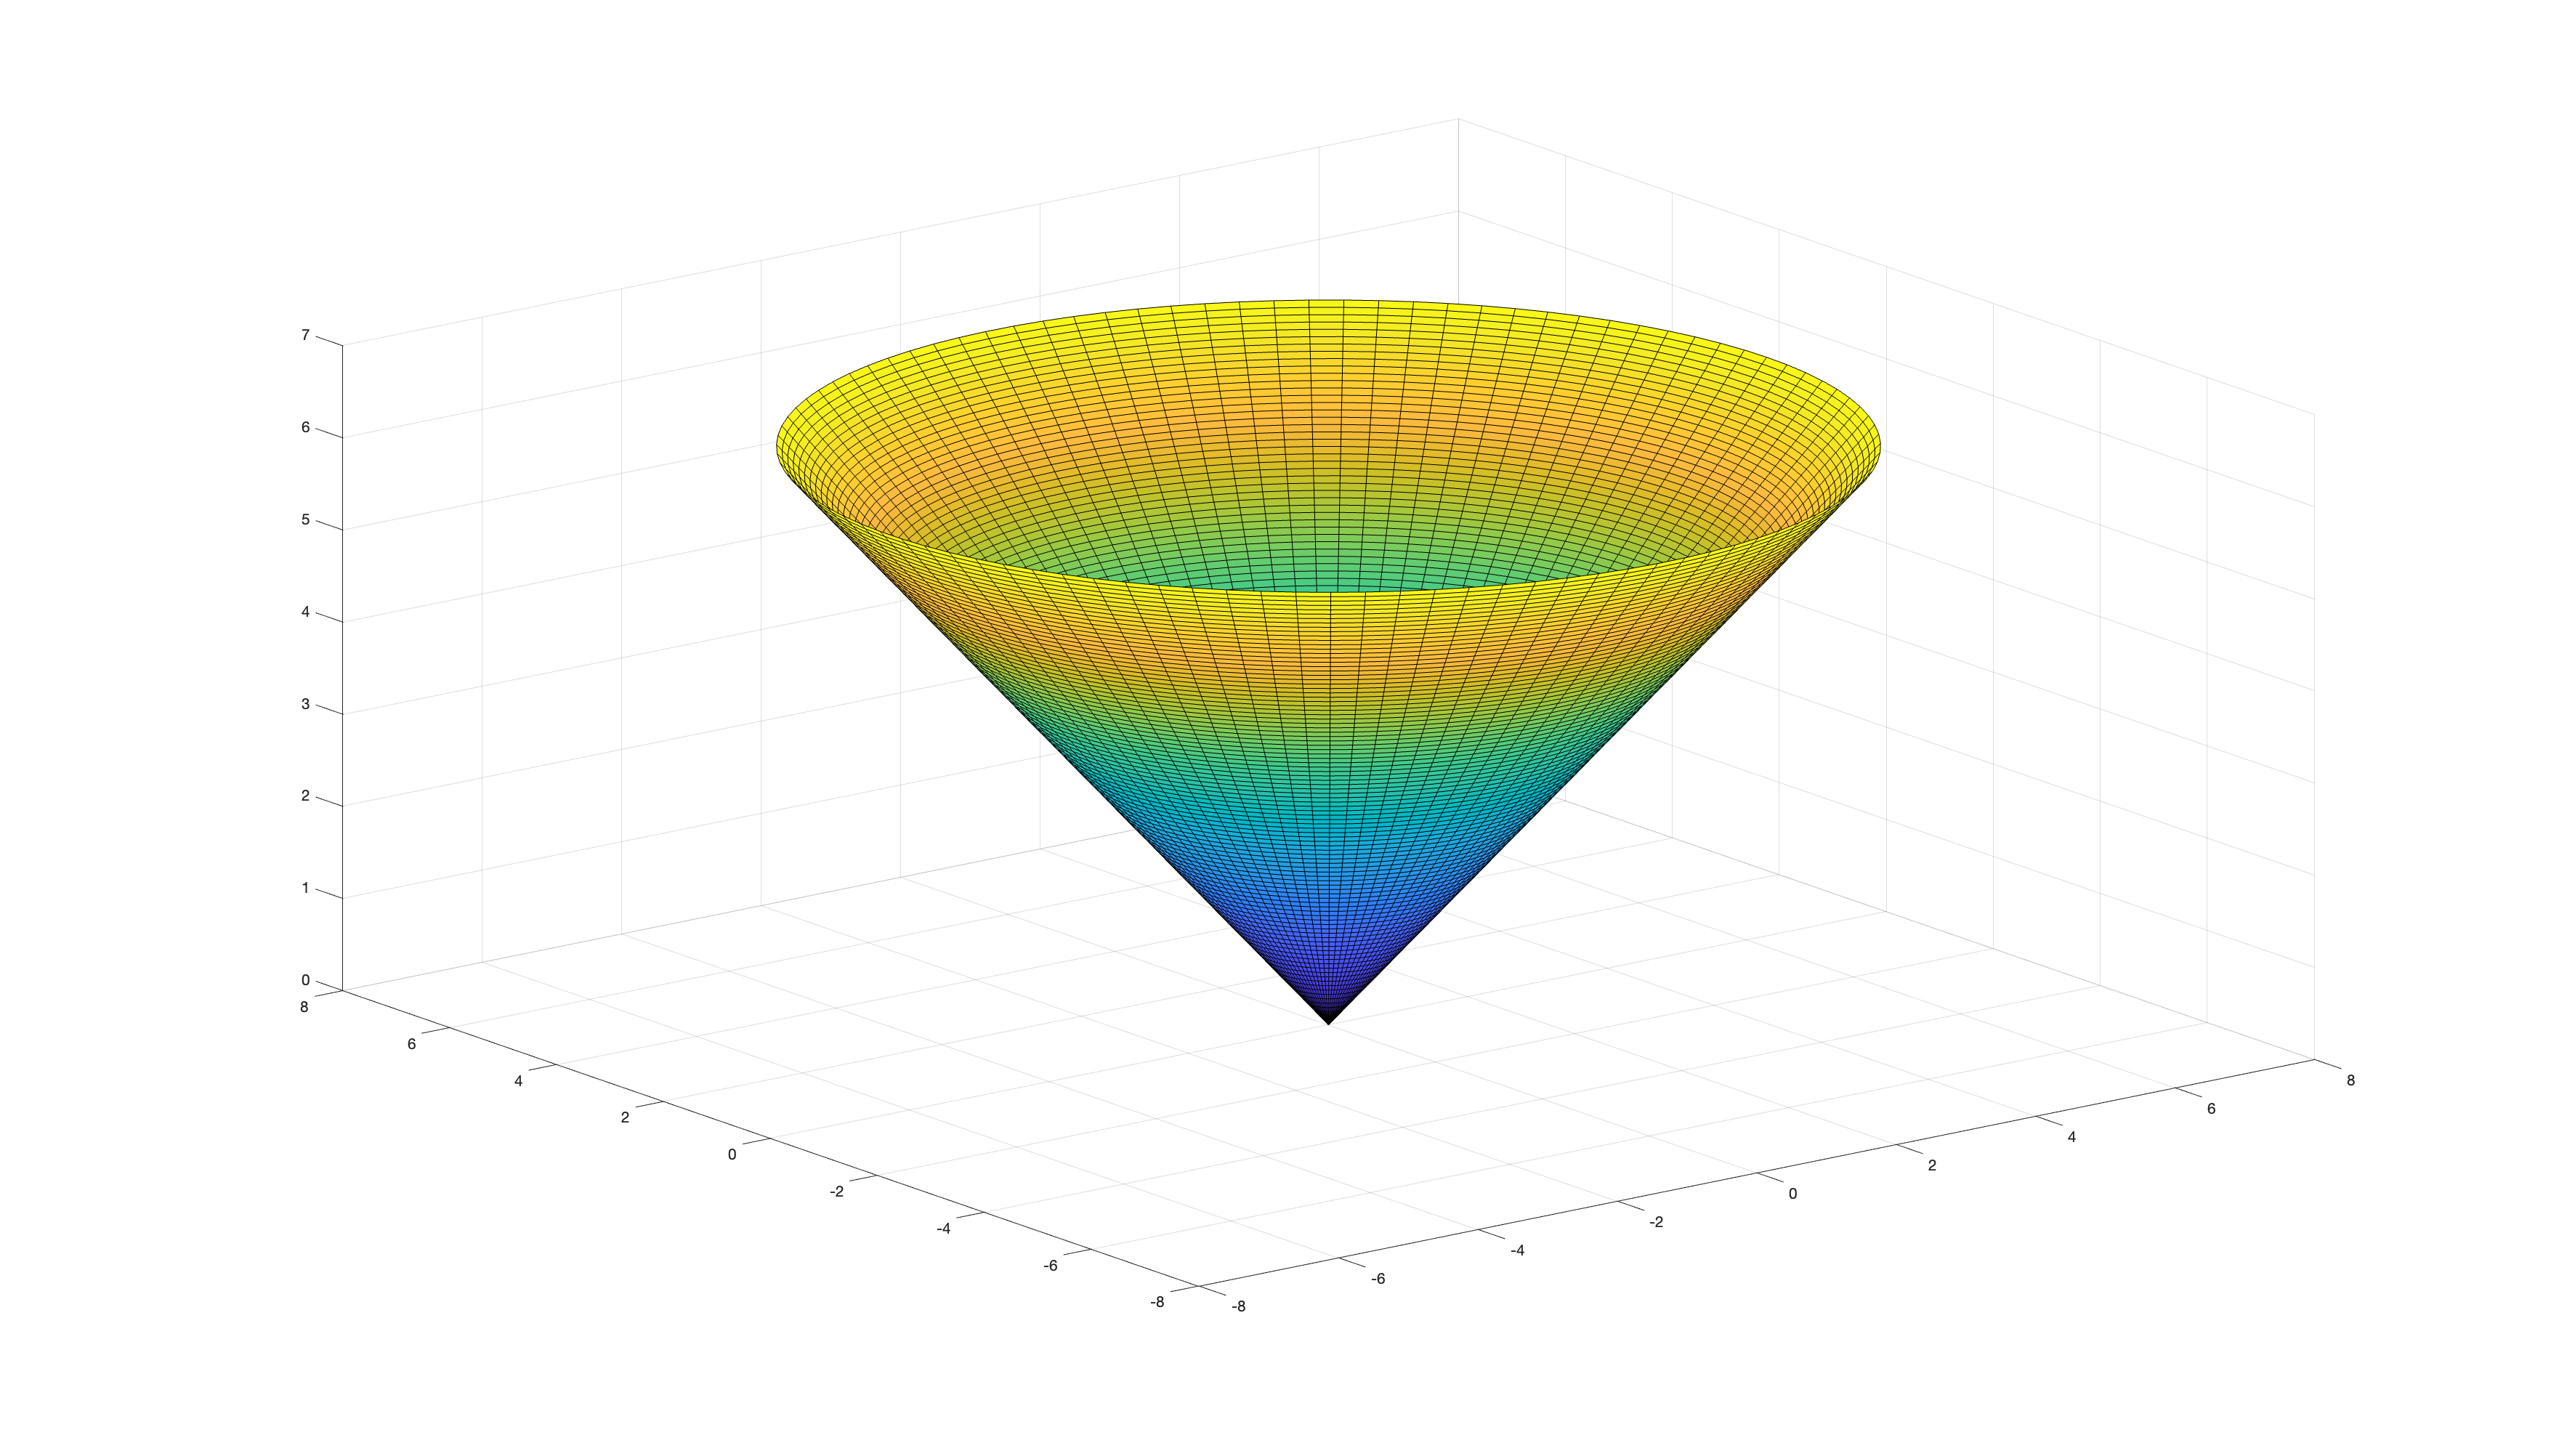
\includegraphics[width=8cm]{img/finiti/cono.eps}
			\caption{Rappresentazione grafica della conica}
			\label{fig:conica}
		\end{figure}
		\begin{equation*}
			\nabla f=0
			\begin{cases}
				z_x=\frac{x}{\sqrt{x^2+y^2}}\\
				z_y=\frac{y}{\sqrt{x^2+y^2}}
			\end{cases}\begin{cases}
					x=0\\
					y=0
			\end{cases} 
		\end{equation*}
		  \begin{nota}
			  sarebbe (0,0) ma il dominio delle derivate $x^2+y^2>0$ cioè
			  $\forall(x,y)\in R^2-\{0,0\}$ in (0,0) non è derivabile.
		  \end{nota}
		  Sappiamo\footnote{si vede geometricamente} che in (0,0) c'è un
		  {\color{red}minimo assoluto}
	  \item $z=x^4 +y^4$
		  \begin{equation*}
			\begin{cases}
				z_x=4x^3=0\\
				z_y=
			\end{cases}\begin{cases}
					x=0\\
					y=0
			\end{cases} \text{ in (0,0) può esserci Max/Min relativo}
		  \end{equation*}
		  \begin{equation*}
			  \begin{matrix}
				det H=\begin{vmatrix}
					0 & 0\\
					0 & 0
				\end{vmatrix} = 0 & \begin{matrix}
					f_{xx}(0,0)=12x^2|_{0,0}=0\\
					f_{xx}(0,0)= 0\\
					f_{yy}(0,0)=12y^2|_{0,0}=0
				  \end{matrix}
			  \end{matrix}
		  \end{equation*}
		  $det H=0 \to$ non so se in (0,0) c'è un massimo o un minimo
		  relativo.\\
		  Per definire se esiste un massimo o un minimo relativo uso:
		  \begin{equation*}
			  \begin{matrix}
				  \min f(x_0,y_0)\leq f(x,y) & 0\leq x^4+y^4 & x^4+y^4\geq 0 &
				  \text{ \underline{SI} $\forall(x,y)$ risulta da
				  $x^4+y^4\geq 0 (0,0)\min$}\\
				  \max f(x_0,y_0)\geq f(x,y) & 0\geq x^4+y^4 & x^4+y^4\leq 0 &
				  \text{ \underline{NO}}
			  \end{matrix}
		  \end{equation*}
  \end{enumerate}
\end{esempio}
\subsection{Ricerca del massimo e del minimo assoluti}
Condizioni sufficienti per l'essistenza del Massimo e del minimo assoluto
\subsubsection{Teorema di Weierstrass}
\begin{teorema}
	Sia f(x,y) definita in D, i continua in D chiuso e limitato, allora il
	minimo e massimo assoluto in D.
	\begin{multicols}{2}
		\paragraph{Ipotesi:}
		\begin{equation*}
			f\in C^0_D
		\end{equation*}
		D chiuso e limitato
		\paragraph{Tesi:}
		$\exists\min$ con $m=f(x_1,y_1), M=f(x_2,y_2)$ tale che $m\leq
		f(x,y)\leq M$
	\end{multicols}
	\paragraph{Ricerca dei punti di Massimo e minimo assoluti:}
	\begin{itemize}
		\item nei punti di massimo o minimo relativo;
		\item nei punti di non derivabilità;
		\item nei punti di frontiera.
	\end{itemize}
	Vanno ricercati quindi nei seguenti modi:
	\begin{enumerate}
		\item $\nabla f=0$ dove il gradiente si annulla;
		\item $\exists \nabla f$ dove il gradiente non esite;
		\item sulla FD sulla frontiera.
	\end{enumerate}
\end{teorema}
\subsubsection{Studio sulla frontiera}
Sia $\xi$ una superficie definita in un insieme D e sia FD la mia frontiera\\
La frontiera FD è una curva\footnote{o insieme di curve} e suoi punti linitano
l'iperbole $\xi$.\\
Possiamo definire la frontiera in forma parametrica
\begin{equation*}
	FD:\begin{cases}
		x=x(t)\\
		y=y(t)
	\end{cases} t\in [a,b] \mathds{R}\to \mathds{R}^2
\end{equation*}
Calcolo la funzione $f(x,y)$ sui punti della frontiera
\begin{equation}
	f(x,y)\to F(t)=f(x(t),y(t))\text{ funzione di 1 variabile}
\end{equation}
studio del massimo e minimo per $F(t)=0\begin{cases}
	F^{\prime\prime}>0 \min\\
	F^{\prime\prime}<0 \max
\end{cases}$\\
Calcolo i valori della funzione nei punti di Massimo/minimo e li confronto con
i valori Massimo/minimo relativi nel dominio e i valori nei punti di non
derivabilità. La frontiera può anche essere in forma cartesiana
\begin{equation}
	\begin{matrix}
		y=y(x) & a\leq x\leq b
	\end{matrix}
\end{equation}
Calcolo la funzione nei punti della frontiera e procedo come visto prima
$f(x,y)\to F(t)=f(x(t),y(t))$
\begin{esempio}
	Determinare il massimo e il mino assoluto di $f(x,y)=
	1+2x^2+\sqrt{x^2+y^2}$ in $D:\{x^2+y^2\leq \Delta\}$
	\begin{enumerate}
		\item $\nabla f=0$
		\item $\nexists \nabla f$
		\item $FD$
	\end{enumerate}
	\begin{enumerate}
		\item $\nabla f(x,y)=0\begin{cases}
				f_x=0\\
				f_y=0
		\end{cases}\begin{cases}
			4x+\frac{x}{\sqrt{x^2+y^2}}\\
			\frac{y}{\sqrt{x^2+y^2}}
		\end{cases}\begin{cases}
			4x+\frac{x}{\abs x}=0\\
			y=0
		\end{cases}$
		\begin{equation*}
			\begin{cases}
				x=0\\
				y=0
			\end{cases}
		\end{equation*}
			$\nabla f=0$ in (0,0) che non è nel C.E. delle derivate parziali
			per cui $\nabla f \neq 0$ $\forall (x,y)\in A$ A dominio $f_x$ e
			$f_y$
		\item $\nexists \nabla f$ le derivate parziali perime sono definite
			$\forall (x,y)\in R^2:x^2+y^2\neq 0$ cioè in $R^2-\{0,0\}$
			\begin{equation*}
				(0,0) \text{ pnto di non derivabilità } f(0,0)=1
			\end{equation*}
		\item FD
			\begin{equation*}
				\begin{matrix}
					D:\{x^2+y^2\leq 4\} & FD: x^2+y^2=4\\
					& \begin{cases}
						x=2\cos t \\
						y=2\sin t
					\end{cases} t\in [0;2\pi]
				\end{matrix}
			\end{equation*}
			Calcolo $f(x,y)$ sui punti di frontiera
			\begin{equation*}
				f(x,y)=F(t)=1+2(2\cos t)^2+\sqrt{(2\cos t)^2+(2\sin t)^2} =
				1+8\cos^2t+2 = 3+8\cos^2t
			\end{equation*}
			Calcolo $F(t)$ agli estremi $t\in[0;2\pi]$ $F(0)=3+8=11$
			$F(2\pi)=3+8=11$\\
			Studio del massimo e del minimo di $F(t)$
			\begin{equation*}
				\begin{matrix}
					F^\prime(t)=0 & 16\cos t(\sin t)=-16\sin t\cos t =0 & t=0&
					t=\pi & t=\frac{\pi}{2}t=\frac{3}{2} \pi
				\end{matrix}
			\end{equation*}
			\begin{equation*}
				F^{\prime\prime}(t)=16(\cos t \cos t -\sin t \sin t) =16(\sin^2
				t- \cos^2 t)
			\end{equation*}
			\begin{equation*}
				\begin{matrix}
					\text{Ottenuti mettendo a F(t) e valori}\\
					\text{dove ci dovrebbero essere un}\\
					\text{massimo e un minimo}
				\end{matrix} \begin{cases}
					F^{\prime\prime}(\pi)=16(-1)=-16<0\text{ }\max\text{ su FD
					}&
					F(\pi) =3+8=11\\
					F^{\prime\prime}(\frac{\pi}{2})=16(-1)=-16>0\text{
					}\min\text{ su
					FD }& F(\frac{\pi}{2}) =3\\
					F^{\prime\prime}(\frac{3\pi}{2})=16(-1)=-16<0\text{
					}\min\text{ su
					FD }& F(\frac{3\pi}{2}) =3
				\end{cases}
			\end{equation*}
	\end{enumerate}
	Ho ottenuto i sequenti valori
	\begin{equation*}
		\begin{matrix}
			1.\text{ }(x,y) \equiv (0,0) & \text{il }\min \text{ è 1 e viene assunto in
			(0,0)} \\
			11.\text{ }t=0,\pi,2\pi & \text{il } \max \text{ è 11 e viene
			assunti in }&
			\begin{cases}
				x=2\cos 0\\
				y=2\sin 0
			\end{cases}\\
			3.\text{ }t=\frac{\pi}{2}, \frac{3}{2}\pi & \begin{cases}
				x=2\cos \pi \\
				y=2\sin \pi
			\end{cases} & (-2,0) & \begin{cases}
				x=2\cos 2\pi \\
				y=2\sin 2\pi
			\end{cases} & (2,0)
		\end{matrix}
	\end{equation*}
\end{esempio}
\subsection{Metodo dei moltiplicatori di di Lagrange}
Nel caso in cui $g(x,y)=0$ non definisca una funzione implicata, per trovare i
massimi e minimi vincolati si introduce una funzione ausiliaria, detta
\underline{\color{red}lagrangiana}, così definita:
\begin{equation}
	F(x,y,\lambda)=f(x,y)+\lambda g(x,y)
\end{equation}
$F(x,y,\lambda)$ è combinazione lineare delle funzioni $f(x,y)$ E $g(x,y)$ --
Il parametro $\lambda$ prende il nome di {\color{red}Moltiplicatore di
Lagrange}. I punti di massimo vincolati sono quelli in cui il gradiente di
$F(x,y,z)$ si annulla ovvero\dots
\begin{equation}
	\nabla F_{(x,y,z)}=0 \begin{cases}
		F_x=fx(x,y)+\lambda g_x(x,y)\\
		F_y=fx(x,y)+\lambda g_y(x,y)\\
		F_\lambda=g(x,y)=0
	\end{cases}
\end{equation}
Si risolve questo sistema di tre equazioni in tre variabili e il valore massimo
della funzione è calcolata nei punti soluzioni è il massimo calcolato e il
valore minimo della funzione calcolata nei punti soluzione è il massimo
vincolato.

\chapter{Integrali Doppi e tripli}
\section{Domini normali (semplici)}
\begin{defi}
	I domini delle funzioni a più variabili possono presentare una forma di
	regolarità per cui è possibile delimitare la regione da intervalli e grafici
	di funzione. Si parla quindi di dominio semplice o normale rispetto alla
	variabile delimitabile da un intervallo. La normalità di un dominio è molto
	importante in molte definizioni di integrale multiplo e della sua
	risoluzione tramite le formule di riduzione. Inoltre la presenza di un
	dominio regolare permette ulteriori teoremi e formule d'integrazione, come
	le formule di Gauss-Green, il teorema della divergenza e il teorema del
	rotore.
\end{defi}
\subsection{Dominio normale rispetto all'asse $x$}
Il dominio A si definisce {\color{red} normale} rispetto all'asse $x$ se è così
definito:
\begin{equation}
	A=\begin{cases}
		a\leq x\leq b & x \text{ valria in un intervallo}\\
		g_1(x)\leq y\leq g_2(x) & y \text{ varia tra due funzioni di }x
	\end{cases}
\end{equation}
\begin{esempio}
\begin{equation*}
	D=\begin{cases}
		0\leq x\leq 1\\
		x^2\leq y\leq x
	\end{cases}
\end{equation*}
\end{esempio}
Il dominio $B$ si definisce {\color{red} normale} rispetto all'asse $x$ se è così
definito:
\begin{equation}
	A=\begin{cases}
		c\leq y\leq d & y \text{ valria in un intervallo}\\
		h_1(y)\leq x\leq h_2(y) & x \text{ varia tra due funzioni di }y
	\end{cases}
\end{equation}
\begin{esempio}
\begin{equation*}
	D=\begin{cases}
		0\leq y\leq 1\\
		y< x< \sqrt{y}
	\end{cases}
\end{equation*}
\end{esempio}
\subsection{Domini Polarmente normale}
Il dominio C si definisce polarmente normale se è costantemente definito:
\begin{equation}
	C=\begin{cases}
		\theta_1\leq \theta\leq \theta_2 \\
		\varphi_1(\theta)\leq \varphi(\theta)\leq \varphi_2(\theta)
	\end{cases}
\end{equation}
\begin{esempio}
  \begin{equation}
    (x-1)^2+y^2\leq 1
  \end{equation}
  l'angolo varia tra 0 e $\frac{\pi}{2}$, il segmento $\varphi$ dipende dall'angolo
  \begin{equation*}
    \begin{matrix}
      \theta=0\text{ è } \max \varphi=2 \\
      \theta=\frac{\pi}{2} \text{ è } \min \varphi=0 \\
      \varphi=2\cos \theta
      \begin{cases}
        0\leq \theta \leq \frac{\pi}{2}\\
        0\leq \varphi\leq 2\cos \theta
      \end{cases}
    \end{matrix}
  \end{equation*}
  corona circolare $\varphi=r$ $\varphi=R$
  \begin{equation*}
    \begin{cases}
      0\leq \theta \leq \frac{\pi}{2}\\
      r\leq \varphi\leq R
    \end{cases}
  \end{equation*}
\end{esempio}
\subsection{Definizione di integrale doppio}
\begin{defi}
  Sia f(x,y) una funzione limitata nel rettangolo $R=[a,b]x[c,d]$, coordinata in $[a,b]$ e
  di seconda coordinata in $[c,d]$
  Deconpongo regolarmante gli intervalli $[a,b]$ e $[c,d]$,
  \begin{equation*}
    \begin{matrix}
        \text{decomponendo }[a,b]\text{ si ha} & D_1=\{x_0=a,x_1,x_2,\dots,x_n=b\}\\ 
        \text{decomponendo }[c,d]\text{ si ha} & D_1=\{y_0=a,y_1,y_2,\dots,y_n=d\}
    \end{matrix}
  \end{equation*}
  Il prodotto cartesiano $D=D_1*D_2$ è una semidivisione del rettangolo R
  \begin{figure}[ht]
    \centering
    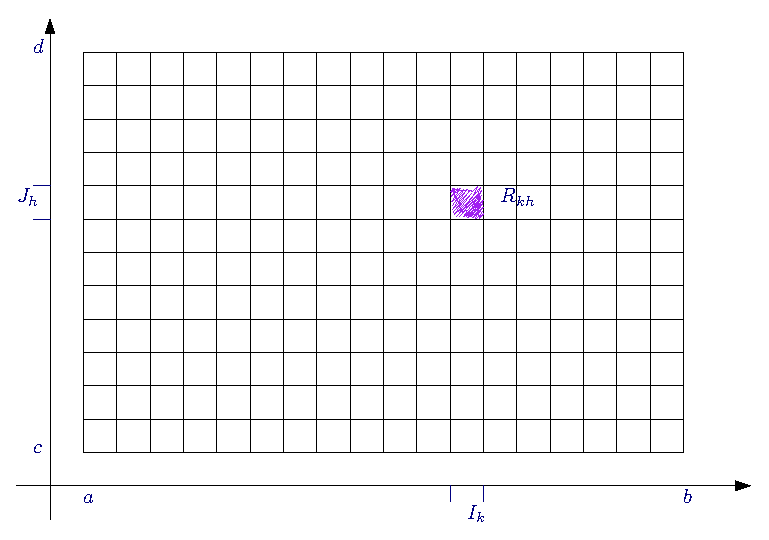
\includegraphics[width=8cm]{img/finiti/graficodecomposizioneR.eps}
    \caption{Decomposizione del rettangolo R}
  \end{figure}
  \begin{equation*}
    \begin{matrix}
        I_k=[x_{k-1},x_k] \text{ in } D_1 (k=1,\dots,n)\\
        J_h=[y_{h-1},y_h] \text{ in } D_2 (h=1,\dots,n)
    \end{matrix}
  \end{equation*}
  Il prodotto cartesiano $I_k*J_h$ individua il generico subrettangolo $R_{kh}$ della semidivisione.\\
  Prendo un generico punto del subrettangolo $R_{kh}(x_k,y_h)$ e faccio il seguente prodotto:
  \begin{equation*}
    f(x_k,y_h)*mis R_{kh} \text{ con } misR_{kh} = misI_k * misJ_h \text{ area del subrettangolo}
  \end{equation*}
  Con l'integrale doppio consudero il volume del parallelepipedo.\\
  Geometricamente considera il pettangolo $R_{kh}$ e la parte di superficie $f(x,y)$ che vi si
  presenta il prodotto $f(x_i,y_n)*mis R_{kh}$ è il volume del parallelepipedo di base $R_{kh}$
  e altezza $f(x_k,y_h)$.
\end{defi}
\section{Somme di Riemann}
Definisco le somme di Riemann $\displaystyle\sum^{k=m\text{ } h=n}_{k=h=1}f(x_k,y_h)*R_{kh}$ ciò
rappresenta la somma di tutti i volumi dei parallelepipedi di base $R_{kh}$ e altezza $f(x_k,y_h)$
che si possono ottenere nel rettangolo $R$.\\
Infittisco le decomposizioni $D_1$ e $D_2(m\to \infty;n\to\infty)$, ottenendo così un numero sempre
maggiore di subrettangoli di ampiezza via via minore.
\begin{equation}
  mis R_{kn}=misI_k*misI_n=\frac{b-a}{m} * \frac{d-c}{n}\to 0 \text{ per }  m,n \to \infty
\end{equation}
Con l'infittirsi della decomposizione, aumenta la precisione con cui ciascun parallelepipedo
approssima il volume sotto al grafico delle funzione in ogni $R_{kh}$.\\
Al limite, le somme di Riemann daranno il volume sotto al grafico della funzione in un certo
rettangolo (in generale dominio).\\
Se esiste finito $\lim\limits_{n\to \infty\text{ } m\to \infty}\displaystyle\sum_{h=k=1}^{k=m\text{ }h=n}f(x_k.y_n)*misR_{kh}$ tale limite è definito \underline{\color{red} ingrale doppio} di f(x,y) nel
dominio $R=[a,b]*[c,d]$
\begin{equation}
  \iint_R f(x,y)dxdy=\lim\limits_{n\to \infty\text{ } m\to \infty}\displaystyle\sum_{h=k=1}^{k=m\text{ }h=n}f(x_k.y_n)*misR_{kh}
\end{equation}
\paragraph{Somme superiori e somme inferiori}
\begin{defi}
  È possibile definire l'integrale doppio anche con le somme superiori e le somme inferiori
  \begin{equation*}
    \text{Somme inferiori } s(f,R) = \displaystyle\sum inf_{R_{kh}}f(x_k.y_n)*misR_{kh}
  \end{equation*}
  prendo il minimo valore che la funzione assume nel subrettangolo $R_{kh}$ e lo moltiplico per
  l'area di tale subrettangolo. Sommando ottengo un parallelepipedo, il cui volume approssima
  per difetto individuato dalla funzione. 
  \begin{equation*}
    \text{Somme superiori } s(f,R) = \displaystyle\sum sup_{R_{kh}}f(x_k.y_n)*misR_{kh}
  \end{equation*}
  prendo il massimo valore che la funzione assume nel subrettangolo $R_{kh}$ e lo moltiplico per
  l'area di tale subrettangolo. Sommando ottengo un parallelepipedo, il cui volume approssima per
  eccesso quello individuato dalla funzione all'infittirsi della decomposizione le somme inferiori
  crescono, le somme superiori decrescono. Le somme superiori e le somme inferiori convergono ad
  uno stesso valore, detto {\color{red}integrale doppio}\footnote{è il valore sotto al grafico
    della funzione}
  \begin{equation*}
    \lim s=\lim S=\iint_R f(x,y)dxdy
  \end{equation*}
\end{defi}
\clearpage
\subsection{Proprietà dell'integrale doppio}
\begin{equation*}
  \begin{matrix}
  \text{Linearità } \begin{cases}
                      1) \iint_D [f_1(x,y)+f_2(x,y)]dxdy=\iint_Df_1(x,y)dx*dy+\iint_Df_2(x,y)dx*dy\\
                      2) \iint_D \alpha f_1(x,y)dxdy=\alpha\iint_Df_2(x,y)dx*dy
                    \end{cases}\\
    \text{Assitività } 3)\text{ Sia } D=D_1\cup D_2 \iint_Df(x,y)dxdy=\iint_{D_1}f(x,y)dx*dy +\iint_{D_2}f(x,y)dx*dy\\
    \text{Monotonia } \begin{cases}
                        4) \text{ Sia } f(x,y)\leq g(x,y)\text{ } \forall (x,y) \in D\\
                        \text{ }\iint_Df(x,y)dxdy \leq \iint_Dg(x,y)dx*dy\\
                        5) \text{ Sia } D_1 \subset D\\
                        \text{ } \iint_{D_1}f(x,y)dxdy < \iint_Df(x,y)dx*dy \\
                        6) \abs{\iint_Df(x,y)dxdy} \leq \iint_D\abs{f(x,y)}dx*dy
                      \end{cases}
  \end{matrix}
\end{equation*} 

\subsection{Formula di riduzione}
\begin{itemize}
\item Sia $A\subset R^2$ un dominio normale rispetto all'asse x
  \begin{equation*}
    A=\begin{cases}
        a\leq x\leq b\\
        g_1(x)\leq y\leq g_2(x)
      \end{cases}
  \end{equation*}
    Allora $\iint_A f(x,y) dxdy=\int_a^bdx \left(\int_{g_1(x)}^{g_2(x)}f(x,y)dy\right)$\\
    calcolo prima $\int_{g_1(x)}^{g_2(x)}f(x,y)dy$ che è una funzione della sola $x$ $\not{o}(x)$
    \begin{equation*}
      \text{per calcolo } \int^b_a \not{o} (x) dx
    \end{equation*}
  \item Dominio polarmente normale\\
    Effettua un cambio di coordinate, passando dalle coordinate cartesiane a quelle polari
    \begin{equation*}
      \text{L'integrale doppio è } \iint_Df(x,y)dxdy
    \end{equation*}
    Passando alle coordinate polari
    \begin{equation*}
      \begin{matrix}
        \text{del dominio } D(x,y) \text{ passerò al dominio } D^\prime (\varphi, \theta) \\
        \text{della funzione } f(x,y) \text{ passerò al dominio } f (\varphi, \theta)
      \end{matrix} \begin{cases}
                       x=\varphi\cos\theta\\
                     y=\varphi\sin\theta
                   \end{cases}
                   \varphi=\sqrt{x^2+y^2} 
   \end{equation*}
   e da differenziali $dxdy$ passerò ai differenziali $d\varphi d\theta$. \\
   Si dimostra che nel passaggio ad altre coordinate il differenziale è $\abs{j} d\varphi d\theta$,
   dove $\abs j$ è il determinante della {\color{red} matrice Jacobiana} che contiene le derivate
   parziale prime
   \begin{equation}
     \abs{J}=\begin{vmatrix}
               x_\varphi & x_\theta\\
               y_\varphi & y_\theta
             \end{vmatrix}
             \to \abs{J}=\begin{vmatrix}
                           \cos \theta & -\varphi \sin \theta\\
                           \sin \theta & \varphi \cos \theta
                         \end{vmatrix}
                         =\varphi\cos^2\theta+\varphi \sin^2\theta =\varphi
   \end{equation} 
   Per cui passando da $dxdy$ alle coordinate polari avrò $\varphi d\varphi d\theta$ così
   l'integrale doppio diventa:
   \begin{equation*}
     \iint_Df(x,y)dxdy=\iint_{D^\prime}f(\varphi,\theta)\varphi d\varphi d\theta
   \end{equation*}
\end{itemize}
\clearpage
\subsubsection{Esempi di domini polarmente normali}
\begin{figure}[ht]
  \centering
  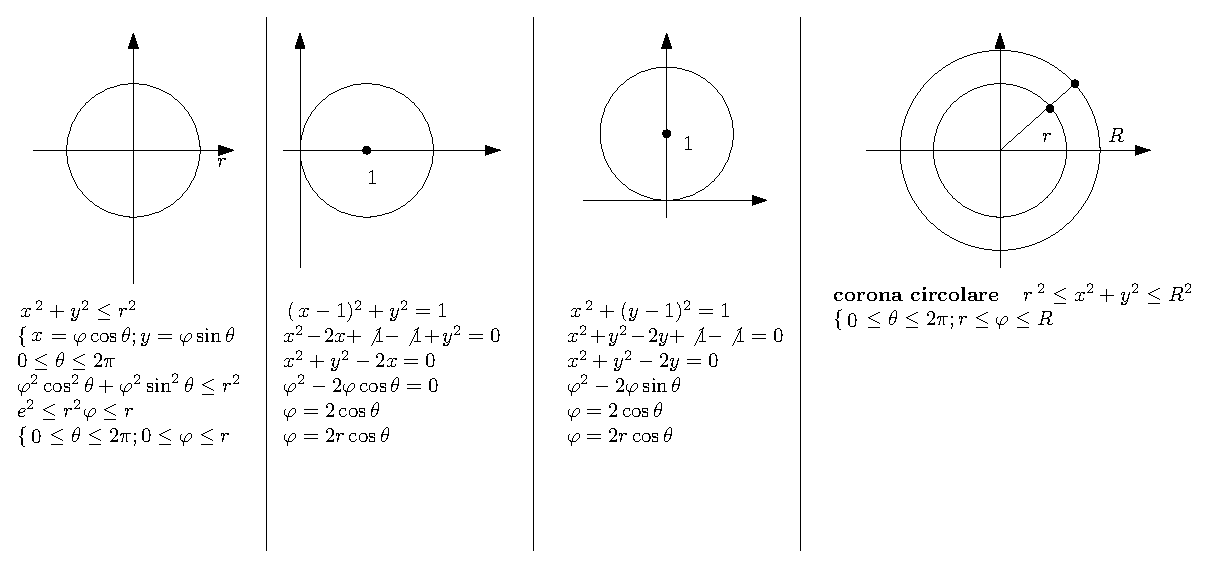
\includegraphics[width=14cm]{img/finiti/esdompolnorm.eps}
  \caption{Esempi di domini polarmente normali}
\end{figure}
\subsection{Baricentro di un dominio normale}
\begin{defi}
  Sia D un demonio normale del piano. Si definisce {\color{red}baricentro del dominio} D il punto di
  coordinate $(x_0,y_0)$ tale che:
  \begin{equation*}
    \begin{matrix}
      x_0=\frac{1}{mis D} \iint_D xdxdy & y_0=\frac{1}{mis D} \iint_D ydxdy
    \end{matrix}
  \end{equation*}
  $mis D:$ misura ({\tt area}) del dominio $D$.
\end{defi}
\begin{esempio}
  calcolare il baricertro del dominio $D=\begin{cases}
                                           0\leq x\leq 2\\
                                           0\leq y\leq 1
                                         \end{cases}$
  \begin{equation*}
    mis D=A_{rettangolo}=2*1=2
  \end{equation*}
  \begin{figure}[ht]
    \centering
    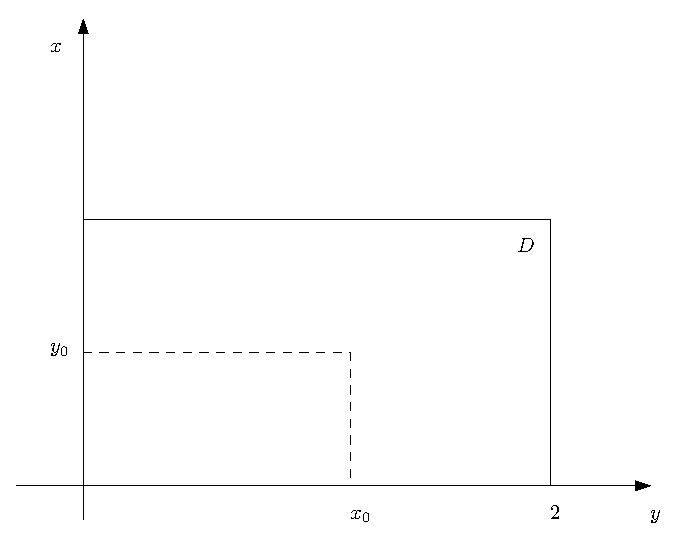
\includegraphics[width=6cm]{img/finiti/baricentrodiundominionormale.eps}
    \caption{Baricentro di un dominio normale}
  \end{figure}
  \begin{equation*}
    \begin{matrix}
      x_0=\frac{1}{mis D}\iint_D xdxdy=\frac{1}{2}\int_0^2dx\int_0^1xdy=\frac{1}{2}\int^2_0dx\abs{xy}_0^1= \frac{1}{2}\int_0^2xdx=\frac{1}{2}\abs{\frac{x^2}{2}}_0^2=\frac{1}{\not{2}}\not{2}=1\\
      y_0=\frac{1}{mis D}\iint_D ydxdy=\frac{1}{2}\int_0^2dx\int_0^1ydy=\frac{1}{2}\int_0^2dx\left|\frac{y^2}{2}\right|^1_0=\frac{1}{2}\int^2_0\frac{1}{2}dx=\frac{1}{4}\left|x\right|=\frac{1}{2}
    \end{matrix}
  \end{equation*}
  \clearpage
   \begin{center}
            \fbox
            {
            \begin{minipage}{0.85\textwidth}
		Calocolare il baricentro del dominio $D=\begin{cases}
                                                          0\leq \theta \leq \frac{\pi}{2}\\
                                                          0\leq y \leq \sqrt{1-x^2}
                                                          \end{cases}$
              \begin{multicols}{2}
                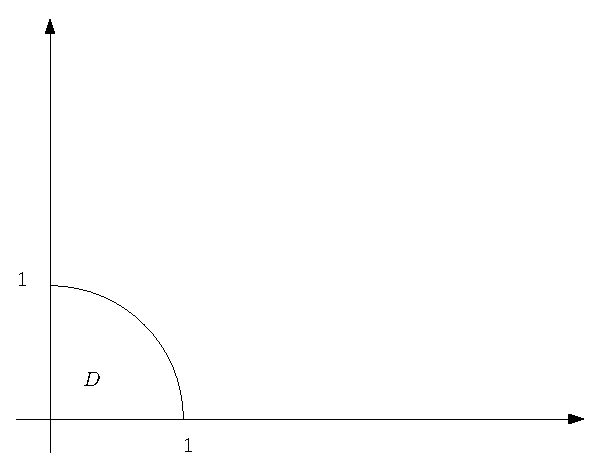
\includegraphics[width=6cm]{img/finiti/baricentrodiundominionormale2.eps}\\
                \begin{equation*}
                  \begin{matrix}
                    D=\begin{cases}
                      0\leq \theta\leq\frac{\pi}{2}\\
                      0\leq \varphi\leq 1
                    \end{cases} & mis D=\frac{\pi}{4}
                  \end{matrix}
                \end{equation*}
              \end{multicols}
              \begin{equation*}
                \begin{matrix}
                  x_0= \frac{1}{mis D}\iint_D xdxdy=\frac{4}{\pi}
                  \int^{\frac{\pi}{2}}_0d\theta\int_0^1
                  \varphi^2\cos \theta d\theta = \frac{4}{\pi} \int_0^{\frac{\pi}{2}}d\theta \left|
                  \frac{\varphi^3}{3}\cos\theta\right|_0^1\\=\frac{4}{\pi}\int_0^{\frac{\pi}{2}}
                  \frac{1}{3} \cos \theta d\theta = \frac{4}{3}\pi \left|\sin
                  \theta\right|^{\frac{\pi}{2}}_0=\frac{4}{3}\pi\\
                  y_0=\frac{1}{mis D}\iint_D xdxdy=\frac{4}{\pi}
                  \int^{\frac{\pi}{2}}_0d\theta\int_0^1
                  \varphi^2\sin \theta d\theta = \frac{4}{\pi} \int_0^{\frac{\pi}{2}}d\theta \left|
                  \frac{\varphi^3}{3}\sin\theta\right|_0^1\\
                  =\frac{4}{\pi}\int_0^{\frac{\pi}{2}}\frac{1}{3}\sin\theta d\theta =\frac{4}{\pi}*
                  \frac{1}{3}\left|-\cos\theta \right|^{\frac{\pi}{2}}_0=\frac{4}{3}\pi
                \end{matrix}
              \end{equation*} 
            \end{minipage}
            }
  \end{center}
\end{esempio}
\subsection{Domini normali in $R^3$}
\begin{defi}
Il dominio $V$ definisce normale rispetto al piano $xy$ se si può così descrivere:
\begin{equation*}
  \begin{matrix}
    \begin{cases}
      (x,y)\in D & \text{normale}\\
      \alpha(x,y) & \leq z\leq \beta (x,y)
    \end{cases}& \begin{matrix}
                   (x,y) \text{ appartengono ad un dominio normale di } R^2\\
                   z \text{ è compresa tra funzioni di } x \text{ e } y 
                 \end{matrix}
  \end{matrix}
\end{equation*}
$\forall (x,y)\in D$ incontro prma la superficie minorante e per la superficie maggiorante.
\end{defi}
\section{Integrali tripli}
\begin{defi}
  Sia $f(x,y,z)$ una funzione limitata in un insieme $V$, considero il parallelepipedo
  \begin{multicols}{2}
    \begin{equation*}
      V=[a,b]*[c,d]*[e,f]
    \end{equation*}
    Decompongo regolarmente $[a,b],[c,d],[e,f]$\\
    rispettivametne in $n,m e k$\\
    intervalli $I_n=[x_0=a,\dots,x_n=b]$,
    \begin{equation*}
      l_m=[y_0=c,\dots,y_m=d],\text{ } l_k=[z_0=e,\dots,z_k=f]
    \end{equation*}
    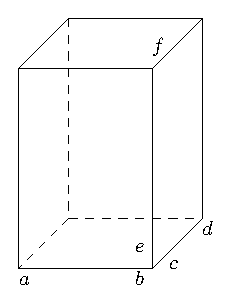
\includegraphics[width=4cm]{img/finiti/rettangolo.eps}
  \end{multicols}
  Il prodotto cartesiano $I_n*I_n*I_k$ individua il generico subparallelepipedo $V_{n,m,k}$.
\end{defi}
\clearpage
Definisco le somme di Riemann: $\sum f(x,y,z)*misV_{n,m,k}$\footnote{$misV_{n,m,k}$: misura il
  volume del parallelepipedo}\\
All'infittirsi delle decomposizioni le somme di Riemann convergono ad uno stezzo valore, tale
valore è definito {\color{red}integrale triplo} di $f(x,y,z)$ in $V$
\begin{equation*}
  \lim_{m\to \infty\text{ } n \to \infty \text{ } k\to \infty}\sum f(x,y,z) misV_{n,m,k}=\iiint_V f(x,y,z)dxdydz
\end{equation*}
Oppure, definisco le somme inferiore e le somme superiori
\begin{equation*}
  \begin{matrix}
    \text{Somme inferiori} &\sum misV_{n,m,k}*\min_{V_{n,m,k}}f(x,y,z)\\
    \text{Somme superiori} &\sum misV_{n,m,k}*\max_{V_{n,m,k}}f(x,y,z)
  \end{matrix}
\end{equation*}
All'infittirsi della decomposizione le somme inferiori crescono mentre le somme superiori
decrescono. Se convergono ad una stesso valore, tale valore è definito {\color{red}integrale triplo}
di $f(x,y,z)$ in $V$
\begin{equation*}
  \lim s(f,V)= \lim S(f,V)= \iint_V f(x,y,z) dxdydz
\end{equation*}
\subsection{Formule di riduzione per gli integrali tripli}
Sia $g(x,y)$ integrabile in un dominio normale $V$
\begin{equation*}
  \begin{matrix}
    V=\begin{cases}
        \alpha (x,y) \leq z\leq \beta (x,y)\\
        (x,y)\in D
      \end{cases} & \iiint_V f(x,y,z) dxdydz = \iint_D dxdy \displaystyle\int_{a(x,y)}^{\beta (x,y)} f(x,y,z)dz
  \end{matrix}
\end{equation*}
Se il dominio $D$ è normale rispetto all'asse $x$
\begin{equation*}
	V=\begin{cases}
		a\leq x\leq b\\
		g_1(x)\leq y\leq g_2(x)\\
		\alpha (x,y) \leq z \leq \beta (x,y)
	\end{cases} \iiint_V f(x,y,z) dxdydz = \int_\theta^\theta dx
	\int_{f_1(x)}^{f_2(x)}dy\int_{\alpha(x,y)}^{\beta(x,y)}f(x,y,z)dz
\end{equation*}
Se il dominio $D$ è normale rispetto all'asse $y$
\begin{equation*}
	V=\begin{cases}
		c\leq y \leq d\\
		h_1(y)\leq x \leq h_2(y)\\
		\alpha (x,y) \leq z \leq \beta(x,y)
	\end{cases} \iiint_V f(x,y,z) dxdydz = \int_c^d dy
	\int_{h_1(y)}^{h_2(y)}\int_{a(x,y)}^{\beta(x,y)} f(x,y,z) dz
\end{equation*}
Se il dominio $D$ è polarmente normale
\begin{equation*}
	V=\begin{cases}
		\theta_1\leq \theta \leq \theta_2\\
		\varphi_1(\theta)\leq \varphi \leq \varphi_2(\theta)\\
		\alpha (\varphi,\theta)\leq z \leq \beta(\varphi,\theta)
	\end{cases} \iiint_V f(x,y,z)dxdydz=\int_{\theta_1}^{\theta_2}d\theta
	\int^{\varphi_2(\theta)}_{\varphi_1(\theta)} \varphi d \varphi
	\int^{\beta(\varphi, \theta)}_{\alpha (\varphi,\theta)}
	f(\varphi,\theta,z)dz 
\end{equation*}
\begin{equation*}
	\begin{matrix}
		\alpha(x,y)&\to&\alpha (\varphi, \theta)\\
		\beta (x,y)&\to& \beta(\varphi, \theta)\\
		f(x,y,z) &\to & f(\varphi,\theta, z)\\
		dxdydz &\to & pd\theta d\varphi dz
	\end{matrix}
\end{equation*}
\clearpage
\subsection{Significato geometrico degli integrali}
\begin{equation*}
	\begin{matrix}
		\int & \text{area}\\
		\iint & \text{volume}\\
		\iiint & \text{nessun significato geometrico}
	\end{matrix}
\end{equation*}
\subsection{Coordinate polari e coordinate cilindriche}
$(x,y) \to (\varphi,\theta)$
\begin{equation*}
	\begin{matrix}
		\begin{cases}
			x=\varphi \cos \theta\\
			y=\varphi \sin \theta
		\end{cases} & \varphi =\sqrt{x^2+y^2} &det J=\varphi
	\end{matrix}
\end{equation*}
\paragraph{coordinate alindriche}
$(x,y,z)\to (\varphi,\theta,z)$
\begin{equation*}
	\begin{matrix}
		\begin{cases}
			x=\varphi \cos \theta\\
			y=\varphi \sin \theta\\
			z=z
		\end{cases} & \varphi =\sqrt{x^2+y^2+z^2} &det J=\varphi
	\end{matrix}
\end{equation*}
\paragraph{coordinate sferiche}
\begin{equation*}
	\begin{matrix}
		\begin{cases}
			x=\varphi \sin\theta \cos \alpha\\
			y=\varphi \sin \theta \sin \alpha\\
			z=\varphi \cos\theta
		\end{cases} 
	\end{matrix}
\end{equation*}
\subsection{Interazione per fette}
Considera un volume $V$ e lo interseco con un piano $z=k$. Così ottengo una
sezione $S_z$
\begin{equation*}
	z=1-x^2-y^2
\end{equation*}
Al variare di $z$ tra due valori, cioè facendo variare $S_z$ in funzione di $z$
descrivo il volume $V$.
\begin{esempio}
	\begin{equation*}
		\int_{0}^{1} S_zdz
	\end{equation*}
	$S_z$ è un cerchio di raggio $R(z)$ che depende da $z$
	\begin{equation*}
		\begin{matrix}
			z=1-x^2+y^2 & x^2+y^2=1-z\\
			R^2=1-z & R(z)=\sqrt{1-z}
		\end{matrix}
	\end{equation*}
	$S_z=\pi R^2=\pi(1-z)$
	\begin{equation*}
		\iint_T f(x,y,z)dxdydz=\int_0^1\pi(1-z)dz
	\end{equation*}
\end{esempio}
\subsection{Integrali curvilinei}
\subsubsection{Curve in $R^2$ e in $R^3$}
\begin{defi}
	Si definisce {\color{red}curva} una coppia del tipo $(\gamma,\Gamma)$ con
	\begin{equation*}
		\vec{F}(t)=(x(t),y(t),z(t),\dots) \text{ } t\in [a,b]
	\end{equation*}
	si tratta di un'applicazione $R\to R^n$ ad un valore di $t$ associo $n$
	valori\\
	Le curve possono essere:
	\begin{itemize}
		\item In forma cartesiana $\begin{matrix}
				z=f(x,y) &(R^3) \\
				y=f(x) &(R^2)
		\end{matrix} \begin{cases}
			x=t\\
			y=f(t)
		\end{cases}$
		\item In forma polare $\begin{matrix}
			\varphi =\varphi(\theta)&\varphi=2r\cos\theta & 0\leq \theta \leq 2\pi
	\end{matrix}$
		\item In forma parametrica $\begin{cases}
			x=x(t)\\
			y=y(t)\\
			z=z(t)
		\end{cases}$
	\end{itemize}
	Nello spazio una curva è l'intersezione tra due superfici.\\
	Ogni curva ha anche un {\color{red}sostegno}, che è il suo grafico nek
	piano o nello spazio.\\
	Una curva si definisce {\color{red}chiusa} se
	\begin{equation*}
		\begin{matrix}
			\vec{F}(t)=\begin{cases}
				x=x(t)\\
				y=y(t)
			\end{cases} & t\in [a,b]\text{ se } \vec{F}(a)=\vec{F}(b) &
			\begin{matrix}
				x(a)=x(b)\\
				y(a)=y(b)
			\end{matrix}
		\end{matrix}
	\end{equation*}
	\begin{figure}[ht]
		\centering
		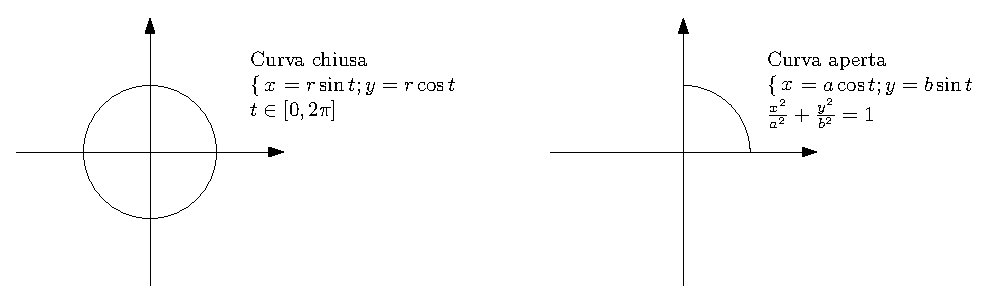
\includegraphics[width=13cm]{img/finiti/curva_chiusa_e_aperta.eps}
		\caption{Differenza tra curva chiusa e aperta}
	\end{figure}\\
	Una curva chiusa la {\color{red}frontiera} di un dominio
	\begin{multicols}{2}
		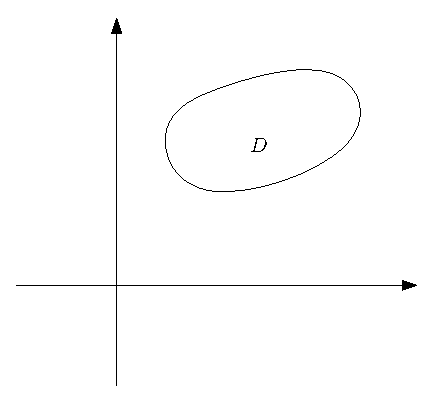
\includegraphics[width=6cm]{img/finiti/dominio.eps}\\
		\begin{equation}
			FD:\begin{cases}
				x=x(t)\\
				y=y(t)
			\end{cases} t\in [a,b]
		\end{equation}
	\end{multicols}
	Una curva si devinisce {\color{red}semplice} se presi due qualunque
	$t_1\neq t_2$ rusylta $\vec{F}(t_1)\neq \vec{F}(t_2)$ cioè 
	\begin{equation*}
		\begin{cases}
			x(t_1)\neq x(t_2)\\
			y(t_1)\neq y(t_2)\\
			z(t_1)\neq z(t_2)
		\end{cases}
	\end{equation*}
	Curva semplice $\gamma \begin{cases}
		x=t\\
		y=\sqrt{t}
	\end{cases} y=\sqrt{x}$ $\gamma \begin{cases}
		x=t\\
		y=t^2
	\end{cases} y=x^2$ Curva non semplice\footnote{$t_1\neq t_2$ ho due stessi
	valori della curva}\\
	Una curva è {\color{red}regolare} se è di classe $c^1$ e le sue derivate
	prime non sono mai nulle contemporaneamente
	\begin{equation*}
		\vec{F}(t)=\begin{cases}
			x=x(t)\\
			y=y(t)\\
			z=z(t)
		\end{cases}
		\begin{matrix}
			\vec{F}(t)\in c^\prime \\
			t\in[a,b]
		\end{matrix}
		r^\prime(t)=(x^\prime,y^\prime,z^\prime(t)\dots)\neq(0,0,0\dots)
	\end{equation*}
	Curva regolare
	\begin{equation*}
		\begin{matrix}
			\gamma z(t)=\begin{cases}
				x=t^3-t\\
				y=t^2-1
			\end{cases} & f\in [-1,1] & z^\prime(t) =\begin{cases}
				x^\prime(t)=3t^2-1\\
				y^\prime(t)=2t
			\end{cases} &\begin{matrix}
				\text{non sono mai nulle}\\
				\text{contemporaneamente}
			\end{matrix}
		\end{matrix}
	\end{equation*}
	\begin{multicols}{2}
		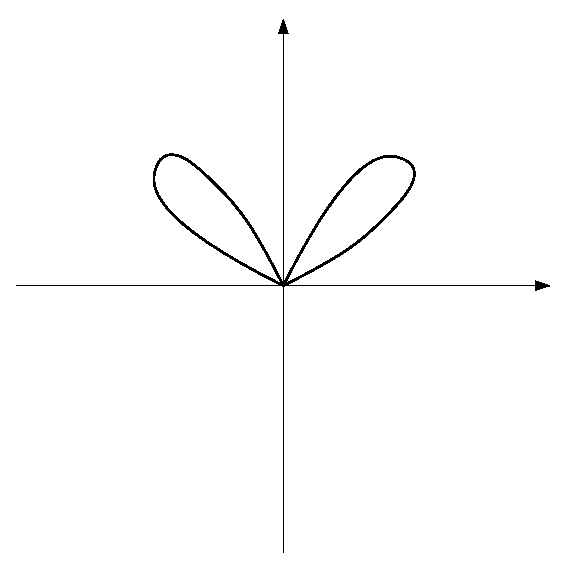
\includegraphics[width=6cm]{img/finiti/curva_regolare.eps}\\
		\begin{equation*}
			r(t)=\begin{cases}
				x=t(1-t^2)^2\\
				y=t^2(1-t^2)
			\end{cases} t\in[-1,1]
		\end{equation*}
	\end{multicols}
	Una curva è {\color{red}regolare a tratti} se è l'unione di curve regolari
	\begin{equation*}
		\gamma r(t)=\begin{cases}
			x=t^3\\
			y=t^2
		\end{cases} t\in[-1,1] \text{ in $x=0$ c'è una cuspide perciò non è regolare $y=\sqrt[3]{x^2}$}
	\end{equation*}
	$r(t)$ può però essere vista come l'unione di che curve regolari
	\begin{equation*}
		\gamma^\prime r (t)=\begin{cases}
			x=t^3\\
			y=t^2
		\end{cases} t\in [-1,0]
	\end{equation*}
	\begin{equation*}
		\gamma^{\prime\prime} r^{\prime\prime}=\begin{cases}
			x=t^3\\
			y=t^2
		\end{cases} t\in [0,1]
	\end{equation*}
	sostegno nel II quadrante
	\begin{equation*}
		\gamma=\gamma^\prime \vee \gamma^{\prime\prime}
	\end{equation*}
\end{defi}
\subsection{Lunghezza di una curva}
\begin{defi}
	Sia la curva $\gamma$ di equazione $\vec{F}(t)$, essa si definisce
	{\color{red}rettificabile} se esiste finito l'estremo superiore della
	poligonale $L(p)$ al variare della decomposizione.
	\begin{equation}
		sup_DL(\Delta)
	\end{equation}
	Suddivido la curva in tanti segmenti che formano la poligonale $L(D)$.
	All'infittirsi la poligonale approssimo sempre seguo la lunghezza della
	curva.\\
	Se la curva $\vec{F}(t)$ è di classe $c^1$ allora essa è
	{\color{red}rettificabile}
	\begin{equation}
		\vec{F}(t)=\begin{cases}
			x=x(t)\\
			y=y(t)\\
			z=z(t)
		\end{cases} t\in [a,b]
	\end{equation}
	e la sua lunghezza vale
	$L=\int_{a}^{b}\sqrt{[x^\prime(t)]^2+[y^\prime(t)]^2 + [z(t)]^2+\dots dt}$
\end{defi}
\subsection{Lunghezza di una curva in forma cartesiana}
Se la curva $\gamma$ nella forma $\begin{cases}
	x=t\\
	y=f(t)
\end{cases} t\in [a,b]$ ha come sostegno il grafico di $y=f(x)$\\
La lunghezza della curva è $L_\gamma=\int_{a}^{b}\sqrt{1+[f^\prime(x)]^2}dx$
\subsection{Lunghezza di una curva polare}
Se le curve è nella forma 
\begin{equation*}
	\begin{cases}
		e=e(\theta)\\
		\theta_1\leq\theta\leq\theta_2
	\end{cases} 
\end{equation*}
La sua lunghezza vale: 
\begin{equation*}
	L_\gamma
	=\int_{\theta_1}^{\theta_2}\sqrt{\varphi^2(\theta)+[\varphi^\prime(\theta)]^2}
	d\theta
\end{equation*}
\section{Ascissa Curvilinea}
È possibile effettuare combiamenti di parametri per descrivere una curva. Fra
tutte le rappresentazioni parametriche di una curva regolare ha particolare
\textbf{importanza} geometrica quella che {\color{red}l'ascissa curvilinea}.
Prendiamo una curva $\gamma$ di $R^2$ e un suo punto $P_0$
\begin{multicols}{2}
	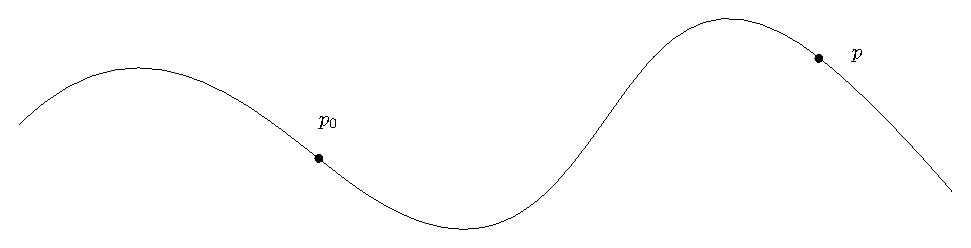
\includegraphics[width=7cm]{img/finiti/ascissa_curvilinea.eps}\\\\\\\\
	Ad ogni punto $P$ della curva associamo un valore $S(P)$ che è uguale
	alla lunguezza dell'arco di curva congiungente $P_0$ e $P$\\
	Così definendo una corrispondenza biurivoca tra i punti della curva e i
	punti di un certo intervallo $[a,b]$, cosiché se $S(p_1)=a$ $S(P_2)=b$ la
	lunqhezza dell'arco congiungente $P_1$ con $P_2$ è $\abs{b-a}$
\end{multicols}
Sia $(\gamma,\vec{r}(t))$ una curva regolare; definiamo \underline{l'ascissa
curvilinea}\footnote{o lunghezza d'arco} come:
\begin{equation*}
	S(t)= \int_{a}^{t}\sqrt{[x^\prime (\uptau)]+[y^\prime(\uptau)]} d\uptau
\end{equation*}
Per il teorema del calcolo integrale
\begin{equation*}
	\begin{matrix}
		S^\prime(t)=\sqrt{[x^\prime(t)]^2+[y^\prime(t)]^2} & S(t) \text{ è
		integrabile}\\
		S^\prime(t)=\frac{ds}{dt} & S:[a,b]\to [0,L]
	\end{matrix}
\end{equation*}
La lunghezza della curva così vale:
\begin{equation}
	L=\int_{a}^{b}\sqrt{[x^\prime(t)]^2+[y^\prime(t)]^2}=\int dS
\end{equation}
\section{Integrale corvilineo}
Prendiamo una funzione f(x,y) definita in un insieme $D$ e una curva $\gamma$
interno a $D$.
\begin{multicols}{2}
	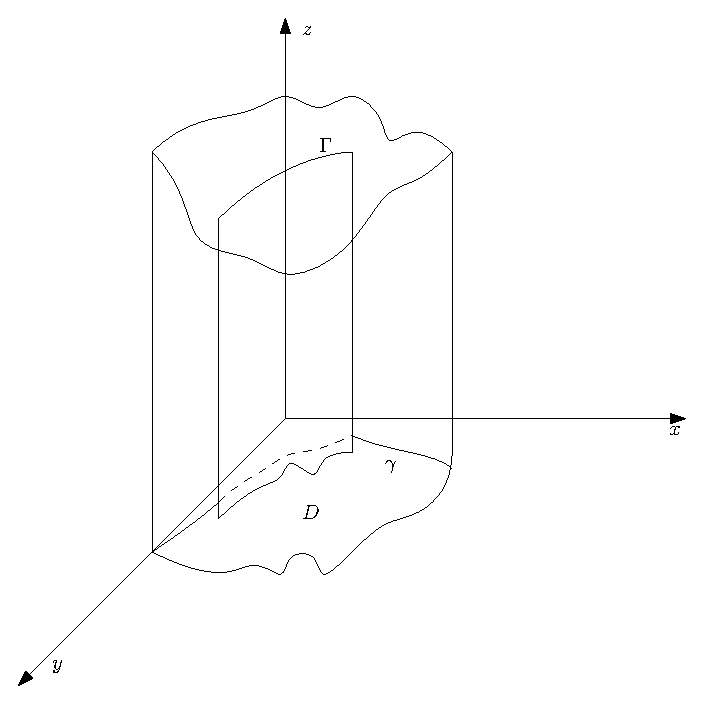
\includegraphics[width=5cm]{img/finiti/integrale_curvilineo.eps}\\
	Calcoliamo la funzione nella curva $\gamma$ e detterminiamo una curva
	$\Gamma$ dello spazio.\\
	L'area delimitata dal cilindro di basi $\gamma$ e $\Gamma$ se $f(x,y)>0$ è
	il valore {\color{red}dell'integrale curvilineo} di $f(x,y)$ esteso a
	$\gamma$.
\end{multicols}
\subsection{Definizione di integrale curvilineo}
Data una curva regolare $(\gamma, \vec{r}(t))$
\begin{equation}
	\begin{cases}
		x=x(t)\\
		y=y(t)\\
		z=z(t)
	\end{cases} t\in [a,b]
\end{equation} 
e una funzione $f(x,y,z)\in \mathds{C}$ -- definita in $D_1$ con la curva
inclusa $D$, si definisce {\color{red}integrale curvilineo} di $f(x,y,z)$
esteso alla curva
\begin{equation*}
	\int_{\gamma} f(x,y,z) ds=
	\int_{a}^{b}f[x(t),y(t),z(t)]*\sqrt{[x^\prime(t)]^2+[y^\prime(t)]^2+[z^\prime(t)]^2}
	dt
\end{equation*}
\subsection{Baricentro di una curva}
Si definisce {\color{red} baricentro di una curva} quel punto di coordinate
$(x_0,y_0)$ per cui
\begin{equation*}
	\begin{matrix}
		x_0=\frac{1}{L_\gamma}\int_\gamma x ds & y_0=\frac{1}{L_\gamma}
		\int_\gamma yds & \text{con $L_\gamma$ lunghezza della curva $\gamma$}
	\end{matrix}
\end{equation*}
\begin{esempio}
	\begin{equation*}
		\gamma=\begin{cases}
			x=\cos^3t\\
			y=\sin^3 t
		\end{cases} t\in \left[0,\frac{\pi}{2}\right]
	\end{equation*}
	\begin{equation*}
		\begin{matrix}
				L_\gamma=\int_{\gamma}ds=\int_{0}^{\frac{\pi}{2}}\sqrt{(-3\cos^2t\sin
			t)^2+(3\sin^2+\cos t)^2} dt\\
			=\int_{0}^{\frac{\pi}{2}}\sqrt{9\cos^4t\sin^2t+9\sin^4t\cos^2t}dt= 
			\int_{0}^{\frac{\pi}{2}}\sqrt{9\cos^2t\sin^2t}*\sqrt{\cos^2t\sin^2t}
			dt = \int_{0}^{\frac{\pi}{2}}3\cos t\sin t dt\\=\left|
			\frac{3\sin^2t}{2}\right|_{0}^{\frac{\pi}{2}}=\frac{3}{2}
		\end{matrix}
	\end{equation*}
	\begin{equation*}
		\begin{matrix}
			x_0=\frac{1}{L_\gamma}\int_\gamma xds=\frac{2}{3}3\cos^4t\sin tdt=
			-\frac{2}{4}\int_{0}^{\frac{\pi}{2}}-4\sin t*\cos^4tdt\\
			y_0=\frac{1}{L_\gamma}\int_\gamma
			yds=\frac{2}{3}\int_{0}^{\frac{\pi}{2}}3\sin^2t+\cos t
			dt=\frac{2}{4}\int_{0}^{\frac{\pi}{2}}4\sin^4t\cos t
			dt=\frac{1}{10} \left|\sin^5t\right|_0^{\frac{\pi}{2}}=\frac{1}{10}
		\end{matrix}
	\end{equation*}
\end{esempio}
\subsection{Superfici e integrali di superficie}
\subsubsection{Superfici}
\begin{defi}
Sia definizsce {\color{red}superfice} in $R^3$ una coppia $(\Sigma, r)$ dove
$\Sigma$ è il sostegno (grafico) $\in R^3$ ed $r$ è la parametrizzazione 
$d\Sigma, r\in\mathds{C}^0_{\dot{A}}.$\\
	$\dot{A}$ insieme aperto connesso di $R^2$ per cali $r(A)=\Sigma$, $r$
	calcolata nei punti di $A$ e da la superficie. $r$ è un'applicazione
	vettoriale
	$r(u,v)=(x(u,v),y(u,v),z(u,v))=x(x,v)\vec{L}+y(u,v)\vec{J}+z(u,v)\vec{k}$
	$(u,v)\in A$ $R^2\to R^3$ ad ogni punto di $A$ del piano, associo un punto
	di $\Sigma$ nello spazio.\\
	Una superficie si dice {\color{red}semplice} $\vec{r}(u,v)$ è 1-1, cioè se
	$x(u,v),y(u,v),z(u,v)$ sono 1-1 (cioè biurivoche, invertite) -- Una
	superficie si dice {\color{red}regolare a tratti} se è firmata dall'unione
	di un numero finito di superfici di classe $C^1$ regolari.\\
	Una superficie è di classe $C^k_A$ se $\vec{r}(u,v)\in C_A^k$ cioè
	$\begin{cases}
		x=x(u,v)\\
		y=y(u,v)\\
		z=z(u,v)
	\end{cases} \in c_A^k$\\
	Una superficie si dice {\color{red}vegolare} se $\vec{r}(u,v)\in C^\prime$
	e la matrice delle derivate parziali prime ha rango 2\\
	Una superficie si dice {\color{red}chiusa} se è limitata e il suo bordo è
	l'insieme ruoto (non ha bordo).
\end{defi}
\begin{teorema}
	Le superfici cartesiane di classe $c^1$ sono regolari:
	\begin{esempio}
		\begin{equation*}
			\begin{matrix}
				\text{Superficie sferica: } &z=\pm\sqrt{R^2+x^2-y^2}&
				x^2+y^2+z^2=R^2 & \text{definita su } D:\{x^2+y^2\leq R^2\}\\
				\text{Superficie corta: } & z=k\sqrt{x^2+y^2}
			\end{matrix}
		\end{equation*}
	\end{esempio}
\end{teorema}
\subsection{Piano tangente e versore normale}
Prendiamo un dominio $A<R^2$ e un suo punto $P(u_0,v_0)$. Prendo due linee in A
passanti per P, sulla superficie $\Sigma$ ho due curve.\\
Sia $\vec{r}(u,v)$ l'equazione della superficie $\Sigma$ e siano
$\vec{r}(u_0,v)$  e $\vec{r}(u,v_0)$ le surve che si chiamano\\ \underline{linee
coordinate superficie}\footnote{(u,v) si chiamano coordinate locali}, i vettori
tangenti alle linee coordinate sono 
\begin{multicols}{2}
	\begin{equation*}
	\begin{matrix}
		\vec{r}_u=(x_u,y_u,z_u)\\
		\vec{r}_v=(x_v,y_v,z_v)
	\end{matrix}
	\end{equation*}
	Se il prodotto vettoriale non è nullo, i vettori sono linearmente ma
	pendenti, quindi il rango di quella matrice è 2. Allora possiamo dire una
	superficie $\sigma$ è regolare se e solo se $\vec{r}_u\wedge \vec{r}_v\neq
	0$, cioè esiste il {\color{red}piano tangente}. $\vec{r}_u\wedge \vec{r}_v$
	e un vettore ortogonale al piano ccontenente $\vec{r}_u$ e $\vec{r}_v$ che
	è il {\color{red}piano tangente} alla superficie.
\end{multicols}
La sua equazione è:\begin{equation*}
	\begin{vmatrix}
		x-x_0 & y-y_0 & z-z_0\\
		x_u & y_u & z_u\\
		x_v & y_v & z_v
	\end{vmatrix} =0\text{ in }P(x_0,y_0,z_0)
\end{equation*}
Per avere il {\color{red}versore normale} si divide il prodotto vettoriale per
la sua lunghezza.
\begin{equation*}
	\vec{n}=\frac{\vec{r}_u \wedge \vec{r}_v}{||\vec{r}_u\wedge \vec{r}_v||}
\end{equation*}
In forma cartesiana
\begin{equation*}
	\begin{matrix}
		\vec{r}(u, v) = \begin{cases}
			x=u\\
			y=v\\
			z=f(u, v)=f(x,y) 
		\end{cases}&r_u=r_x=\begin{cases}
			1 \\
			0\\
			f_x
		\end{cases} & r_v=r_y=\begin{cases}
			0\\
			1\\
			f_y
		\end{cases}
	\end{matrix}
\end{equation*}
Il prodotto vettoriale 
\begin{equation*}
	\vec{r}_x\wedge \vec{r}_y=\begin{vmatrix}
		\vec{i} & \vec{v} &\vec{k}\\
		1 & 0 & f_x\\
		0 & 1 &f_y
	\end{vmatrix}=-f_x\vec{i}-f_y\vec{j}+k=(-f_x;-f_y;1)
\end{equation*}
il versore normale
\begin{equation*}
	\vec{n}=\frac{\vec{r}_x\wedge \vec{r}_y}{||r_x\wedge r_y||}
\end{equation*}
\subsection{Orientazione di una superficie}
Sia $\Sigma$ una superficie regolare $(\vec{r}\in e^\prime, P(M)=2)$, si
scegla il versore normale in modo che vanando con continuità lungo una curva
chiusa $\gamma$ inclusa in $\Sigma_1$ possa ritornare alla posizione inziale in
conseguenza della scelta del versore normale in conseguenza della scelta del
versore normale. Una superficie cartesiana è orientabile.\\
Orientamenti possibili sono: versore normale $\vec{n}$ rivolto verso l'alto o
il verso basso. 
\subsubsection{Area di una superficie}
Sia $\Sigma$ una superficie regolare. Si definisce {\color{red}area della
superficie} $\Sigma$ il numero reale non negativo definito da
\begin{equation*}
	S=\iint_\Sigma d o = \iint_A||\vec{r}_u\wedge
	\vec{r}_vdudv=\iint_A\sqrt{A^2+B^2+C^2}dudv
\end{equation*}
$A,B,C$ componenti del prodotto vettoriale, $d_o$ elemento infinitesimo di
area.\\
Se la superficie $\Sigma$ è in forma cartesiana $z=f(x,y)$ $(x,y)\in D$\\
L'area di $\Sigma$ è
\begin{equation*}
	S=\iint_D \sqrt{1+f_x^2+f_y^2} dxdy
\end{equation*}
Se la superficie $\Sigma$ è data in forma implicità $F(x,y)=0$\\
Con $F_z=0$ per il teorema del Din è localmente esplicitabile in $z=f(x,y)$\\
L'area di $\sigma$ è:
\begin{equation*}
	S=\iint_D\sqrt{1+\left(\frac{F_x}{F_z}\right)^2+\left(\frac{F_y}{F_z}\right)^2}dxdy
\end{equation*}
\subsection{Integrale Superficiale}
Sia $h(x,y,z)$ una funzione definita e continua in un insieme $V \subset R^3$ e
sia $\Sigma$ una superficie inclusa in $V$, che si prosetta in un dominio piano
D. Si definisce {\color{red}integrale superficiale} della funzione $h(x,y,z)$\\
esteso alla superficie $\Sigma$:
\begin{equation*}
	\iint_\Sigma h(x,y,z)do=\iint_A h(x(u, v), y(u, v), z(u, v))||\vec{r}_u\wedge
	\vec{r}_v|| dudv
\end{equation*}
Se la superficie $\Sigma$ è in forma cartesiana
\begin{equation*}
	\iint_\Sigma h(x,y,z)do=\iint_A h(x, y, z(u, v))\sqrt{1+fx^2+f_y^2} dxdy
\end{equation*}
\clearpage
\section{Trasformazione integrali}
\subsection{Formule di Green-Gauss\label{fGreen-Gauss}}
\subsubsection{Prima formula - teorema}
\begin{defi}
	Sia $f(x,y)$ continua in un insieme D, sia $\frac{\partial f}{\partial x}$
	(derivata parziale rispetto a $x$) continua in $D$, sia D normale rispetto all'asse
	$y$ e sia la sua frontiera $F_0$ una curva regolare a tratti\\
	Allora vale la seguente relazione 
	\begin{equation*}
		\iint_{D}\frac{\partial f}{\partial x} dxdy=\int_{FD} f(x,y)dy
	\end{equation*}
	\textbf{FD}: frontiera percorsa nel verso positivo 
	\begin{multicols}{2}
		\paragraph{Ipotesi:}
		\begin{equation*}
			\begin{matrix}
				f(x,y)\in C^o_D\\
				\frac{\partial f}{\partial x}\in C_D^o\\
					\text{D normale rispetto all'asse }y & D: \begin{cases}
						c\leq y\leq d\\
						\alpha (y) \leq x \leq \beta (y)
					\end{cases}\\
					F_D \text{ regolare a tratti}
			\end{matrix}
		\end{equation*}
		\paragraph{Tesi:}
		\begin{equation*}
			\displaystyle\iint_D \frac{\partial f}{\partial x} dxdy=\int_{+FD}
			f(x,y)dy
		\end{equation*}
	\end{multicols}
\end{defi}
\begin{proof}
	Poiché $f(x,y)\in C^o_D$ e $\frac{\partial f}{\partial x}\in C^o_D$, esse
	sono integrabili in D\\
	Il dominio $D_1$ che è normale ripsetto all'asse y, può essere descritto
	come 
	\begin{multicols}{2}
		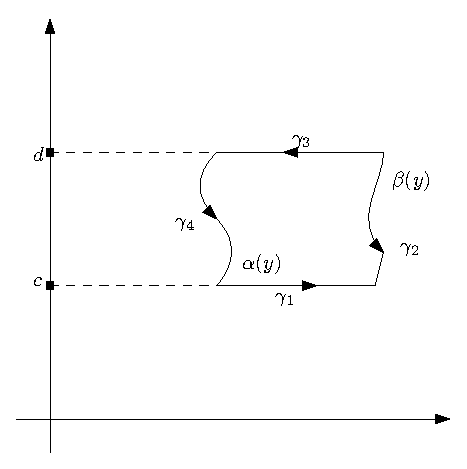
\includegraphics[width=6cm]{img/finiti/primaLeggeGreenGauss.eps}\\
		\begin{equation*}
			D:\begin{cases}
				c\leq y\leq d\\
				\alpha(y) \leq x \leq \beta (y)
			\end{cases} 
			\begin{matrix}
				\text{ e la sua frontiera è }\\ FD=\gamma_1\cup\gamma_2
			\cup \gamma_3 \cup \gamma_4
			\end{matrix}
		\end{equation*}
	\end{multicols}
	Sviluppiamo I e II membro della tesi
	\begin{description}
		\item[I membro] 
			\begin{equation*}
				\iint_{D} \frac{\partial f}{\partial x} dxdy=\int_{c}^{d}
				dy\int_{\alpha(y)}^{\beta(y)}\frac{\partial f}{\partial x} dx=
				\int_{c}^{d} f[\beta(y),y]-f[\alpha(y),y] dy
			\end{equation*}
			\begin{equation*}
				N.B.\text{ } \int_{\alpha (y)}^{\beta (y)} \frac{\partial
				f}{\partial x} dx=\left| f(x,y) \right|^{x=\beta(y)}_{x=\alpha
				(y)}=f(\beta(y),y)-f(\alpha(y), y)
			\end{equation*}
		\item[II membro]
			$F_D: \gamma_1 \cup \gamma_2 \cup \gamma_3 \cup\gamma_4$
			\begin{equation}
				\int_{+FD}f(x,y)dy=\int_{\gamma_1}f(x,y)dy+\int_{\gamma_2}f(x,y)
				dy+\int_{\gamma_3}f(x,y)dy+\int_{\gamma_4}f(x,y)dy
			\end{equation}
			\begin{multicols}{2}
				\begin{equation*}
					\begin{matrix}
						\begin{matrix}
							\gamma_1: y=c & dy=0
						\end{matrix}\\
						\gamma_2=\begin{cases}
							x=\beta(y)\\
							y\in[c,d]
						\end{cases}
					\end{matrix}
				\end{equation*}
				\begin{equation*}
					\begin{matrix}
						\begin{matrix}
							\gamma_3: y=d & dy=0
						\end{matrix}\\
						\gamma_4=\begin{cases}
							x=\alpha(y)\\
							y\in[d,c]
						\end{cases}
					\end{matrix}
				\end{equation*}
			\end{multicols}
			\begin{equation*}
				\int_{+FD}f(x,y)dy=\int_{\gamma_2}f(x,y)dy+\int_{\gamma_4}f(x,y)
				dy
			\end{equation*}
			\begin{equation*}
				\begin{matrix}
					\int_{\gamma_2}f(x,y)dy=\int_c f[\beta,y]dy &
					\int_{\gamma_4}f(x,y)dy=\int_{d}^{c}f[\alpha(y),y]dy=
					-\int_{c}^{d}f[\alpha(y),y]dy
				\end{matrix}
			\end{equation*}
			\begin{equation*}
				\int_{+FD}f(x,y)dy=\int_{c}^{d}f[\alpha(y),y]dy-
				\int_{c}^{d}f[\alpha(y),y]dy=\int_{c}^{d}f[\alpha(y),y]-
				f[\alpha(y),y]dy
			\end{equation*}
	\end{description}
	Si è così dimostrata la tesi\\
	Per cui con questa {\color{red}formula di Green-Gauss} un integrale doppio
	-- sotto opportune ipotesi -- si può trasformare in un integrale curvilineo
	esteso alla frontiera del dominio di integrazione
	\begin{equation*}
		\iint_D \frac{\partial f}{\partial x}dxdy=\int_{+F_D}f(x,y)dy
	\end{equation*}
\end{proof}
\begin{esempio}
	Calcolare $\iint_D\frac{dxdy}{\sqrt{1-x^2}}$ con $D=\begin{cases}
		xy\leq \frac{1}{4}\\
		x\geq 4\\
		0\leq x\leq \frac{\sqrt{3}}{2}
	\end{cases}$
	\begin{equation*}
		\begin{matrix}
			f(x,y)=\int\frac{1}{\sqrt{1-x^2}}dx=\arcsin x & \to \iint_D
			\frac{dxdy}{\sqrt{1-x^2}}=\int_{+F_D}\arcsin x dy & F_D=
			F_D=\gamma_1\cup \gamma_2 \cup \gamma_3
		\end{matrix}
	\end{equation*}
	\begin{figure}[ht]
		\centering
		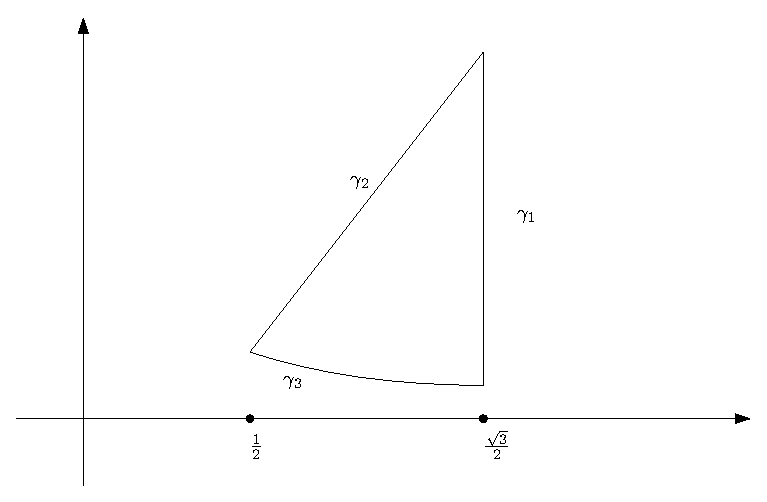
\includegraphics[width=6cm]{img/finiti/greenes.eps}
		\caption{Esempio della prima formula di Green-Gauss}
	\end{figure}
	\begin{equation*}
		\begin{matrix}
			\gamma_1: x=\frac{\sqrt{3}}{2} &
			y\in\left[\frac{\sqrt{3}}{6},\frac{1}{2}\right] & \int_{\gamma_1}\arcsin x dy=0
			& \text{ poiché } dy=0 (y=\cos t)\\
			\gamma_2: y=x & x\in \left[\frac{1}{2}, \frac{\sqrt{3}}{2}\right] &
			\text{da percorrere "al contrario"} & dy=d(x)=1dx
		\end{matrix}
	\end{equation*}
\begin{equation*}
	\begin{matrix}
		-\int_{\gamma_2} \arcsin x dy=-\int_{\frac{1}{2}}^{\frac{\sqrt{3}}{2}}
		\arcsin x dx = -\left| x\arcsin x - \int
		\frac{x}{\sqrt{1-x^2}}dx\right|_{\frac{1}{2}}^{\frac{\sqrt{3}}{2}}= 
		-\left| x\arcsin x - \int
		\sqrt{1-x^2}dx\right|_{\frac{1}{2}}^{\frac{\sqrt{3}}{2}}\\
		= -
		\left[\frac{\sqrt{3}}{2}\arcsin\frac{\sqrt{3}}{2}-\sqrt{1-\frac{3}{4}}
		- \frac{1}{2}\arcsin \frac{1}{2}-\sqrt{1-\frac{1}{4}} \right] =
		-\left[\frac{\sqrt{3}}{2}\frac{\pi}{6}+\frac{1}{2}-\frac{1}{2}
		\frac{\pi}{3} - \frac{\sqrt{3}}{2}\right]\\
	\end{matrix}
\end{equation*}
\begin{equation*}
	\begin{matrix}
		\gamma_3: &y=\frac{1}{4x}& x\in \left[\frac{1}{2},
		\frac{\sqrt{3}}{2}\right] & dy=-\frac{1}{4x} & \int_{\gamma_3}\arcsin
		xdy=\int_{\frac{1}{2}}^{\frac{\sqrt{3}}{2}}\arcsin x
		\left(\frac{1}{4x}dx\right)
	\end{matrix}
\end{equation*}
\clearpage
\begin{equation*}
	\begin{matrix}
		\int_{\gamma_3}\arcsin x
		dy=-\int_{\frac{\sqrt{3}}{6}}^{\frac{1}{2}}=y\arcsin \frac{1}{4y}dy=
		y\arcsin \frac{1}{4y}-\int
		y*\frac{1}{\sqrt{1-\frac{1}{16}}y^2}\left(-frac{1}{4y^2}\right)dy\\
		=y\arcsin\left(\frac{1}{4y}\right)-\int-\frac{1}{4y}\frac{1}{\sqrt{\frac{16
		y^2-1}{16y^2}}}dy
	\end{matrix}
\end{equation*}
	Si risolve con la sostituzione $\int\frac{1}{\sqrt{x^2-a^2}}dx$ 
\begin{align*}
	x=\sqrt{x^2-a^2}=a\tan t\\
	\sqrt{y^2-\frac{1}{16}}=\frac{1}{4}\tan t
\end{align*}
\end{esempio}
\subsubsection{Seconda formula di Green-Gauss}
\begin{teorema}
	Sia $f(x,y)$ continua in un insieme D, sia $\frac{\partial f}{\partial y}$
	continua in D, sia D un dominio normale rispetto all'asse x e sia la sua
	frontiera $F_D$ una curva regolarea tratti. Allora vale la seguente
	relazione 
	\begin{equation}
		\iint_D \frac{\partial f}{\partial y} dxdy=-\int_{+FD} f(x,y) dx
	\end{equation}
	\begin{multicols}{2}
		\subsubsection{Ipotesi}
			\begin{equation*}
				\begin{matrix}
					f(x,y)\in C^o_D\\
					\frac{\partial f}{\partial y}\in C^0_D
				\end{matrix}
			\end{equation*}
			$D$ normale rispetto all'asse $x$
			\begin{align*}
			D:\begin{cases}
				a\leq x\leq b\\
				g(x)\leq y\leq h(x)
			\end{cases}
			\end{align*}
			$F_D$ regolare a tratti
		\subsubsection{Tesi}
		\begin{equation*}
			\iint_D \frac{\partial f}{\partial y} dxdy=-\int_{+FD} f(x,y)dx
		\end{equation*}
	\end{multicols}
\end{teorema}
\begin{proof}
	Purché $f(x,y)\in C_D^o$ e $\frac{\partial f}{\partial y}\in C_D^o$, esse
	sono integrali in $D$. Il dominio $D_1$ che è normale rospetto all'esse x
	può essere descritto come
	\begin{multicols}{2}
		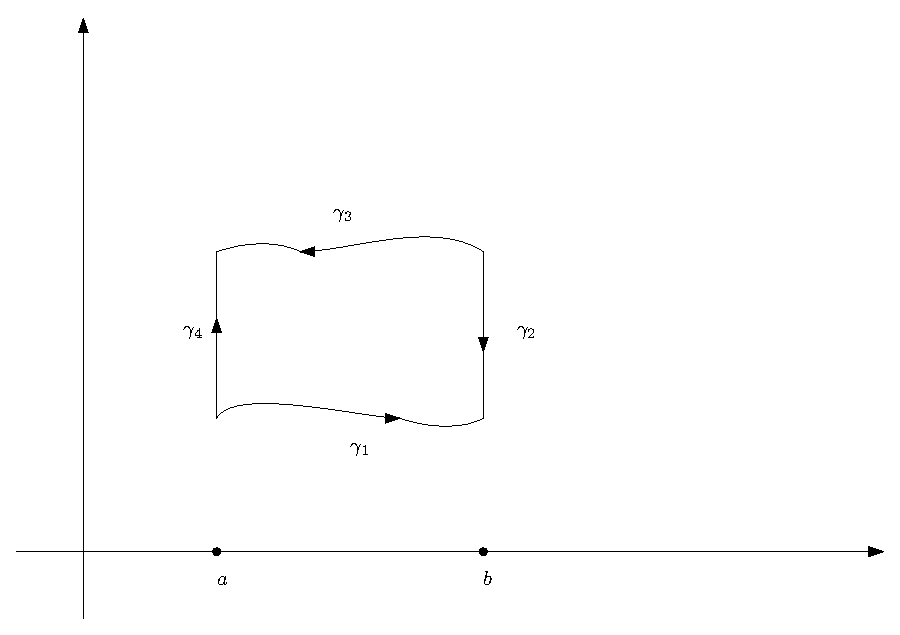
\includegraphics[width=6cm]{img/finiti/secondalegge.eps}\\
		\begin{equation*}
			D=\begin{cases}
				a\leq x\leq b\\
				g(x)\leq y\leq h(x)
			\end{cases}\begin{matrix}
				\text{ e la sua frontiera è}\\
				F_D=\gamma_1\wedge \gamma_2 \wedge \gamma_3 \wedge \gamma_4
			\end{matrix}
		\end{equation*}
	\end{multicols}
	Svuluppiamo I e II membro della tesi $\int_{h(x)}^{g(x)}\frac{\partial
	f}{\partial y} dy=|f(x,y)|^{y=h(x)}_{y=g(x)}=f[x,h(x)]-f[x,g(x)]$
	\begin{description}
		\item[I membro]
			\begin{equation*}
				\iint_D \frac{\partial f}{\partial y} dx dy=\int_{a}^{b} dx
				\int_{g(x)}^{h(x)}\frac{\partial f}{\partial y} dy=
				f[x,h(x)]-f[x,g(x)]dx
			\end{equation*}
		\item[II membro]
			\begin{equation*}
				\int_D f(x, y) dx = \int_{\gamma_1} f(x,y)dx+\int_{\gamma_2}
				f(x,y)dx+\int_{\gamma_3} f(x,y)dx+\int_{\gamma_4} f(x,y)dx
			\end{equation*}
			\begin{equation*}
				\begin{matrix}
					\gamma_2: &x=b& y\in[g(b),h(b)]dx=0\\
					\gamma_4: &x=a& y\in[g(a),b(a)]dx=0
				\end{matrix}
			\end{equation*}
			\clearpage
			\begin{equation*}
				\begin{matrix}
					\gamma_1: &y=g(x)&x\in[a,b]&\int_{\gamma_1}f(x,y) dx= 
					\int_{a}^{b}f[x,g(x)]dx\\
					\gamma_3: &y=h(x)& x\in[b, a] & \int_{\gamma_3}f(x,y)dx=-\int_{a}^{b}f[x,h(x)]dx
				\end{matrix}
			\end{equation*}
			per cui
			\begin{equation*}
				\int_{+FD}
				f(x,y)dx=\int_{a}^{b}f[x,g(x)]dx-\int_{a}^{b}f[x,h(x)]dx =
				\int_{a}^{b}f[x,g(x)]-f[x,h(x)]dx
			\end{equation*}
	\end{description}
	combiando di segno si dimostra la tesi\\
	con questa formula di {\color{red}Green-Gaun} un integrale doppio -- sotto
	opportune ipotesi -- si può trasformare in un integrale curvilineo hteso
	alla frontiera del dominio di integrazione.
	\begin{equation*}
		\iint \frac{\partial f}{\partial y}dxdy=-\int_{FD} f(x,y) dx
	\end{equation*}
\end{proof}
\subsection{Teorema della divergenza}
\begin{defi}
	Sia $\vec{F}\equiv (f(x,y),g(x,y))\in C^\prime_D$ funzione vetoriale, si
	definisce {\color{red}divergenza} di $\vec{F}$
	\begin{equation*}
		\begin{matrix}
			div \vec{F}=\frac{\partial f}{\partial x}+\frac{\partial
			f}{\partial y} & \begin{matrix}
				\text{derivata rispetto } \partial x \text{ della prima
				componente più derivata}\\
				\text{ rispetto a } \partial y \text{ della
				seconda componente}
			\end{matrix}
		\end{matrix}
	\end{equation*}
\end{defi}
\subsubsection{Teorema della divergenza \label{tdiv}}
\begin{teorema}
	Sia $\vec{F}\equiv (f(x,y), g(x,y))\in C_0^\prime$ e sia D un dominio
	normale\footnote{rispetto ad entrambi gli assi}, con la sua frontiera $F_D$
	regolare a tratti, vale la sequente relazione:
	\begin{equation*}
		\begin{matrix}
			\iint_D div \vec{F}dxdy=\int_{+FD}\vec{F}*\vec{n}ds & \text{ con }
			\vec{n} \text{ versore normale a } F_D
		\end{matrix}
	\end{equation*}
	\begin{multicols}{2}
		\subsubsection{Ipotesi:}
		\begin{equation*}
			\vec{F}\equiv (f(x,y), g(x,y))\in C_0^\prime
		\end{equation*}
		$D$ normale rispetto ad entrambi gli assi $F_D$ regolare a tratti.
		\subsubsection{Tesi:}
		\begin{equation*}
			\iint_D div \vec{F}dxdy=\int_{+FD}\vec{F}*\vec{n}ds
		\end{equation*}
	\end{multicols}
\end{teorema}
\begin{proof}
	\begin{equation*}
		\begin{matrix}
			\iint div \vec{F} dxdy=\iint_{D} \left(\frac{\partial f}{\partial
			x}\right)dxdy & \text{per definizione divergenza}
		\end{matrix}
	\end{equation*}
	Dalle ipotesi valgono le due formule di \textit{\color{red}Green-Gauss}
	\begin{equation*}
		\begin{matrix}
			\iint \frac{\partial f}{\partial x}dxdy=\int_{+FD}f(x,y)dy &:&
			\iint_D \frac{\partial f}{\partial y}dxdy=-\int_{+FD}g(x,y)dx
		\end{matrix}
	\end{equation*}
	Devo così dimostrare che $f(x,y)dx-g(x,y)dy=\vec{F}*\vec{n}ds$\\
	Ricavo il versore normale $\vec{n}$: $F_D$ regolare a tratti ed è quindi ed
	è quindi esprimibile come unione di curve regolari di espressione
	parametrica
	\begin{equation*}
		\begin{matrix}
			\begin{cases}
				x=x(t)\\
				y=y(t)
			\end{cases} t\in [a,b] & \exists x^\prime(t).y^\prime(t)\text{ perché la
			curva è regolare.}

		\end{matrix}
	\end{equation*}
	Il vettore tangente $\vec{t}=(x^\prime(t),y^\prime(t))$, scambiando le
	componenti e cambiandone una di segno si ottine il vettore normale
	$(y^\prime(t),-x^\prime (t))$; dividendo per la norma
	$\sqrt{[x^\prime(t)]^2+[y^\prime(t)]^2}$ si ha il versore normale $\vec{n}$
	\begin{equation*}
		\vec{n}\equiv
		\left(\frac{y^\prime(t)}{\sqrt{[x^\prime(t)]^2+[y^\prime(t)]^2}}:
		\frac{x^\prime (t)}{\sqrt{[x^\prime(t)]^2+[y^\prime(t)]^2}}\right)
	\end{equation*}
	Svolgo ora il prodotto scalere $\vec{F}*\vec{n}ds$, ricordando che
	$ds=\sqrt{[x^\prime(t)]^2+[y^\prime(t)]^2}$ 
	\begin{align*}
		\vec{F}\equiv (f(x,y), g(x,y))\\
		\vec{F}*\vec{n}ds=\left(\frac{f(x,y)y^\prime(t)}{\sqrt{[x^\prime(t)]^2+[y^\prime(t)]^2}}-\frac{g(x,y)x^\prime(t)}{\sqrt{[x^\prime(t)]^2+[y^\prime(t)]^2}}\right)\sqrt{[x^\prime(t)]^2+[y^\prime(t)]^2}
	\end{align*}
	\begin{equation*}
		\begin{matrix}
			\begin{matrix}
				x^\prime(t)=dx\\
				y^\prime(t)=dy
			\end{matrix}&\vec{F}*\vec{n}ds=f(x,y)dy-g(g,y)dx
		\end{matrix}
	\end{equation*}
	Quindi 
	\begin{eqnarray*}
		\iint_D div \vec{F}dxdy=\int_{+FD}f(x,y)dy-g(x,y)dx & div
		\vec{F}=\frac{\partial f}{\partial x}+ \frac{\partial g}{\partial y}
	\end{eqnarray*}
	Il teorema della divergenza (\ref{tdiv}) vale anche in $R^3$, in forma
	vettoriale
	\begin{eqnarray*}
		\iiint_{V}div \vec{F} dxdydz = \iint_{+\Sigma}\vec{F}*\vec{n}ds &\vec{F}
		=\frac{\partial f}{\partial x}+ \frac{\partial g}{\partial y} + 
		\frac{\partial h}{\partial z}
	\end{eqnarray*}
\end{proof}
\begin{esempio}
	calcolare utilizzando il teorema della divergenza $\iint_D div\vec{F}dxdy$
	con $\vec{F}\equiv (-2x^3y;\frac{1}{2}xy), D=\{x^2+y^2\leq 1\}$
	\begin{equation*}
		div \vec{F}=-\frac{2x^3y}{\partial x}+\frac{-\frac{1}{2}xy}{\partial
		y}= -6x^2y-\frac{1}{2}x
	\end{equation*}
	\begin{equation*}
		\iint_D(-6x^2y-\frac{1}{2}x)dxdy=\int_{+FD}f(x,y)dy+g(x,y)dx=\int_{+FD}
		-2x^2ydy+\frac{1}{2}xydx
	\end{equation*}
	\begin{eqnarray*}
		FD:x^2+y^2=1 & \begin{cases}
			x=\cos t \\
			y=\sin t
		\end{cases} t\in [0,2\pi] & \begin{matrix}
			dx=-\sin t dt\\
			dy=\cos t dt
		\end{matrix}
	\end{eqnarray*}
	\begin{eqnarray*}
		\int_{0}^{2\pi} -2\cos^3 t \sin t\cos t dt + \frac{1}{2}\cos t \sin t
		(-\sin t) dt= +\int_{0}^{2\pi} \left(-2\cos^4t\sin t +
		\frac{1}{2}\sin^2t \cos t\right)\\=\begin{vmatrix}
			-\frac{2}{5} \cos^5 t - \frac{7}{6}\sin^3 t
		\end{vmatrix}^{2\pi}_0 =-\frac{2}{5}-0+\frac{2}{5} -0=0
	\end{eqnarray*}
\end{esempio}
\subsubsection{Applicazioni della formula di Green-Gauss}
Rimandi teorici a partire da (\ref{fGreen-Gauss}) -- Calcolo dell'area di
dominio piani\\
Ricordando le formule di \texttt{Green-Gauss} $\iint_D \frac{\partial
f}{\partial x}dxdy=\int_{+FD} f(x,y)dy:\iint_D \frac{\partial f}{\partial
y}dxdy =-\int_{+FD}f(x,y)dx$ nella formula dell'area $\frac{\partial
f}{\partial x}=1$ o $\frac{\partial f}{\partial y}=1$ per cui $f(x,y)=x$ o
$f(x,y)=y$\\
Si ha così $A=\iint_D dxdy=\int_{+FD}xdy=-\int_{+FD}ydx\to
\int_{+FD}xdy-\int_{+FD}ydx=2\iint_Ddxdy$ si ha:
\begin{equation*}
	\boxed{A=\frac{1}{2}\int_{+FD}xdy-ydx}
\end{equation*}
\clearpage
\begin{esempio}
	Calcolare l'area del dominio delimitato dall'ellisse con semiassi a e b
	\begin{eqnarray*}
		F_D:\begin{matrix}
			x=a\cos t \\
			y=b\sin t
		\end{matrix}& t\in [0,2\pi]&\begin{matrix}
			dx=a\sin t \\
			dy=b\cos t
		\end{matrix}
	\end{eqnarray*}
	\begin{eqnarray*}
		\iint dxdy= \frac{1}{2}\int_{+FD}xdy-ydx=\frac{1}{2}\int_{0}^{2\pi}a
		\cos t (b\cos t)- b\sin t (-a \sin
		t)dt\\=\frac{1}{2}\int_{0}^{2\pi}ab\cos^2t+ab\cos^2 t +
		ab\sin^2t=\frac{1}{2}ab\int_{0}^{2\pi}dt=ab\pi
	\end{eqnarray*}
\end{esempio}

\section{Forma differenziali Lineari}
Si definisce differenziale lineare $\omega$
\begin{align*}
	\mathds{R}^2\Rightarrow \omega=f(x,y)dx+g(x,y)dy\\
	\mathds{R}^3\Rightarrow \omega= F_1(x,y,z)dx+F_2(x,y,z)dy+F_3(x,y,z)dz
\end{align*}
\subsection{Integrazione delle forme differenziali}
\begin{defi}
	Sia $\omega$ una forma differenziale continua in un insieme
	$D$\footnote{ivi integrabile} e sia $\gamma$ una curva regolare a tratti
	contenuta in D, di equazioni parametriche $\gamma \equiv (x(t),y(t), z(t)),
	t\in [a,b]$. Si definisce {\color{red}integrale della forma differenziale
	esteso alla curva $\gamma$}
	\begin{eqnarray*}
		\int_{\gamma} \omega ds=\int_{\gamma}
		F_1(x,y,z)dx+F_2(x,y,z)dy+F_3(x,y,z)dz=\int_{a}^{b}
		F_1(x(t),y(t),z(t))x^\prime (t)\\
		+F_2(x(t),y(t),z(t))y^\prime (t) + F_3(x(t),y(t),z(t))z^\prime (t)dt
	\end{eqnarray*}
	L'integrale rettilineo che va tra gli estremi su cui è preso t\\
	La funzione $F\equiv[F_1(x,y,z),F_2(x,y,z),F_3(x,y,z)]$ viene calcolata
	sui punti della curva $\gamma$\footnote{funzione composita}
	\begin{equation*}
		\text{I differenziali sono } \begin{cases}
			dx=x^\prime(t)\\
			dy=y^\prime(t)\\
			dz=z^\prime(t)
		\end{cases}
	\end{equation*}
\end{defi}
Le {\color{red} proprietà delle forme differenziali lineari} derivano dalle
proprietà degli integrali curvilinei
\begin{itemize}
	\item Linearità:
		\begin{eqnarray*}
			\int_{\gamma}\omega_1 +\omega_2 ds=\int_\gamma \omega_1ds
			+\int_\gamma \omega_2 ds\\
			\alpha\int_\gamma \omega ds=\int_\gamma \alpha \omega ds 
		\end{eqnarray*}
	\item Additività:
		\begin{eqnarray*}
			\gamma=\gamma_1\wedge \gamma_2\wedge \dots \wedge \gamma_n &
			\int_\gamma \omega ds =\int_{\gamma_1} \omega ds + \int_{\gamma_2}
			\omega ds + \dots +\int_{\gamma_n} \omega ds
		\end{eqnarray*}
\end{itemize}
\subsection{Forme differenziali esatte}
\begin{defi}
	Sia $\omega$ una forma differenziabile, essa si dice {\color{red}esatta},
	se esiste una funzione $f(x,y,z)$\footnote{detta \color{red}funzione
	potenziale} tale che il suo differenziale primo sia $\omega$
	\begin{equation*}
		\omega=F_1(x,y,z)dx+F_2(x,y,z)dy+F_3(x,y,z)dz\text{ è esatto
		se }\exists f(x,y,z):df=\omega
	\end{equation*}
	poiché $df=fx(x-x_0)+fy(y-y_0)+fz(z-z_0)$
	\begin{equation*}
		\text{se $\omega$ è esatta }\begin{cases}
			F_1(x,y,z)=\frac{\partial f}{\partial x}\\
			F_2(x,y,z)=\frac{\partial f}{\partial y}\\
			F_3(x,y,z)=\frac{\partial f}{\partial z}
		\end{cases}
	\end{equation*}
\end{defi}
\subsection{Forma differeniali chiusa}
In $R^2$: consideriamo una forma differenziale $\omega$ in $R^2$ esatta
\begin{equation*}
	\omega=F_1(x,y)dx+F_2(x,y)dy
\end{equation*}
Per definizione di forma differenziale esatta
\begin{eqnarray*}
	\exists f(x,y):df=\omega& \text{cioè } F_1(x,y)=\frac{\partial f}{\partial
	x} & F_2(x,y)=\frac{\partial f}{\partial y}
\end{eqnarray*}
Con $f(x,y)\in C^2$ derivo F, rispetto a $y$ e $F_2$ rispetto $\partial x$ -- 
Così vale il teorema di Schwarz (\ref{Schwarz})
\begin{eqnarray*}
	\frac{\partial}{\partial y}F_1(x,y)=\frac{\partial}{\partial
	y}\left(\frac{\partial f}{\partial x}\right) =f_{xy} &\frac{\partial
	F_2}{\partial x}=\frac{\partial}{\partial x} \left(\frac{\partial
	f}{\partial y}\right)=f_{yx}
\end{eqnarray*}
$f_{xy}=f_{yx}\to \frac{\partial F_1}{\partial y}=\frac{\partial F_2}{\partial
x}$ \\
Se è vera tale relazione, la forma differenziale si dice {\color{red}chiusa}.
\begin{center}
	\fbox
	{
		\begin{minipage}{0.85\textwidth}
			In $R^3$: Definiamo primo il rotore di una funzione vettoriale di 
			classe $C^\prime$ \\
			Sia $F\equiv (F_1(x,y,z),F_2(x,y,z),F_3(x,y,z))$. Il rotore di F è 
			il determinante:
			\begin{equation*}
				rot \vec{F}=\begin{vmatrix}
					\vec{l} &\vec{j} &\vec{k} \\
					\partial x & \partial y & \partial z\\
					F_1 & F_2 & F_3
				\end{vmatrix}=\left(\frac{\partial F_3}{\partial y}-
			\frac{\partial F_2}{\partial z}\right)\vec{l} -
				\left(\frac{\partial F_3}{\partial x}-
			\frac{\partial F_1}{\partial z}\right)\vec{j} +
				\left(\frac{\partial F_1}{\partial z}-
				\frac{\partial F_2}{\partial x}\right)\vec{k}
			\end{equation*}
			Consideriamo ora una forma differenziale lineare $\omega$ in $R^3$
			\begin{eqnarray*}
				\omega =F_1(x,y,s)dx+F_2(x,y,z)dy+F_3(x,y,z)dz\\
				\text{con } F\equiv(F_1(x,y,z),F_2(x,y,z), F_3(x,y,z))
			\end{eqnarray*}
			$\omega$ è chiusa se $rot F=0$
			\begin{equation*}
				rot\vec{F}=\left(\frac{\partial F_3}{\partial y}-
			\frac{\partial F_2}{\partial z}\right)\vec{l} -
				\left(\frac{\partial F_3}{\partial x}-
			\frac{\partial F_1}{\partial z}\right)\vec{j} +
				\left(\frac{\partial F_1}{\partial z}-
				\frac{\partial F_2}{\partial x}\right)\vec{k}
			\end{equation*}
			$rot \vec{F}$ è un vettore, è nullo quando tutte le sue componenti
			sono nulle.
			\begin{equation*}
				\begin{matrix}
				\frac{\partial F_3}{\partial y}=\frac{\partial F_2}{\partial z}
				& ; & \frac{\partial F_3}{\partial x}=\frac{\partial
				F_1}{\partial z} & ; &\frac{\partial F_1}{\partial z}=
				\frac{\partial F_2}{\partial x}
				\end{matrix}
			\end{equation*}
		\end{minipage}
	}
\end{center}
\clearpage
\subsection{Condizioni necessarie affinché una forma differenziale sia esatta}
Se $\omega$ è esatta allora è chiusa
\paragraph{Condizione necessaria:} Affinché $\omega$ sia esatta è che deve
essere chiusa\\
cioè se $\omega$ non è chiusa \texttt{può} essere esatta,
invece, se $\omega$ non è chiusa \underline{sicuramente \color{red} non} è esatta
\begin{multicols}{2}
	\begin{equation*}
		R^2\text{ }\frac{\partial F_1}{\partial x}=\frac{\partial F_2}{\partial y}
	\end{equation*}
	\begin{equation*}
		R^2\text{ } rot \vec{F}=0
	\end{equation*}
\end{multicols}
\begin{proof}
	Per definizione $rot F=\begin{vmatrix}
		l & j & k \\
		\alpha_x & \alpha_y & \alpha_z\\
		F_1 & F_2 & F_3
	\end{vmatrix}$\\
	Se $\omega$ è esatta\\
	esiste la funzione potenziale $f(x,y,z)$ tale che $df=\omega$, per cui
	$F_1=\frac{\partial f}{\partial x};F_2=\frac{\partial f}{\partial y};
	F_3=\frac{\partial f}{\partial z}$ da cui
	\begin{equation*}
		rot F=\begin{vmatrix}
			l & j & k\\
			\partial_x &\partial_y & \partial_z \\
			\frac{\partial f}{\partial x} &\frac{\partial f}{\partial
			y} & \frac{\partial f}{\partial z}
		\end{vmatrix}=(f_{zy}-f_{yz})\vec{l} - (f_{zx}-f_{xz})\vec{j}+
		(f_{yx}-f_{xy})\vec{k}
	\end{equation*}
	Se $f(x,y,z)\in C^2$ vale il teorema di Schwarz (\ref{Schwarz}), così tutte
	le componenti di $rot F$ sono nulle $rot F = 0$
\end{proof}
\subsubsection{Proprietà delle forme differenziale lineari esatte}
\begin{description}
	\item[Teorema 1 -] L'integrale curvilineo di una forma differenziale
		lineare esatta non dipende dalla curva (percorso) ma solo dagli
		estremi\\
		Sia $omega$ esatta in un insieme $V$ e sia $\gamma \subset V$ un arco di
		curva regolare di estremi $P_0$ e $P_1$ allora $\displaystyle\int_\gamma
		F_1(x,y,z)dx + F_2(x,y,z) dy+ F_3(x,y,z)dz=f(P_1)-f(P_0)$
		\begin{multicols}{2}
			\subsubsection{Ipotesi:}
			$\omega$ esatta in $V$
			\begin{eqnarray*}
				\gamma=\begin{cases}
					x=x(t) \\
					y=y(t)\\
					z=z(t)
				\end{cases} & t\in[a,b] &\text{regolare}\\
				\gamma \subset V
			\end{eqnarray*}
			\subsubsection{Tesi:}
				$\displaystyle\int_\gamma
				F_1dx + F_2 dy+ F_3=f(P_1)-f(P_0)$
		\end{multicols}
		\begin{proof}
			Per definizione di integrale curvilineo
			\begin{eqnarray*}
				\int_\gamma F_1(x,y,z)dx + F_2(x,y,z) dy+ F_3(x,y,z)dz =
				\int_{a}^{b} [F_1(x(t),y(t),z(t)) + F_2(x(t),y(t),z(t))\\ +
				F_3(x(t),y(t),z(t))]dt
			\end{eqnarray*}
			per ipotesi $\omega$ è esatta, per cui esiste una funzione
			potenziale tale che $df=\omega$ da cui si ha:
			\begin{equation*}
				\begin{matrix}
					F_1(x(t),y(t),z(t))=\frac{\partial f}{\partial x}(x(t),y(t),z(t)) \\
					F_2(x(t),y(t),z(t))=\frac{\partial f}{\partial y}(x(t),y(t),z(t)) \\
					F_3(x(t),y(t),z(t))=\frac{\partial f}{\partial z}(x(t),y(t),z(t))
				\end{matrix}
			\end{equation*}
			L'integrale diventa $\int_{a}^{b} [F_1(x(t),y(t),z(t)) + 
			F_2(x(t),y(t),z(t)) + F_3(x(t),y(t),z(t))]dt$
			\clearpage
			Per il teorema della derivata della funzione composta,
			l'espressione da integralre è
			$\frac{\partial f}{\partial t}(x(t),y(t),z(t))$ per cui
			$\int_{a}^{b}\frac{\partial f}{\partial t}(x(t),y(t),z(t))dt=
			\begin{vmatrix}
				f(x(t),y(t),z(t))
			\end{vmatrix}^d_a=f(P_1)-f(P_0)$ con $\begin{matrix}
				P_0(x(a),y(a),z(a))\\
				P_1(x(b),y(b),z(b))
			\end{matrix}$
		\end{proof}
	\item[Teorema 2 -] Sia $\omega$ una forma differenziale lineare continua in
		un insieme $A$ aperto connsso.\\
		Le sequanti affermazioni sono vere:
		\begin{tasks}
			\task $\omega$ è esatta in A
			\task per $\forall \gamma \subset A$ chiusa $\int_\gamma \omega=0$
			\task se $\gamma_1$ e $\gamma_2$ hanno gli stessi estremi e lo
			stesso verso di percorrenta si ha
			\begin{equation*}
				\int_{\gamma_1} \omega=\int_{\gamma_2}\omega
			\end{equation*}
		\end{tasks}
\end{description}
\section{Funzione potenziale}
\begin{defi}
	Se $\omega$ è esatta, esiste una funzione $f(x,y)$, detta
	{\color{red}funzione potenziale}, tale che il suo differenziale eguaglia
	$\omega$
	\begin{equation*}
		df=\omega
	\end{equation*}
	f(x,y) è definita a meno di una costante, infatti $df(x,y)= d(f(x,y)+k)$
	con $\omega$ esatta, la funzione potenziale si triva con 
	\begin{equation*}
		f(x,y)=\int_\gamma \omega=\int_\gamma F_1(x,y)dx+F_2(x,y)dy
	\end{equation*}
	Poiché $\omega$ è esatta, quest'integrale curvilineo non dipende dal
	pecorso, ma sdamente dagli estremi. \\
	Per cui considero un percorso semplice su cui integrare i segmenti
	paralleli agli assi
	\begin{multicols}{2}
          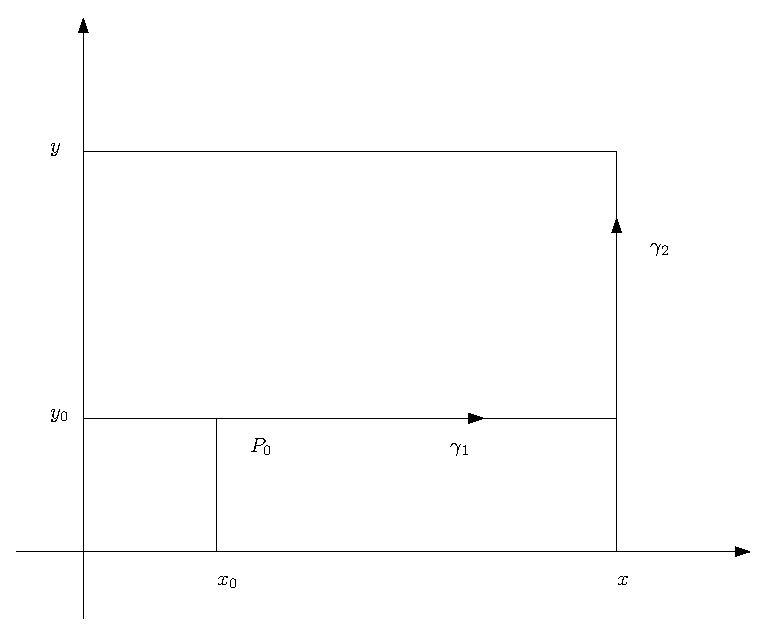
\includegraphics[width=6cm]{img/finiti/es-fun-pot.eps}\\
          \begin{eqnarray*}
            \begin{matrix}
              \gamma=\gamma_1+\gamma_2 & \gamma_1 dy=0\\
              			       & \gamma_2 dx=0
            \end{matrix}
          \end{eqnarray*} 
	\end{multicols}
        \begin{eqnarray*}
          f(x,y) = \int_\gamma F_1dx+F_2 dy= \int_{\gamma_1} F_1(x,y)dx+F_2 (x,y)dy+
          \int_{\gamma_2} F_1(x,y)dx+F_2(x,y)dx\\
          =\int_{x_0}^{x}F_1(t,y_0)dt+F_2(t,y_0)dy+\int_{y_0}^yF_1(x_0,m)dx+F_2(x_0,m)dm
          =\int_{x_0}^{x}F_1(t,y_0)dt+\int_{y_0}^yF_2(x_0,m)dm
        \end{eqnarray*}        
\end{defi}
\clearpage
\subsection{Condizioni sufficiente affinché una forma differenziale lineare sia Esatta}
\begin{defi}
  Sia $\omega$ una differenziale chiusa in un insieme A semplicemente connesso.
  Allora $\omega$ è esatta in A.
  \begin{multicols}{2}
    \subsubsection{Ipotesi:}
    $\omega$ è chiusa in A\\
    A semplicemente connesso
    \subsubsection{Tesi:}
    $\omega$ è esatta in A
  \end{multicols}
  Prendo una qualunque curva $\gamma$ chiusa in A, poiché A è semplicemente connesso,
  ogni $\gamma$ è frontiera di un sottoinsieme $A^\prime$ di A.\\
  Per cui $\int_\gamma \omega =\int_{+FA^\prime}F_1(x,y)dx+F_2(x,y)dy$ --
  Per il teorema della divergenza (\ref{fGreen-Gauss})
  \begin{equation*}
    \int_{+FA^\prime}F_1(x,y)dx+F_2(x,y)dy=\iint_{A^\prime}-
    \frac{\partial F_1(x,y)}{\partial y} dxdy+
    \iint_A\frac{\partial F_2(x,y)}{\partial x} dxdy
  \end{equation*}
  Per ipotesi $\omega$ è chiusa cioè $\frac{\partial F_1(x,y)}{\partial y}=
  \frac{\partial F_2}{\partial x}(x,y)$\\
  Per cui si ha:
  \begin{equation*}
    \iint_{A^\prime}-
    \frac{\partial F_1(x,y)}{\partial y} dxdy+
    \iint_A\frac{\partial F_2(x,y)}{\partial y} dxdy=0
  \end{equation*}
  ovvero $\int_\gamma \omega =0$ l'integrale per stato calcolato segliendo una qualunque
  $\gamma$ chiusa in A. Tale il risultato è una caratteristica delle forme differenziali
  lineari esatte, per cui si può concludere che $\omega$ è esatta in A.
\end{defi}
\subsection{Condizione necessaria e sufficiente}
Il teorema precedente è condizione necessaria e sufficiente affinché una forma differenziale lineare $\omega$ si esatta.
\begin{eqnarray*}
  \omega \text{ è esatta in A} \Leftrightarrow \omega \text{ è chiuse in } A\\
  \omega \text{ esatta in A} \Rightarrow \omega \text{ chiusa in } A\\
  \omega \text{ chiusa in A} \Rightarrow \omega \text{ esatta in } A
\end{eqnarray*}
\subsection{Teorema di Stokes (o del rotore)\label{stokes}}
Con il teorema di Stoches -- sotto opportune condizione --  è possibile trasformare un
integrale superficiale in un integrale curvilineo, esteso al bordo della superfice.\\
Sia $F(x,y,z)\equiv (F_1(x,y,z),F_2(x,y,z),F_3(x,y,z))$ un campo\footnote{o funzione}
vettoriale definito in un insieme $V\subset R^3$, sia $F(x,y,z)\in C_V^\prime$\\
Sia $\Sigma$ una porzione di superficie $\subset V$, $\Sigma$ regolare, orientabile,
dotata di bordo orientabile che sia una curva regolare o regolare a tratti.
\begin{eqnarray*}
  \Sigma: \vec{r}=r(u,v)=\begin{cases}
                           x=x(u,v)\\
                           y=y(u,v)\\
                           z=z(u,v)
                         \end{cases} & (u,v)\in D & \vec{r}(u,v)\in C_D^2
\end{eqnarray*}
Allora vale la seguente uguaglianza
\begin{equation*}
  \iint_\Sigma rot \vec{F}*\vec{n}_e d\sigma=\int_{+B\Sigma}\vec{F}*\vec{t}ds
\end{equation*}
dove $rot \vec{F}=\begin{vmatrix}
                    \vec{l} & \vec{j} & \vec{k} \\
                    \partial x & \partial y & \partial z\\
                    F_1 & F_2 & F_3
                  \end{vmatrix}\vec{n}_e$ versore noramle alla superficie $\Sigma$
                  $n_e\frac{\vec{r}_u\wedge \vec{r}_v}{||\vec{r}_u \wedge \vec{r}_v||}$
                  $dr$ elemento differenziale d'area $M=\begin{pmatrix}
                                                          x_u & y_u & z_u \\
                                                          x_v & y_v & z_v
                                                        \end{pmatrix}$
                                                        $dr=\sqrt{j_1^2+j_2^2+j_3^2}$
\begin{eqnarray*}
  J_1=\begin{vmatrix}
        y_u &z_u\\
        y_v &z_v
      \end{vmatrix}
  & J_2=\begin{vmatrix}
        x_u &z_u\\
        x_v &z_v
        \end{vmatrix}
  & J_3=\begin{vmatrix}
        x_u &z_u\\
        x_v &z_v
      \end{vmatrix}
\end{eqnarray*}
$B\Sigma$ bprdp della superficie $\begin{cases}
                                    x=x(t)\\
                                    y=y(t)\\
                                    z=z(t)
                                  \end{cases}$\\
$\vec{t}$ versore tangente al bordo -- $ds$ coerento differenziale di lunghezza $ds=\sqrt{[x^\prime(t)]^2+[y^\prime(t)]^2+[z^\prime(t)]^2}$
\paragraph{In forma cartesiana} La superficie $\omega$ è $\{z=f(x,y), (x,y)\in D\}, f(x,y)\in C^2$ -- la direzione normale $n_e\equiv \left(\frac{-fx}{\sqrt{1+f_x^2+f_y^2}};
  \frac{-fy}{\sqrt{1+f_x^2+f_y^2}}; \frac{1}{\sqrt{1+f_x^2+f_y^2}}\right)$ 
\begin{eqnarray*}
  ds=\sqrt{1+f_x^2+f_y^2}\\
  rot \vec{F}=\begin{vmatrix}
                \vec{l} & \vec{j} & \vec{k} \\
                \partial x & \partial y & \partial z \\
                F_1 & F_2 & F_3
              \end{vmatrix} = A \vec{l} + B\vec{j} + C\vec{k}\\
  \iint_\Sigma rot F_0 n_e dv=\int_{+B\Sigma} F_0 tds\\
  \iint_A\frac{-Afx-Bfy+X}{\sqrt{1+f_x^2+f_y^2}}*\sqrt{1+f_x^2+f_y^2}=\int_{+B\Sigma}
  \underbrace{F_1dx+F_2dy+F_3}_\omega dz
\end{eqnarray*}
Il prodotto scalare $\vec{F}*n_e$ è detto {\color{red}flusso}\\
$\iint_\Sigma rot F_0 n_e dv$ Integrale del flusso del rotore attraverso la superficie
$\Sigma$
\begin{description}
\item[Corollario 1]
  \begin{defi}
    Sia $n(x,y,z)\in C_V^2,V\subset R^3$, sotto le ipotesi di validità di Stokes
    (\ref{stokes})
    \begin{equation*}
      \int_{+B\Sigma}\nabla n * tds =0
    \end{equation*}
    Infatti per il teorema di Stokes $\int_{+B\Sigma}\nabla h*t ds=\iint_\Sigma rot \nabla h*n_e dv$
    \begin{eqnarray*}
      \nabla h=(hx,hy,hz)\\
      rot \nabla h=\begin{vmatrix}
                     \vec{l} & \vec{j} &\vec{k}\\
                     \partial x & \partial y & \partial z\\
                     hx & hy & hz
                   \end{vmatrix}
      =(h_{yx}-h_{xy})\vec{l}- (h_{zx}-h_{xz})\vec{j} + (h_{yx}-h_{xy})\vec{k}\\
      rot \nabla h=0\\
      \text{Da cui } \int_{+B\Sigma}\nabla h * t ds=0
    \end{eqnarray*}
  \end{defi}
  \clearpage
\item[Corollario 2]
  \begin{defi}
    Sotto le validità del teorema di Stokes (\ref{stokes}), date due superfici $\Sigma_1$
    e $\Sigma_2$ di egual bordo. Si ha
    \begin{equation*}
      \iint_{\Sigma_1} rot F_0 n_e dr_1=\iint_{\Sigma_2}F_0n_e dr_2
    \end{equation*}
   Infatti per il teorema di Stokes
  \begin{multicols}{2}
    \paragraph{I membro}
    \begin{equation*}
      \int_{+B\Sigma_1}F_0tds
    \end{equation*}
    \paragraph{II membro}
    \begin{equation*}
      \int_{+B\Sigma_2}F_0t ds
    \end{equation*}
  \end{multicols}
  poiché $B\Sigma_1=B\Sigma_2$ per ipotesi, i due integrali sono uguali. Quindi il flusso
  del rotore non dipende dalla superficie ma dal bordo.
  \end{defi}
\end{description}


\chapter{Successioni e serie}
\section{Successioni di costanti}
\begin{defi}
  Si definisce successione $a_n$ una funzione in N (numeri naturali) e codominio in R.\\
  È possibile rappresentare una successione sul pieno cartesiano, con l'asse delle
  ascisse N e quello delle ordinate R.
\end{defi}

\section{Limite di successioni}
\subsection{Limite finito di una successione}
\begin{defi}
  Si definisce limite finito della succesione $a_n$ ($a_n$ converge) il numero reale
  $\gamma$ tale che:
  \begin{eqnarray*}
    \lim_{n\to \infty} a_n=\gamma & \forall \xi >0, \exists P_\xi \in N:\forall n > P_\xi\\
                                  & \abs{a_n-\gamma} < \xi
  \end{eqnarray*}
  Una successione che per $n\to \infty$ ha limite finito si dice {\color{red}convergente}
\end{defi}
\subsubsection{Limite infinito di una successione}
$bn\to +\infty$ se
\begin{eqnarray*}
  \lim_{n\to\infty}bn=+\infty & \forall M>0, \exists P_M:\forall n > P_m & b_R>M
\end{eqnarray*}
Una successione che per $n\to \infty$ ha infinito si dice {\color{red}divergente} --
Se una successione nè converge, nè diverge, diciamo che è {\color{red}irregolare} o
{\color{red}indeterminata}, cioè non esiste $\lim\limits_{n\to\infty}$.
\section{Successioni Limitatre, illimitate, crescenti e decrescenti}
Limitata superiormente
\begin{eqnarray*}
  a_n \text{ è {\color{red} limitata superiormente} se } & \exists k:\forall n \in N
  & a_n\leq k\\
  a_n \text{ è {\color{red} limitata inferiormente} se} & \exists h: \forall n\in N
  & a_n \geq h\\
  a_n \text{ è {\color{red} limitata} se} & \text{è limita inferiormente e superiormente}
  & h\leq a_n\leq k\\
  a_n \text{ è {\color{red}monotona crescente} se} & \forall n: & a_n < a_{n+1}\\
  a_n \text{ è {\color{red}monotona decrescente} se} & \forall n: & a_n > a_{n+1}
\end{eqnarray*}
\clearpage
\subsection{Operazioni algebriche e teoremi sui limiti di successioni}
\begin{defi}
	Poiché le successioni sono una particolare classe di funzioni si estendono
	le gegole dell'algebra dei limiti e i teoremi studiati per le funzioni.
	nel calcolo di un limite, si può sostituire la successione con la funzione
	ad essa associata e calcolare il limite. Alle successioni {\color{red}NON}
	si può applicare il teorema di De l'Hospital perché le successioni non
	hanno derivate. Nel calcolo di un limite si può sostituire la successione
	con la funzione ad essa associata e si può applicare il teorema di
	del'hospital alla funzione (non alla successione)
\end{defi}
\subsection{Serie numeriche}
Una {\color{red}aria} è una somma di infiniti numeri reali. Sia ($a_n$) una
successione $a_n=(a_1,a_2, \dots,a_n)$. Definiamo {\color{red}serie
$\displaystyle\sum_{\infty}^{n=1}a_n=a_1+a_2+\dots+a_n$}\\
Sia ($S_n$) la successione delle somme parziali così definite
\begin{equation*}
	S_n=(S_1,S_2,S_3,\dots,S_n,S_{n+1},\dots)
\end{equation*}
\begin{eqnarray*}
	\begin{matrix}
		S_1=a_1\\
		S_2=a_1+a_2\\
		S_3=a_1+a_2+a_3
	\end{matrix} &\text{ se }\lim\limits_{n\to\infty}S_n=\begin{cases}
		S\in R\text{ (rinito)} & \text{\color{red}convergente}\\
		\pm \infty & \text{\color{red}divergente}\\
		\nexists &\text{\color{red}indeterminata}
	\end{cases}
\end{eqnarray*}
\subsection{Cordizione necessaria affinché una serie converga}
Sia $\displaystyle\sum_{n=1}^{\infty}a_n$ una serie convergente, allora
$\lim\limits_{n\to\infty}a_n=0$
\subsubsection{Condizione necessaria e sufficiente affinché esista il limite --
criterio di Cauchy}
\begin{eqnarray*}
	\lim_{n\to \infty} a_n=a_0 &\Leftrightarrow & \forall \xi >0 \exists v_\xi
	: \forall p_1q>v_\xi, p_1q\leftarrow N \\
	&& \abs{a_p-a_q}<\xi
\end{eqnarray*}
Esiste il limite della successione $a_n$ se e solo se per ogni $\xi >0$ esiste
un indice\footnote{che dipende da $\xi$} tale che, presi due qualunque numeri
naturali $p$ e $q$ maggiori di quell'indice la distanza tra gli elementi $a_p$
e $a_q$
\section{Particolari tipi di serie}
\subsubsection{Serie telescopica}
$\displaystyle\sum_{n=1}^{\infty}a_n-a_{n+1}$ Differenza tra due termini
successivi
\subsubsection{Serie armonica}
$\displaystyle\sum_{n=1}^{\infty}\frac{1}{n^\alpha}$ al variare di 
$\alpha \in R$, la serie ha caratteri diversi $\begin{cases}
	\text{Converge} & a\leq 2, \alpha=0\\
	\text{Diverge} &\alpha \leq 1\\
	\not{} &1\leq \alpha \leq 2
\end{cases}$
\subsubsection{Serie geometriche}
$\displaystyle\sum_{n=1}^{\infty}q^n$ il rapporto tra un termine e il
precedente è costante.

\subsection{Assoluta e semplice convergenza}
Serie a segno positivo
\begin{equation*}
	\begin{matrix}
		\displaystyle\sum_{n=1}^{\infty} a_n& \begin{matrix}
			\text{si definisce a termini di segno positivo se } \forall n>
			\bar{n} &a_n>0\\
			\text{finiti Termini negativi, infiniti termini positivi}
		\end{matrix}
	\end{matrix}
\end{equation*}
Serie a segno negativo
\begin{equation*}
	\begin{matrix}
		\displaystyle\sum_{n=1}^{\infty} b_n& \begin{matrix}
			\text{si definisce a termini di segno positivo se } \forall n>
			\bar{n} &b_n<0\\
			\text{finiti Termini positivi, infiniti termini negativi}
		\end{matrix}
	\end{matrix}
\end{equation*}
Sia a segno qualunque
\begin{equation*}
	\begin{matrix}
		\displaystyle\sum_{n=1}^{\infty} c_n& \begin{matrix}
			\text{si definisce a termini di segno qualunque se ha un termine
			infinito di termini a segno}\\
			\text{positivo e un numero infinito di termini a segno negativo}
		\end{matrix}
	\end{matrix}
\end{equation*}
\subsubsection{Assoluta corvegenza}
\begin{equation*}
	\begin{matrix}
		\displaystyle\sum_{n=1}^{\infty} a_n& \begin{matrix}
			\text{si dice {\color{red}assolutamente convergente} se converge} &
			\displaystyle\sum_{n=1}^{\infty} \abs{a_n}\\
			\text{associata convergenza $\Rightarrow$ semplice convergenza} 
		\end{matrix}
	\end{matrix}
\end{equation*}
Se una serie converge assolutamente, allora converge anche semplicemente.
\section{Criteri per determinare il carattere di una serie}
\subsection{Criterio del confronto}
Siano $\displaystyle\sum_{n=1}^\infty a_n$ e $\displaystyle\sum_{n=1}^\infty b_n$ due serie a termini positivi $(a_n\geq 0, b_n\geq 0)$
\begin{multicols}{2}
  Sia $a_n\leq b_n$\\\\
  \begin{itemize}
  \item se $\displaystyle\sum_{n=1}^\infty b_n$ converge, allora $\displaystyle\sum_{n=1}^\infty a_n$ congerge
    \item se $\displaystyle\sum_{n=1}^\infty a_n$ diverge, allora $\displaystyle\sum_{n=1}^\infty b_n$ diverge 
  \end{itemize} 
\end{multicols}
\subsection{Criterio del rapporto}
Sia $\sum_{n=1}^\infty a_n$ una serie a termini positivi non nulli ($a_n>0$)
\begin{equation*}
  \text{ se } \lim_{n\to \infty} \frac{a_n+1}{a_n}\begin{cases}
                                                    l<1 & \text{converge}\\
                                                    l>1 & \text{diverge}
                                                  \end{cases}
\end{equation*}
\clearpage
\begin{esempio}
  \begin{eqnarray*}
    \displaystyle\sum_{n=1}^{\infty}\frac{2^n}{n!} & a_n=\frac{2^n}{n!} & a_{n+1}=\frac{2^{n+1}}{(n+1)!} 
  \end{eqnarray*}
  \begin{eqnarray*}
    \frac{a_{n+1}}{a_n}=\frac{2^{n+1}}{(n+1)!}*\frac{n!}{2^n}
    =\frac{2*\not{2^n}}{(n+1)\not{n!}}*\frac{\not{n!}}{\not{2^n}}=\frac{2}{n+1}
    & \lim_{n\to \infty} \frac{2}{n+1} = 0 & \text{converge}
  \end{eqnarray*} 
\end{esempio}
\subsection{Criterio della radice}
Sia $\sum_{n=1}^\infty a_n$ una serie a termine positivi $(a_n\geq 0)$
\begin{equation*}
  \text{se }\lim_{n\to \infty} \sqrt{a_n}=\begin{cases}
                                            l<1 & \text{converge}\\
                                            l>1 & \text{diverge}\\
                                            l=1 & \text{caso dubbio}
                                          \end{cases}
\end{equation*}
\begin{esempio}
  
\end{esempio}

\printindex
\end{document}
